\documentclass[hyperref={bookmarks=true, unicode=true, colorlinks=true, pdftitle={Molecular data in R}, plainpages=false, pdfauthor={Vojtech Zeisek}, pdfsubject={Course about phylogeny and evolution in R}, pdfcreator={XeLaTeX, http://www.xelatex.org/}, pdfkeywords={R, evolution, phylogeny, molecular data}, linkcolor=Sienna, anchorcolor=black, citecolor=green, filecolor=magenta, menucolor=Sienna, urlcolor=cyan, pdftex}, compress, ucs, xelatex, xcolor=svgnames, 11pt]{beamer}
% Nastavení vzhledu
\usetheme[secheader]{Boadilla}
\usecolortheme{whale}
\setbeamertemplate{headline} {
  \begin{beamercolorbox}{section in head/foot}
    \insertsectionnavigationhorizontal{\paperwidth}{\hskip0pt plus1fill}{\hskip0pt plus1fill}
  \end{beamercolorbox}
  \begin{beamercolorbox}[ht=2.5ex, dp=1.125ex]{subsection in head/foot}
    \insertsubsectionnavigationhorizontal{\paperwidth}{}{\hfill\hfill}
  \end{beamercolorbox}
}
\useinnertheme{circles}
% Další balíčky
\usepackage{xltxtra}
\usepackage{xunicode}
\usepackage{polyglossia}
\usepackage{multicol}
% Barevné zvýraznění syntaxe
\usepackage{minted}
\usemintedstyle{vim} % styly se zjistí pygmentize -L styles; jazyky vypíše pygmentize -L lexers
\newminted{splus}{linenos, fontsize=\footnotesize, gobble=4, bgcolor=Azure, numbersep=6pt}
\newmint{splus}{fontsize=\footnotesize, bgcolor=Azure}
% Věci na titulku apod.
\setdefaultlanguage{english}
\author{Vojtěch Zeisek}
\institute[\href{http://trapa.cz/}{http://trapa.cz/}]{Department of Botany, Faculty of Science, Charles University in Prague\\Institute of Botany, Czech Academy of Sciences, Průhonice\\\href{http://trapa.cz/}{http://trapa.cz/}, \href{zeisek@natur.cuni.cz}{zeisek@natur.cuni.cz}}
\title{Molecular data in R}
\subtitle{Phylogeny, evolution \& R}
\date{January 14 to 16, 2015}
\titlegraphic{
\includegraphics[width=1.5cm]{rlogo.jpg}}

\begin{document}

\begin{frame}
\titlepage
\end{frame}

\begin{frame}[allowframebreaks]{Outline}
  \tableofcontents
\end{frame}

\section{Introduction}

\begin{frame}{What we will and what we will not do\ldots}
\begin{multicols}{2}
  We will go through\ldots
  \begin{itemize}
    \item Basic introduction into R
    \item Various methods and data for analysing phylogeny and evolution
    \begin{itemize}
      \item DNA sequences, SNP, SSRs, AFLP, \ldots
      \item NJ, UPGMA, PCoA, DAPC, Bayesian clustering, ML, maximum parsimony, \ldots
    \end{itemize}
    \item Plotting, maps, \ldots
    \item Basic creation of scripts
  \end{itemize}
  \columnbreak
  We will not dig deep into\ldots
  \begin{itemize}
    \item All differences among operating systems (OS; not big, but there are some\ldots)
    \item Theory behind used methods (with some exceptions)
    \item Programming in~R
    \item Other software related to the methods used but not directly related to R (with exceptions of applications called from R)
  \end{itemize}
\end{multicols}
\end{frame}

\section{R}

\begin{frame}{About R}
\begin{itemize}
 \item Project for Statistical Computing
 \item open-source --- freely available with source code --- anyone can use it and contribute its development
 \item Development is organised by non-governmental non-profit organisation from Wien
 \item Thousands of packages extending its functionality are available --- all fields of computing
 \item Provides only command line interface --- full control over analysis, easy to rerun and/or modify analysis in the future, easy creation of scripts for batch analysis
 \item Several projects provide convenient graphical interfaces (GUI)
 \item More details: \href{http://www.r-project.org/}{http://www.r-project.org/}
\end{itemize}
\end{frame}

\begin{frame}{Graphical user interfaces}
\begin{itemize}
 \item Provide more comfortable interface for work with scripts (source code highlight), overview of loaded packages and variables, easier work with figures, \ldots
 \item RStudio \href{http://www.rstudio.com/}{http://www.rstudio.com/} --- probably the most common, multiplatform, very powerful
 \item RKWard \href{https://rkward.kde.org/}{https://rkward.kde.org/} --- feature very rich, developed mainly for Linux, although available also for another operating systems
 \item R commander (Rcmdr) \href{http://www.rcommander.com/}{http://www.rcommander.com/} --- multiplatform, not so rich as previous
 \item Tinn-R \href{http://nbcgib.uesc.br/lec/software/editores/tinn-r/en}{http://nbcgib.uesc.br/lec/software/editores/tinn-r/en} --- Windows only
 \item Pick one you like and install it\ldots
\end{itemize}
\end{frame}

\begin{frame}{RKWard}
\begin{center}
  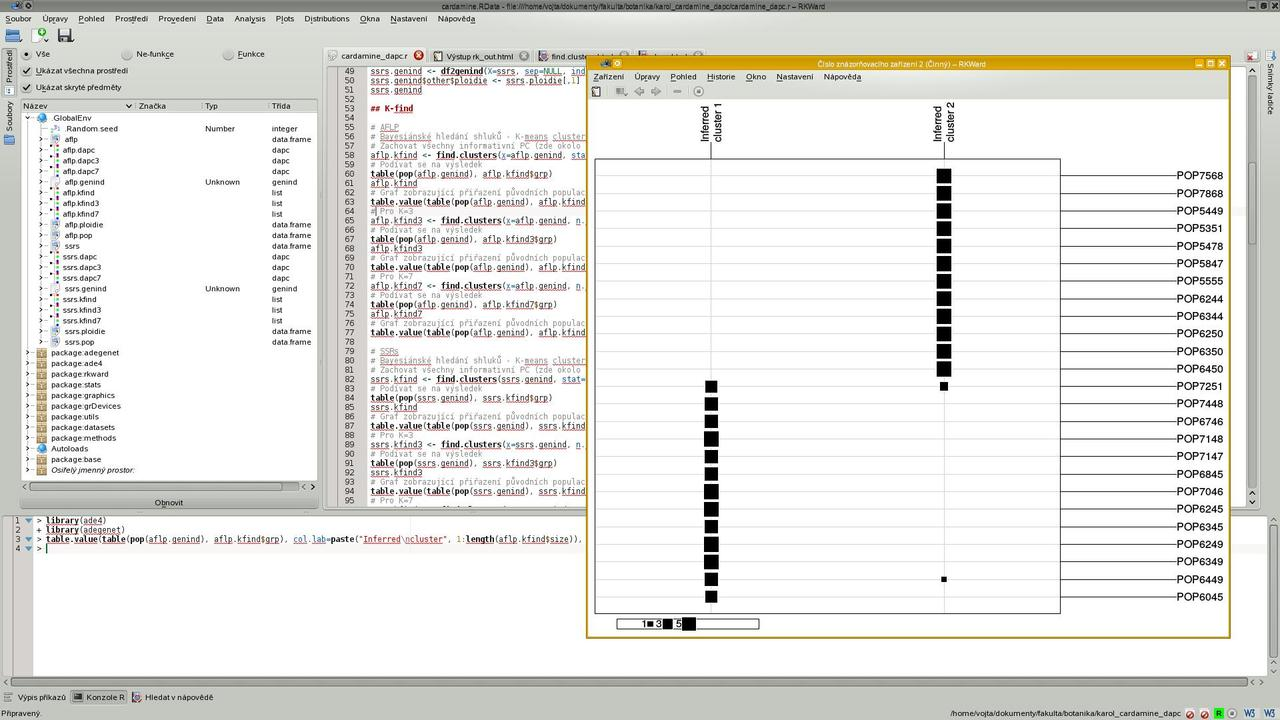
\includegraphics[width=\textwidth]{rkward.jpg}
\end{center}
\end{frame}

\begin{frame}{RStudio}
\begin{center}
  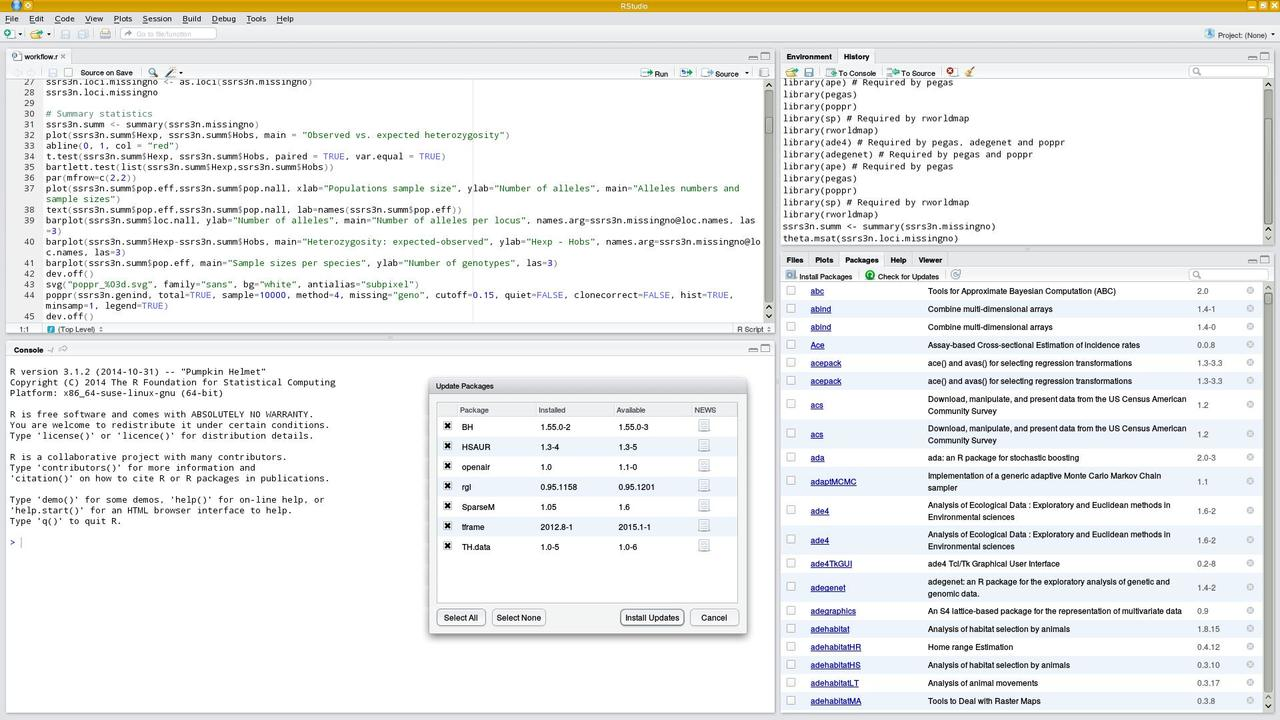
\includegraphics[width=\textwidth]{rstudio.jpg}
\end{center}
\end{frame}

\subsection{Installation}

\begin{frame}{MS Windows, Apple Mac OS X}
\begin{itemize}
 \item Got to \href{http://cran.at.r-project.org/}{http://cran.at.r-project.org/}
 \item Download appropriate version and install as usual
 \item Download and install selected GUI
 \item Most of packages are available as pre-compiled and can be immediately installed from R
 \item Convenient, but usually not tuned for particular computer architecture (type of CPU)
 \item Usually there are some problems every time new version of OS is released --- it takes time to modify and recompile packages for new version of OS
 \item You have to check for new version of R manually
\end{itemize}
\end{frame}

\begin{frame}{Linux --- general and Debian/Ubuntu}
\begin{itemize}
 \item R, and usually also GUI, is available in repositories --- use standard package management according to distribution
 \item Linux repositories provide automatic updates
 \item Packages are also partially available in repositories and can be installed and updated as usual application or from R
 \item Packages commonly have to be compiled -- R will do it automatically, just install basic Linux packages for building (in Debian and Ubuntu install package \textbf{build-essential})
 \item Debian (and derivatives): follow instructions at \href{http://cran.at.r-project.org/bin/linux/debian/}{http://cran.at.r-project.org/bin/linux/debian/}
 \item Ubuntu (and derivatives): follow instructions at \href{http://cran.at.r-project.org/bin/linux/ubuntu/}{http://cran.at.r-project.org/bin/linux/ubuntu/}
 \item As \textbf{<my.favorite.cran.mirror>} select \alert{cran.at.r-project.org}
\end{itemize}
\end{frame}

\begin{frame}{Linux --- openSUSE}
\begin{itemize}
 \item See instructions at \href{http://cran.r-project.org/bin/linux/suse/}{http://cran.r-project.org/bin/linux/suse/}
 \item Add repositories for your distribution
 \begin{itemize}
  \begin{footnotesize}
    \item \href{http://download.opensuse.org/repositories/devel:/languages:/R:/base/}{http://download.opensuse.org/repositories/devel:/languages:/R:/base/}
    \item \href{http://download.opensuse.org/repositories/devel:/languages:/R:/patched/}{http://download.opensuse.org/repositories/devel:/languages:/R:/patched/}
    \item \href{http://download.opensuse.org/repositories/devel:/languages:/R:/released/}{http://download.opensuse.org/repositories/devel:/languages:/R:/released/}
  \end{footnotesize}
 \end{itemize}
 \item Install packages \textbf{R-patched} (the R) and \textbf{rstudio} and/or \textbf{rkward}
 \item Install package \textbf{patterns-openSUSE-devel\_basis} for compilation of R packages when installing them from R (only some R packages are available in repositories)
 \item Compilation takes longer time and there are sometimes issues, but it can then provide higher performance\ldots
\end{itemize}
\end{frame}

\begin{frame}{Sources of R packages}
\begin{itemize}
 \item R CRAN \href{http://cran.r-project.org/}{http://cran.r-project.org/} --- main and largest source of R packages (over 6000 packages)
 \item Bioconductor \href{http://bioconductor.org/}{http://bioconductor.org/} --- mainly bioinformatic packages, genomic data ($\sim$1000 packages)
 \item R-Forge \href{http://r-forge.r-project.org/}{http://r-forge.r-project.org/} (over 1800 packages)
 \item RForge \href{http://www.rforge.net/}{http://www.rforge.net/} (much smaller)
 \item Omega Project for Statistical Computing \href{http://www.omegahat.org/}{http://www.omegahat.org/}
 \item And more\ldots
 \item Some packages are available from more resources --- same name for function can be used in different packages --- to distinguish them you can call functions like this: \textbf{muscle::read.fasta()} vs. \textbf{seqinr::read.fasta()} --- call function \textbf{read.fasta()} from package \textbf{muscle} \alert{or} \textbf{seqinr} (and their parameters can be different\ldots)
\end{itemize}
\end{frame}

\subsection{Let's start with R}

\begin{frame}{First steps in R}
\begin{multicols}{2}
  \begin{itemize}
    \item Linux: open any terminal, type \textbf{R} and hit Enter, Windows and Mac: find it as normal application in menu
    \item R is ruled by typing commands\ldots~:-)
    \item Use arrows up and down to navigate in history
    \item Ctrl+R works as reverse search --- searches typed string in history of commands
    \item We will mostly use GUI
  \end{itemize}
  \columnbreak
  \begin{flushright}
    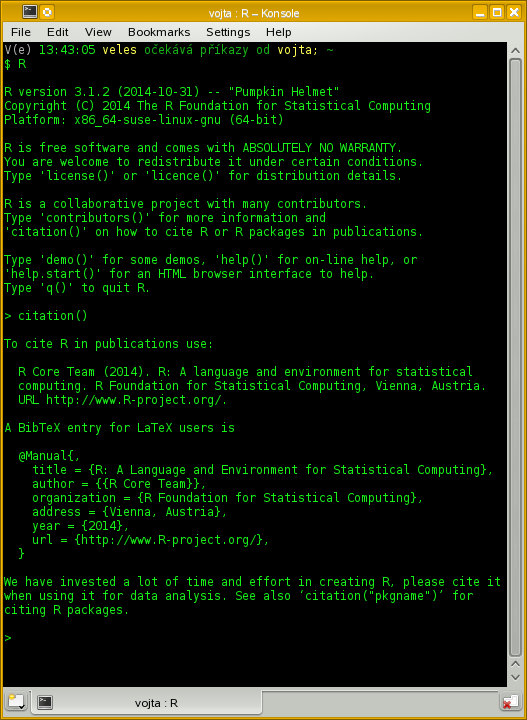
\includegraphics[width=5cm]{rkonsole.png}
  \end{flushright}
\end{multicols}
\end{frame}

\begin{frame}{How it works}
\begin{itemize}
 \item General look of R commands:
 \item \splus/function(argument1="SomeName", argument2=SomeVariable, argument3=8)/
 \item \splus/ModifiedObject <- SomeFunction(argument1=MyData, argument2=TRUE)/
 \item Object is on the left: ``<-'' says to insert result of the function on the right into the object
 \item Functions have various parameters/arguments (in brackets, separated by comas): argument=ItsValue
 \item Arguments are named --- if you keep order, no need to name them:
 \item \splus/SomeFunction(MyData, TRUE, 123, "SomeName")/
 \item When only some of the arguments are in use, use the names (order doesn't matter any more)
 \item \splus/SomeFunction(argument2=TRUE, argument3=123, argument1=MyData)/
\end{itemize}
\end{frame}

\begin{frame}[fragile]{Get help in R}
  \begin{spluscode}
    # "#" marks comments - notes within code which are not executed
    help(function) # Help for particular function (package must be loaded)
    ?function # Help for particular function (package must be loaded)
    ??SearchedTerm # Search for the term within all installed packages
    help.search("searched phrase") # Search for the phrase within all
      # installed packages - return list of hits sorted according to
      # type and package (i.e. package::function)
    install.package("sos") # More comprehensive search from package sos
    library(sos)
    findFN("function")# Search for function name
  \end{spluscode}
\alert{\textbf{?}} shows help for questioned function:
\begin{multicols}{2}
  \begin{itemize}
    \item Name of the package (top left)
    \item Function name (headline)
    \item Description
    \item Usage
    \item Comments on arguments
    \item Details
    \item About author(s)
    \item References to cite
    \item Example code
  \end{itemize}
\end{multicols}
\end{frame}

\begin{frame}[fragile]{Where we are?}
\begin{itemize}
 \item In Linux, R starts in current directory (use \textbf{cd} to change it before launching R)
 \item Set and check working directory in R:
\end{itemize}
  \begin{spluscode}
    setwd("/some/path/") # Or "~/...". In Windows "C:\..."
    getwd() # Verifies where we are
    dir() # Lists files and folders on the disk
    ls() # Lists currently available R objects
  \end{spluscode}
\begin{itemize}
 \item In Windows (File | working directory) or in RStudio (Session | Set working directory) set it in menu or by above command
 \item R saves history of commands into \textbf{.Rhistory} file within working directory (by default hidden in Linux/Mac)
 \item When closing R by \textbf{q()} you can save all R data in \textbf{.RData} file and it can be loaded next time
 \item RStudio and RKWard help with this very much
\end{itemize}
\end{frame}

\begin{frame}{Materials to help you\ldots}
\begin{itemize}
 \item Follow all code we will use at \href{https://trapa.cz/sites/default/rcourse/course_commands.html}{https://trapa.cz/sites/default/rcourse/course\_commands.html}
 \item Download the script from \href{https://trapa.cz/sites/default/rcourse/course_commands.r}{https://trapa.cz/sites/default/rcourse/course\_commands.r}, use it and write your comments and notes to it during the course
 \item \alert{Note:} Open the R script in some \alert{good} \href{http://texteditors.org/cgi-bin/wiki.pl?PickingATextEditor}{text editor} --- showing syntax highlight, line numbers, etc. (\alert{NO} Windows notepad); the file is in UTF-8 encoding and with Linux end of lines (so that too silly programs like Windows notepad won't be able to open it correctly)
 \item Information about the course: \href{https://trapa.cz/en/course-molecular-data-r-2015}{https://trapa.cz/en/course-molecular-data-r-2015} or \href{https://trapa.cz/cs/kurz-molekularni-data-r}{https://trapa.cz/cs/kurz-molekularni-data-r}
\end{itemize}
\end{frame}

\subsection{Basic operations in R}

\begin{frame}{Types of objects}
\begin{itemize}
 \item Vectors --- numbers or characters
 \item Matrices --- columns are of same type (numeric, character, etc.) and the same length
 \item Arrays --- like matrices, but with possibly more dimensions
 \item Data frames --- more general --- columns can be of different type
 \item Lists --- ordered collections of objects (vectors, matrices, \ldots) --- not necessarily of the same type
 \item Factors --- a vector of levels, e.g. populations, colours, etc.
 \item More ``advanced'' objects to store plots, genetic data, \ldots
 \begin{itemize}
  \item Commonly called ``S3'' and ``S4'' objects
  \item Technically commonly just lists putting together various information
  \item We will meat many of them\ldots
 \end{itemize}
 \item Functions require particular object types --- take care about it
\end{itemize}
\end{frame}

\begin{frame}{Popular object classes (we are going to use) I}
\begin{itemize}
 \item dist --- distance matrices
 \item genind --- stores various genetic information for individuals
 \item genpop --- like genind, but on population level
 \item genlight --- variant of genind to store large multiple genomes
 \item SNPbin --- stores large SNP data for single genome
 \item DNAbin --- stores DNA sequences (aligned or not)
 \item haplotype --- unique sequences from DNAbin
 \item alignment --- aligned sequences (seqinr)
 \item phyDat --- ``preparation'' of data for some phylogenetic analysis
 \item loci -- extension of DF, stores information about loci
 \item hclust -- output of hierarchical clustering, can be converted to phylo
 \item treeshape --- derived from hclust
\end{itemize}
\end{frame}

\begin{frame}[fragile]{Popular object classes (we are going to use) II}
\begin{itemize}
 \item phylo --- phylogenetic information, typically trees
 \item phylo4 --- derived from phylo, S4 instead of S3
 \item matching -- binary phylogenetic trees
 \item haplonet --- networks without reticulation
 \item spca --- results of sPCA
 \item pco; dudi --- results of PCA, PCoA, \ldots
 \item dapc --- results of DAPC
 \item and more\ldots common task is converting among formats\ldots
 \item \ldots not all formats are (easily) convertable amon each other\ldots
\end{itemize}
To get information about content of each data type see
\splus/getClassDef("genind") # Or any other class name/
There are information about slots within that classes you can access.
\end{frame}

\begin{frame}{Conversions among data types I}
  \begin{tabular}{llll}
    \textbf{From} & \textbf{To} & \textbf{Command} & \textbf{Package}\\
    phylo & phylo4 & as(x, "phylo4") & phylobase\\
    phylo & matching & as.matching(x) & ape\\
    phylo & treeshape & as.treeshape(x) & apTreeshape\\
    phylo & hclust & as.hclust(x) & ape\\
    phylo & prop.part & prop.part(x) & ape\\
    phylo & splits & as.splits(x) & phangorn\\
    phylo & evonet & evonet(x, from, to) & ape\\
    phylo & network & as.network(x) & ape\\
    phylo & igraph & as.igraph(x) & ape\\
    phylo4 & phylo & as(x, "phylo") & phylobase\\
    matching & phylo & as.phylo(x) & ape\\
    treeshape & phylo & as.phylo(x) & apTreeshape\\
    splits & phylo & as.phylo(x) & phangorn
  \end{tabular}
\end{frame}

\begin{frame}{Conversions among data types II}
  \begin{tabular}{llll}
    \textbf{From} & \textbf{To} & \textbf{Command} & \textbf{Package}\\
    splits & networx & as.networx(x) & phangorn\\
    evonet & phylo & as.phylo(x) & ape\\
    evonet & networx & as.networx(x) & ape\\
    evonet & network & as.network(x) & ape\\
    evonet & igraph & as.igraph(x) & ape\\
    haploNet & network & as.network(x) & pegas\\
    haploNet & igraph & as.igraph(x) & pegas\\
    hclust & phylo & as.phylo(x) & ape\\
    hclust & dendrogram & as.dendrogram(x) & stats\\
    DNAbin & character & as.character(x) & ape\\
    DNAbin & alignment & as.alignment(x) & ape\\
    DNAbin & phyDat & as.phyDat(x) & phangorn\\
    DNAbin & genind & DNAbin2genind(x) & adegenet\\
    character & DNAbin & as.DNAbin(x) & ape
  \end{tabular}
\end{frame}

\begin{frame}{Conversions among data types III}
  \begin{tabular}{llll}
    \textbf{From} & \textbf{To} & \textbf{Command} & \textbf{Package}\\
    character & loci & as.loci(x) & pegas\\
    alignment & DNAbin & as.DNAbin(x) & ape\\
    alignment & phyDat & as.phyDat(x) & phangorn\\
    alignment & character & as.matrix(x) & seqinr\\
    alignment & genind & alignment2genind(x) & adegenet\\
    phyDat & DNAbin & as.DNAbin(x) & phangorn\\
    phyDat & character & as.character(x) & phangorn\\
    loci & genind & loci2genind(x) & pegas\\
    loci & data frame & class(x) <- "data.frame" & \\
    genind & loci & genind2loci(x) & pegas\\
    data frame & phyDat & as.phyDat(x) & phangorn\\
    data frame & loci & as.loci(x) & pegas\\
    data frame & genind & df2genind(x) & adegenet\\
    matrix & phyDat & as.phyDat(x) & phangorn
  \end{tabular}
\end{frame}

\begin{frame}[fragile]{Basic operations with data I}
  \begin{spluscode}
    x <- c(1, 2, 3, 4, 5) # Creates vector (see also ?rep)
    c() # Is generic function to concatenate objects into new one
    length(x) # Length of the object - for matrices and DF use dim()
    str(x) # Information about structure of the object, try also ls.str()
    mode(x) # Gets type of storage mode of the object
    class(x) # Shows class of the object
    x[2] # Shows second element of the object
    x <- x[-5] # Removes fifth element
    y <- matrix(data=5:20, nrow=4, ncol=4) # Creates a matrix
    is.matrix(y) # Is it matrix? Try is.<TAB><TAB>
    # TAB key shows available functions and objects starting by typed text
    y # Prints the matrix
    y[,2] # Prints second column
    y[3,] # Prints third row
    y[4,3] # Prints element from fourth row and third column
    x <- y[2,] # Replaces "x" by second row of "y" (no warning)
    # R doesn't ask neither notifies when overwriting objects! Be careful!
  \end{spluscode}
\end{frame}

\begin{frame}[fragile]{Basic operations with data II}
  \begin{spluscode}
    rm(x) # Deletes x
    y[,1:3] # Prints first through third column of the matrix
    y[3,] <- rep(x=20, each=4) # Replaces third line by value of 20
    y[y==20] <- 10 # If value of y's element is 20, replace it by 10
    summary(y) # Basic statistics - according to columns
    colnames(y) <- c("A", "B", "C", "D") # Set column names
    # Objects and functions are without quotation marks; files, text with
    colnames(y) # Prints column names, use rownames() in same way
    y[,"C"] # Prints column C (R is case sensitive!)
    t(y) # Transposes the matrix
    y <- as.data.frame(y) # Turns into DF (see other functions as.*)
    y[y==17] <- "NA" # Removes values of 17
    y$B # Gets variable B of data frame y ($ works similarly in S3 objects)
    save(list=ls(), file="test.RData") # Saves all objects during the work
    load("test.RData") # Loads saved R environment with all objects
    # When loading saved project, you have to load again libraries and
    # scripts (see further), data objects are restored
  \end{spluscode}
\end{frame}

\subsection{Packages for our work}

\begin{frame}[fragile, label=repos]{Set repositories}
  \begin{spluscode}
    # Basic package installation
    install.packages("PackageName") # Case sensitive!
    ?install.packages # Shows all available parameters
    # We will need extra repositories:
    options(repos=c("http://cran.at.r-project.org",
      "http://r-forge.r-project.org/", "http://www.rforge.net/",
      "http://bioconductor.statistik.tu-dortmund.de/packages/3.1/bioc",
      "http://bioconductor.statistik.tu-dortmund.de/packages/3.1/data/
      annotation", "http://bioconductor.statistik.tu-dortmund.de/
      packages/3.1/data/experiment",
      "http://bioconductor.statistik.tu-dortmund.de/packages/3.1/extra"))
    getOption("repos") # Shows actual repositories
    options() # Generic function to modify various settings
    ?options # Gives details
  \end{spluscode}
\begin{itemize}
 \item \alert{All the time keep newest version of R and and newest versions of packages!}
 \item Installation of multiple packages may sometimes fail --- install then packages in smaller groups or one by one
\end{itemize}
\end{frame}

\begin{frame}[fragile]{Install needed packages}
  \begin{spluscode}
    install.packages(pkgs=c("Geneland", "PBSmapping", "ParallelStructure",
      "RandomFields", "RgoogleMaps", "TeachingDemos", "XML", "ade4",
      "adegenet", "adephylo", "akima", "ape", "colorspace", "combinat",
      "corrplot", "fields", "gplots", "grid", "ips", "lattice", "mapdata",
      "mapproj", "maps", "maptools", "muscle", "pegas", "permute",
      "phangorn", "phyloch", "phytools", "polysat", "poppr", "rworldmap",
      "seqinr", "sp", "spam", "tcltk", "vegan"), repos=getOption("repos"),
      dependencies=TRUE)
    library(package) # Loads installed package (we will do it on the fly)
    update.packages(repos=getOption("repos")) # Updates installed packages
  \end{spluscode}
\begin{block}{Installation of packages in GUI}
  \begin{footnotesize}
    \begin{itemize}
      \item RStudio: set repositories by command from slide~\ref{repos} and in bottom right pane select ``Packages'' and click on ``Install Packages''\ldots
      \item RKWard: go to menu ``Settings'' | ``Configure 'RKWard''' and select ``Packages R''. Add URLs pf repositories from slide~\ref{repos}. OK. Go to menu ``Settings'' | ``Manage R packages'', click to ``Install\ldots'', select and install desired packages\ldots
    \end{itemize}
  \end{footnotesize}
\end{block}
\end{frame}

\begin{frame}[fragile]{Bioconductor}
\begin{itemize}
 \item Tools for analysis of genomic data, see \href{http://bioconductor.org/}{http://bioconductor.org/}
 \item To install it, add appropriate repositories (repository use to have same version number as R --- change them accordingly when upgrading R) or use Bioconductor's special function (recommended by Bioconductor):
\end{itemize}
  \begin{spluscode}
    # Load basic Bioconductor function
    source("http://bioconductor.org/biocLite.R")
    # Get help how to use it
    ?biocLite
    # Install packages
    biocLite(c("package1", "package2", "..."))
    # Upgrades installed Bioconductor packages
    biocLite("BiocUpgrade")
  \end{spluscode}
\begin{itemize}
 \item Explore available packages: \href{http://bioconductor.org/packages/release/BiocViews.html}{http://bioconductor.org/packages/release/BiocViews.html}
\end{itemize}
\end{frame}

\section{Data}

\begin{frame}[fragile]{Population genetics and phylogenetics in R}{Microsatellites, AFLP, SNP \& sequences}
\begin{multicols}{2}
  \begin{itemize}
    \item Now we will use mainly packages \href{http://adegenet.r-forge.r-project.org/}{adegenet} and \href{http://grunwaldlab.cgrb.oregonstate.edu/poppr-r-package-population-genetics}{poppr}
    \item Other important genetic packages: \href{http://ape-package.ird.fr/}{ape}, \href{http://pbil.univ-lyon1.fr/ADE-4/}{ade4} and \href{http://ape-package.ird.fr/pegas.html}{pegas}
    \item Dominant/co-dominant marker data of any ploidy level including SSRs, SNP, and AFLP
    \item Most of methods are able for polyploids (although not all)
    \item Some methods are unavailable for dominant (presence/absence) data
    \item Mixing of ploidy levels is tricky --- it doesn't matter when data are encoded as PA, otherwise it is problematic
  \end{itemize}
  \begin{spluscode}
    library(ape)
    library(ade4)
    library(adegenet)
    library(pegas)
    library(poppr)
  \end{spluscode}
\end{multicols}
\end{frame}

\subsection{Microsatellites}

\begin{frame}[fragile]{Load data}
Source data:
\begin{verbatim}
    pop msta93 msta101 msta102 msta103 msta105 msta131...
H01 He 269/269 198/198 221/223 419/419 197/197 196/196...
H02 He 275/283 198/198 221/223 419/419 193/193 168/190...
... ......     ...     ...     ...     ...     ...    ...
\end{verbatim}
  \begin{spluscode}
    # Load training data (Taraxacum haussknechtii from Macedonia)
    hauss.loci <- read.loci(file="http://trapa.cz/sites/default/rcourse/
      haussknechtii_ssrs.txt", header=TRUE, loci.sep="\t", allele.sep="/",
      col.pop=2, col.loci=3:14, row.names=1) # \t means TAB key
    # Data control
    hauss.loci
    print(hauss.loci, details=TRUE)
  \end{spluscode}
\begin{footnotesize}
  First line starts with empty cell (if \textbf{header} is presented), there can be any extra column, just take care about \textbf{col.loci}. \textbf{row.names} are individual names (firs column). Take care about \textbf{loci.sep} (here TAB) and \textbf{allele.sep} according to data formatting.
\end{footnotesize}
\end{frame}

\begin{frame}[fragile]{Prepare genind object for analysis and load coordinates}
  \begin{spluscode}
    # Conversion of loci to genind - used for many analysis
    hauss.genind <- loci2genind(hauss.loci)
    # See population names
    pop(hauss.genind)
    hauss.genind$pop.names # "$" separates extra slots within object
  \end{spluscode}
Coordinates can be in any projection or scale --- according to aim\\
Source data:
\begin{verbatim}
Ind  lon      lat
H01  21.3333  41.1
...  ...      ...
\end{verbatim}
  \begin{spluscode}
    # Read coordinates
    hauss.coord <- read.csv("http://trapa.cz/sites/default/rcourse/
      haussknechtii_coordinates.csv", header=TRUE, sep="\t", quote="",
      dec=".", row.names=1)
    hauss.coord
  \end{spluscode}
\begin{footnotesize}
  Take care about parameters of \textbf{read.csv()}! See \textbf{?read.csv} for details.
\end{footnotesize}
\end{frame}

\begin{frame}[fragile]{Add coordinates to genind and create genpop object}
  \begin{spluscode}
    # Add coordinates - note identification of slots within object
    hauss.genind$other$xy <- hauss.coord
    # See result
    hauss.genind$other$xy
    hauss.genind
    # Removes missing data - see ?missingno for types of dealing them
    hauss.genind <- missingno(pop=hauss.genind, type="mean", cutoff=0.1)
    # Convert corrected genind to loci
    hauss.loci.cor <- genind2loci(hauss.genind)
    # Writes loci file to the disk
    write.loci(hauss.loci.cor, file="hauss.loci.cor.txt",
      loci.sep="\t", allele.sep="/")
    # Conversion to genpop - for population-level analysis
    hauss.genpop <- genind2genpop(hauss.genind, missing="NA",
      process.other=TRUE)
    # See result
    hauss.genpop
  \end{spluscode}
\end{frame}

\begin{frame}[fragile]{Import existing data set from popular software}
  \begin{spluscode}
    read.genalex() # poppr - reads *.csv file
    read.fstat() # adegenet - reads *.dat files, only haploid/diploid data
    read.genetix() # adegenet - reads *.gtx files, only haploid/diploid data
    read.genepop() # adegenet - reads *.gen files, only haploid/diploid data
    read.structure() # adegenet - reads *.str files, only haploids/diploids
    import2genind() # adegenet - more automated version of above functions
  \end{spluscode}
\begin{block}{One function rules them all\ldots}
  All those functions (including read-loci and read.csv) are only modifications of \textbf{read.table()}. You can use it directly to import any data. Look at \textbf{?read.table} and play with it. Take care about parameters. Does the table use quotes to mark cell (quote=\ldots)? How are columns separated (sep=\ldots)? Is there a header with names of populations/loci/whatever (header=T/F)? What is decimal separator (dec=\ldots)? Are there row names (used typically as names of individuals; row.names=\ldots)? Check data after import!
\end{block}
\end{frame}

\begin{frame}[fragile]{Import of polyploid microsatellites}
\begin{itemize}
 \item adegent, poppr and related packages can for most of functions handle any ploidy level (but no mixing of various ploidy levels for microsatellites)
 \item polysat can handle mixed ploidy levels for microsatellites, but range of methods is limited
\end{itemize}
As for AFLP, we need two files: the data matrix and individual's populations:
\begin{verbatim}
       msat58      msat31      msat78      msat61      ...
ala1   124/124/124 237/237/237 164/164/172 136/136/138 ...
ala2   124/124/124 237/237/237 164/164/172 136/136/138 ...
ala4-1 124/124/124 237/237/237 164/164/172 136/136/138 ...
...    ...         ...         ...         ...         ...
\end{verbatim}
\end{frame}

\begin{frame}[fragile]{How to import polyploid microsatellites}
  \begin{spluscode}
    # Import if table is as usual. Last column contains populations
    tarax3n.table <- read.table("http://trapa.cz/sites/default/rcourse/
      tarax3n.txt", header=TRUE, sep="\t", quote="", row.names=1)
    # Check the data
    tarax3n.table
    class(tarax3n.table)
    dim(tarax3n.table)
    # See parameter "X" - we don't import whole tarax3n.table as last column
    # contains populations - this column we use for "pop" parameter (note
    # different style of calling the column - just to show the possibility).
    # Check "ploidy" and "ncode" (how many digits code one allele - must be
    # same everywhere). See ?df2genind for more details.
    tarax3n.genind <- df2genind(X=tarax3n.table[,1:6], sep="/", ncode=3,
      pop=tarax3n.table[["pop"]], missing=NA, ploidy=3, type="codom")
    # See resulting genind object
    tarax3n.genind
    summary(tarax3n.genind)
  \end{spluscode}
\end{frame}

\subsection{AFLP}

\begin{frame}[fragile]{Import of AFLP data --- background}
Source data (two files - AFLP data with individual names and populations)
\begin{multicols}{2}
AFLP -- presence/absence data:
\begin{verbatim}
     L1 L2 L3 L4 L5 L6 L7 L8 L9 ...
Ind1 0  0  1  1  1  0  0  0  1  ...
IndG 0  0  1  1  0  0  0  0  0  ...
...  ...  ...
\end{verbatim}
Individual's populations:
\begin{verbatim}
POP
pop1
popZ
...
\end{verbatim}
\columnbreak
\begin{itemize}
 \item Use any names, just keep one word (no spaces) and don't use special characters
 \item Keep names of loci as simple as possible, there are some issues when they contain dots
 \item As soon as one line of data = one individual, ploidies and their mixing doesn't matter
 \item Not all methods are available/meaningful for PA
\end{itemize}
\end{multicols}
\end{frame}

\begin{frame}[fragile]{Import of AFLP data --- the code}
  \begin{spluscode}
    amara.aflp <- read.table(file="http://trapa.cz/sites/default/rcourse/
      amara_aflp.txt", header=TRUE, sep="\t", quote="")
    amara.aflp
    dim(amara.aflp)
    class(amara.aflp) # Must be matrix or data frame
    # Populations - just one column with population names for all inds
    amara.pop <- read.table(file="http://trapa.cz/sites/default/rcourse/
      amara_pop.txt", header=TRUE, sep="\t", quote="")
    amara.pop
    # You can use just one file, where populations are in last column and
    # in df2genind() use for example X=aflp[,1:XXX] and pop=aflp[,YYY]
    # Create genind object - ind.names and loc.names are taken from X
    aflp.genind <- df2genind(X=amara.aflp, sep=NULL, ind.names=NULL,
      loc.names=NULL, pop=amara.pop[,1], missing=NA, type="PA")
    aflp.genind
    summary(amara.aflp)
    # You can add any other variables into genind$other$XXX
  \end{spluscode}
\end{frame}

\subsection{Notes about data}

\begin{frame}[fragile]{Another data manipulation}
SNPs can be into genind imported in same way as AFLP
  \begin{spluscode}
    genind2df() # adegenet - export into data frame
    genind2genalex() # poppr - export for genalex
    splitcombine() # poppr - edits population hierarchy
    popsub() # poppr - extracts only selected population(s)
    clonecorrect() # poppr - corrects for clones
    informloci() # poppr - removes uninformative loci
    seppop() # adegenet - separates populations from genind or genlight
    seploc() # adegenet - splits genind, genpop or genlight by markers
    # seppop and seploc return lists of objects - for further analysis
    # read manual pages (?...) of those functions before usage
  \end{spluscode}
\end{frame}

\begin{frame}{Notes about getting data into R}
\begin{itemize}
 \item When importing fragmentation data, we somehow use function \textbf{read.table()} --- it is important to understand it
 \item I recommend to use TAB (TSV --- tab separated values; encoded as ``\textbackslash t'' in R) to separate columns (no quotation marks, no commas)
 \item When importing microsatellites, all alleles \textbf{must} have same number of digits. Separate alleles by ``/'', ``|'' or something similar and correctly specify it in \textbf{read.loci()} or \textbf{df2genind()}
 \item Do not use underscores (``\_'') to name objects in R --- only numbers, letters, dots and minuses
 \item \textbf{read.loci()} sometimes doesn't work correctly on AFLP or polyploid microsatellites --- try \textbf{write.table()} instead\ldots
 \item Theoretically, genind object could be currently able to store mixing ploidy data, but most of analysis will probably fail\ldots
\end{itemize}
\end{frame}

\subsection{DNA sequences, SNP}

\begin{frame}[fragile]{Import of DNA data}
  \begin{spluscode}
    # Reading FASTA (reads also another formats, see ?read.dna)
    # Sequences of flu viruses from various years
    usflu.dna <- read.dna(file="http://adegenet.r-forge.r-project.org/
      files/usflu.fasta", format="fasta")
    # Another possibility (only for FASTA alignments, same result):
    usflu.dna <- fasta2DNAbin(file="http://adegenet.r-forge.r-project.org/
      files/usflu.fasta") # Normally keeps only SNP -- see ?fasta2DNAbin
    # Check the object
    usflu.dna
    class(usflu.dna)
    as.character(usflu.dna)[1:5,1:10]
    # Read anotations
    usflu.annot <- read.csv("http://adegenet.r-forge.r-project.org/files/
      usflu.annot.csv", header=TRUE, row.names=1)
    head(usflu.annot) # See result
    # Convert DNAbin to genind - only polymorphic loci (SNPs) are retained
    # When converting DNAbin to genind, the sequences must be aligned!
    usflu.genind <- DNAbin2genind(x=usflu.dna, pop=usflu.annot[["year"]])
  \end{spluscode}
\end{frame}

\begin{frame}[fragile]{Import sequences from GeneBank}
  \begin{spluscode}
    # read.fasta() from seqinr package reads DNA or AA in FASTA format
    # returns a list (DNAbin is for us now better choice)
    usflu.dna <- read.fasta(file="http://adegenet.r-forge.r-project.org/
      files/usflu.fasta", seqtype="DNA"
    # Importingsequences according to sequence ID
    # data from http://www.ncbi.nlm.nih.gov/popset/608602125 (Meles meles)
    meles.dna <- read.GenBank(c("KJ161355.1", "KJ161354.1", "KJ161353.1",
      "KJ161352.1", "KJ161351.1", "KJ161350.1", "KJ161349.1", "KJ161348.1",
      "KJ161347.1", "KJ161346.1", "KJ161345.1", "KJ161344.1", "KJ161343.1",
      "KJ161342.1", "KJ161341.1", "KJ161340.1", "KJ161339.1", "KJ161338.1",
      "KJ161337.1", "KJ161336.1", "KJ161335.1", "KJ161334.1", "KJ161333.1",
      "KJ161332.1", "KJ161331.1", "KJ161330.1", "KJ161329.1", "KJ161328.1"))
    meles.dna
    class(meles.dna)
    # Converts DNAbin to genind - extracts SNP - for large datasets can be
    # computationally very intensive
    meles.genind <- DNAbin2genind(meles.dna)
  \end{spluscode}
To query on-line database as through web interface we use \href{http://cran.r-project.org/web/packages/seqinr/index.html}{seqinr}.
\end{frame}

\begin{frame}[fragile]{Query on-line sequence databases}
  \begin{spluscode}
    library(seqinr)
    choosebank() # Genetic banks available for seqinr
    choosebank("embl") # Choose some bank
    ?query # See how to construct the query
    # Query selected database - there are much possibilities
    nothofagus <- query(listname="nothofagus",
      query="SP=Nothofagus AND K=rbcl", verbose=TRUE)
    # See the sequences information
    nothofagus$req
    # Get the sequences as a list
    nothofagus.sequences <- getSequence(nothofagus$req)
    # See sequences
    nothofagus.sequences
    # Get annotations
    nothofagus.annot <- getAnnot(nothofagus[["req"]])
    # Close the bank when work is over
    closebank()
    # Convert sequences from a list to DNAbin (functions as.DNAbin*)
    nothofagus.dna <- as.DNAbin.list(nothofagus.sequences)
  \end{spluscode}
\end{frame}

\begin{frame}[fragile]{Checking SNPs}
\begin{multicols}{2}
  \begin{spluscode}
    # Position of polymorphism within
    # alignment - snpposi.plot requires
    # input data in form of matrix
    snpposi.plot(x=as.matrix(
      meles.dna), codon=FALSE)
    # Position of polymorphism within
    # alignment - differentiating codons
    snpposi.plot(as.matrix(meles.dna))
    # When converting to genind object,
    # only polymorphic loci are kept - 
    # threshold for polymorphism can
    # be arbitrary
    meles.genind <- DNAbin2genind(x=
      meles.dna, polyThres=0.01)
    # Test of random distribution of SNP
    snpposi.test(as.matrix(meles.dna))
  \end{spluscode}
  \begin{flushright}
    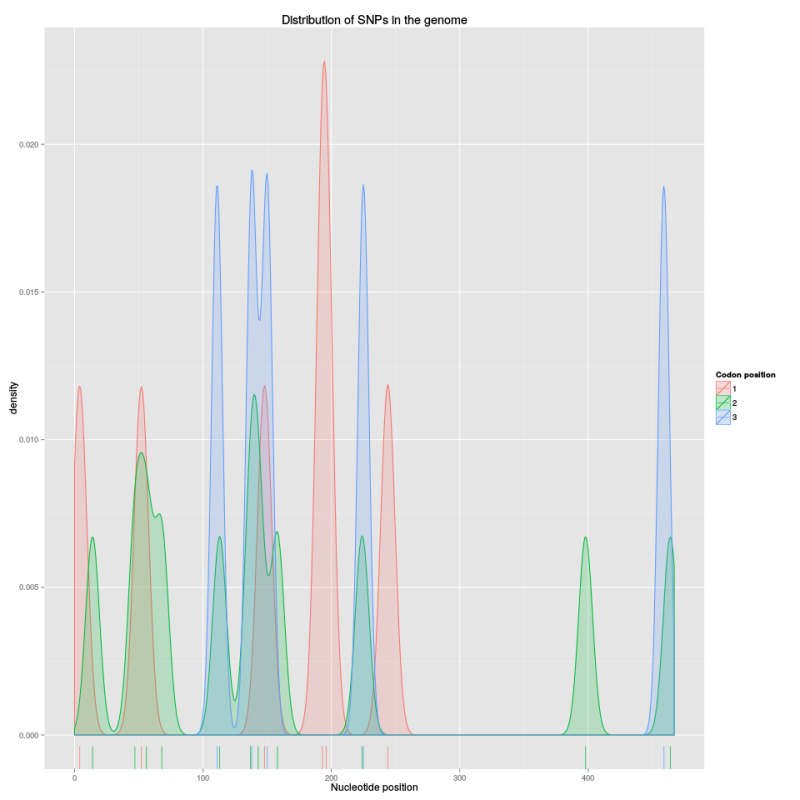
\includegraphics[height=6cm]{snpposi.png}
  \end{flushright}
\end{multicols}
\end{frame}

\begin{frame}[fragile]{Importing SNP}
Import from \href{http://pngu.mgh.harvard.edu/~purcell/plink/}{PLINK} requires saving of data with option \href{http://pngu.mgh.harvard.edu/~purcell/plink/dataman.shtml#recode}{``-recodeA''}:
\splus/read.PLINK(file="PLINKfile", ...) # See ?readPLINK/
Extracting SNP from alignments reads FASTA alignments and keep only SNPs. The method is relatively efficient even for large data sets with several genomes:
  \begin{spluscode}
    usflu.genlight <- fasta2genlight(file=
      "http://adegenet.r-forge.r-project.org/files/usflu.fasta",
      quiet=FALSE, saveNbAlleles=TRUE)
    ?fasta2genlight # Function has several options to speed up reading
    # If it crashes (on Windows), try add parameter "parallel=FALSE"
  \end{spluscode}
\begin{itemize}
 \item For small datasets it doesn't matter if resulting dataset is genind or genlight, for large genlight is more efficient
\end{itemize}
  \begin{spluscode}
    # Convert genlight to genind
    usflu.genind <- as.genind(usflu.genlight)
    # Resulting data matrix might be slightly different than when using
    # DNAbin2genind - depends on used settings
  \end{spluscode}
\end{frame}

\begin{frame}{Notes about using genlight (vs. genind)}
\begin{itemize}
 \item Genlight is ``just'' version of more common genind object to store large data sets with (nearly) complete multiple genomes
 \item ``Large'' is tricky --- there is no easy criterion --- try genind and when work fails because of not enough computer resources, go on with genlight
 \item Can be quickly converted to genind (not back)
 \item Use is basically same as when working with genind --- but not all functions are able to deal with it (on the other hand, others are optimised to work well on large data sets)
 \item SNPbin is version of genind/genlight to store one large genome --- serves basically as storage, no need to deal with it
 \item genlight allows varying ploidy level --- genind has issues with it
\end{itemize}
\end{frame}

\subsection{Export}

\begin{frame}[fragile]{Export data}
  \begin{spluscode}
    # Convert genind into DF using genind2genotype() or genind2df()
    hauss.df <- genind2genotype(x=hauss.genind, pop=hauss.genind@pop,
      res.type="matrix")
    hauss.df <- genind2df(x=hauss.genind, pop=NULL, sep="/",
      usepop=TRUE, oneColPerAll=FALSE)
    write.table(x=hauss.df, file="haussdata.txt", quote=FALSE,
      sep="\t", na="NA", dec=".", row.names=TRUE, col.names=TRUE)
    # Export of DNA sequences into FASTA format
    write.dna(x=usflu.dna, file="usflu.fasta", format="fasta",
      append=FALSE, nbcol=6)
    write.fasta(sequences=meles.dna, names=names(meles.dna),
      file.out="meles.fasta", open="w")
    # Export trees (objects of class phylo)
    # Writes tree(s) in NEWICK format
    write.tree(phy=hauss.nj.bruvo, file="haussknechtii.nwk")
    # Writes tree(s) in NEXUS format
    write.nexus(hauss.nj.bruvo, file="haussknechtii.nexus")
  \end{spluscode}
\end{frame}

\section{Basic analysis}

\subsection{First look at the data}

\begin{frame}[fragile]{Descriptive statistics I}
We will now work mainly with diploid SSRs for \textit{Taraxacum haussknechtii}, you can try other data examples by yourselves
  \begin{spluscode}
    # Get summary - names and sizes of populations,
    # heterozygosity, some info about loci
    hauss.summ <- summary(hauss.genind)
    # Plot expected vs. observed heterozygosity
    # it looks like big difference
    plot(x=hauss.summ$Hexp, y=hauss.summ$Hobs,
      main="Observed vs expected heterozygosity",
      xlab="Expected heterozygosity", ylab="Observed heterozygosity")
    abline(0, 1, col="red")
    # T-test of difference between
    # observed and expected heterozygosity - strongly significant
    t.test(x=hauss.summ$Hexp, y=hauss.summ$Hobs, paired=TRUE, var.equal=T)
    # Bartlett's K-squared of difference
    # between observed and expected heterozygosity - not significant
    bartlett.test(list(hauss.summ$Hexp,hauss.summ$Hobs))
  \end{spluscode}
\end{frame}

\begin{frame}[fragile]{Descriptive statistics II}
  \begin{spluscode}
    # Create pane with some information
    par(mfrow=c(2,2)) # Divide graphical devices into 4 smaller spaces
    # Plot alleles number vs. population sizes
    plot(x=hauss.summ$pop.eff, y=hauss.summ$pop.nall, xlab="Populations
      sample size", ylab="Number of alleles", main="Alleles numbers and
      sample sizes", col="red", pch=20)
    # Add text description to the point
    text(x=hauss.summ$pop.eff, y=hauss.summ$pop.nall,
      lab=names(hauss.summ$pop.eff), cex=1.5)
    # Barplots of various data
    barplot(height=hauss.summ$loc.nall, ylab="Number of alleles",
      main="Number of alleles per locus",
      names.arg=hauss.genind@loc.names, las=3)
    barplot(height=hauss.summ$Hexp-hauss.summ$Hobs, main="Heterozygosity:
      expected-observed", ylab="Hexp - Hobs",
      names.arg=hauss.genind@loc.names, las=3)
    barplot(height=hauss.summ[["pop.eff"]], main="Sample sizes per
      population", ylab="Number of genotypes", las=3)
  \end{spluscode}
\end{frame}

\subsection{Statistics}

\begin{frame}[fragile]{Graphs from previous two slides}
  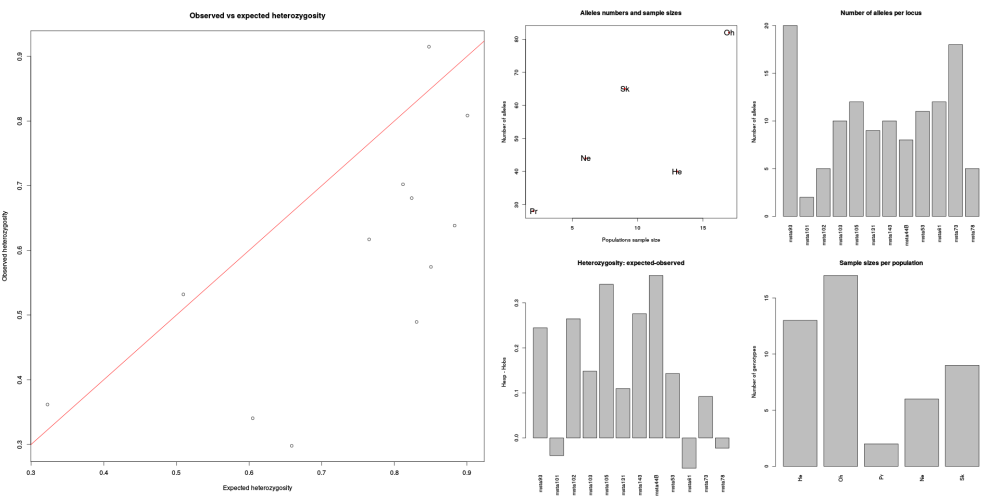
\includegraphics[width=\textwidth]{heterozygosity.png}
  \begin{spluscode}
    dev.off() # Closes graphical device - otherwise following
              # graphs would still be divided into 4 parts
  \end{spluscode}
\end{frame}

\begin{frame}[fragile]{Population statistics by poppr}
It returns various population statistics --- \textbf{png()} will produce set of figures for each population. You can similarly use \textbf{svg()}, \textbf{pdf()}, \ldots
  \begin{spluscode}
    png(filename="poppr_%03d.png", width=720, height=720, bg="white")
      # Output figures will be saved to the disk
    poppr(dat=hauss.genind, total=TRUE, sample=1000, method=4,
      missing="geno", cutoff=0.15, quiet=FALSE, clonecorrect=FALSE,
      hist=TRUE, minsamp=1, legend=TRUE)
    dev.off() # Closes graphical device - needed after use of functions
      # like png(), svg(), pdf(), ... to write the file(s) to the disk
  \end{spluscode}
  \begin{multicols}{2}
    \begin{itemize}
      \begin{tiny}
	\item Pop --- Population name (Note that ``Total'' also means ``Pooled'')
	\item N --- Number of individuals observed
	\item MLG --- Number of multilocus genotypes (MLG) observed
	\item eMLG --- The number of expected MLG at the smallest sample size ≥ 10 based on rarefaction
	\item SE --- Standard error based on eMLG
	\item H --- Shannon-Wiener Index of MLG diversity
	\item G --- Stoddart and Taylor's Index of MLG diversity
	\item Hexp --- Nei's 1978 genotypic diversity (corrected for sample size), or Expected Heterozygosity
	\item E.5 --- Evenness, E5
	\item Ia --- The index of association, IA
	\item rbarD --- The standardized index of association
	\item See \href{http://grunwaldlab.cgrb.oregonstate.edu/poppr-r-package-population-genetics/manual-documentation-news-and-changes}{poppr's manual} for details
      \end{tiny}
    \end{itemize}
  \end{multicols}
\end{frame}

\begin{frame}[fragile]{Departure from Hardy-Weinberg equilibrium}
  \begin{spluscode}
    # Departure from HWE
    hauss.hwe <- HWE.test.genind(x=hauss.genind, permut=TRUE,
      nsim=1000, res.type="matrix")
    # According to populations
    barplot(apply(X=hauss.hwe<0.05, 1, FUN=mean, na.rm=TRUE),
      las=3, ylab="Proportion of departure from HWE", main="By
      population", names.arg=hauss.genind@pop.names)
    # According to loci
    barplot(apply(X=hauss.hwe<0.05, 2, FUN=mean, na.rm=TRUE),
      las=3, ylab="Proportion of departure from HWE", main="By marker")
    hauss.hwe.test <- hw.test(x=hauss.loci, B=1000)
    hauss.hwe.test
    # List of lists for all combinations of loci and populations
    hauss.hwe.full <- HWE.test.genind(x=hauss.genind, permut=TRUE,
      nsim=1000, res.type="full")
    hauss.hwe.full # Very looong list...
  \end{spluscode}
\end{frame}

\begin{frame}[fragile]{Departure from HWE --- results}
  \begin{multicols}{2}
    \begin{footnotesize}
      > hauss.hwe.test
      \begin{tabular}{lllll}
	& chi\textasciicircum2 & df & Pr(chi\textasciicircum2 >) & Pr.exact\\
	msta93 & 383.5519728 & 190 & 3.552714e-15 & 0.000\\
	msta101 & 0.6927242 & 1 & 4.052393e-01 & 0.657\\
	msta102 & 83.0741964 & 10 & 1.250111e-13 & 0.000\\
	msta103 & 77.1819098 & 45 & 1.998865e-03 & 0.000\\
	msta105 & 282.3441356 & 66 & 0.000000e+00 & 0.000\\
	msta131 & 175.8647805 & 36 & 0.000000e+00 & 0.000\\
	msta143 & 155.4567196 & 45 & 4.474199e-14 & 0.000\\
	msta44B & 112.6283892 & 28 & 4.149125e-12 & 0.000\\
	msta53 & 110.2581985 & 55 & 1.436375e-05 & 0.002\\
	msta61 & 70.7719907 & 66 & 3.215148e-01 & 0.070\\
	msta73 & 310.9811293 & 153 & 7.842615e-13 & 0.000\\
	msta78 & 4.4688908 & 10 & 9.237260e-01 & 0.569
      \end{tabular}
    \end{footnotesize}
    \begin{flushright}
      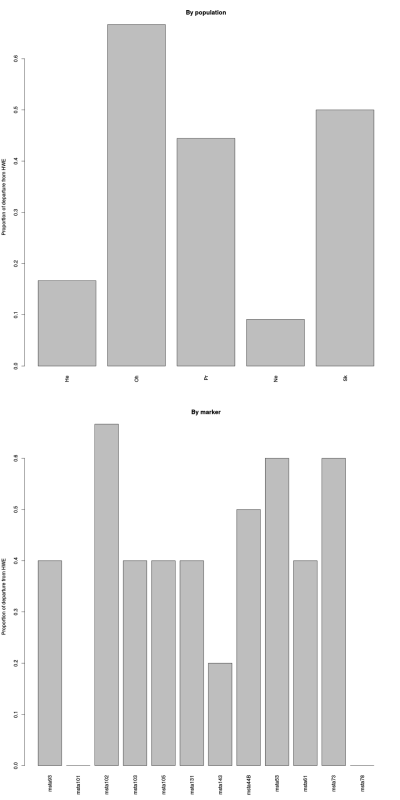
\includegraphics[height=6.5cm]{hwe.png}
    \end{flushright}
  \end{multicols}
\end{frame}

\begin{frame}[fragile]{F-statistics and population theta}
Functions return tables of Fst/thetas values for populations/loci
  \begin{spluscode}
    # Fit, Fst and Fis for each locus
    Fst(x=hauss.loci.cor, pop=1)
    # multilocus estimators of variance components and F-statistics,
    # alternative to Fst
    fstat(x=hauss.genind, pop=NULL, fstonly=FALSE)
    # Nei's pairwise Fst between all pairs of populations.
    # Difference in res.type="dist"/"matrix" is only in format of output
    pairwise.fst(x=hauss.genind, pop=NULL, res.type="matrix", truenames=T)
    # Estimates of population theta according to Kimmel et al. 1998
    theta.msat(hauss.loci.cor)
  \end{spluscode}
  \splus/Fst(x=hauss.loci.cor, pop=1)/
  \begin{tabular}{llll}
    & Fit & Fst & Fis\\
    msta93 & 0.31835291 & 0.17867087 & 0.17006829\\
    msta101 & -0.09968472 & 0.04064928 & -0.14628018\\
    \ldots & \ldots & \ldots & \ldots
  \end{tabular}
\end{frame}

\begin{frame}[fragile]{Multi locus genotypes}
  \begin{multicols}{2}
  \begin{spluscode}
    # Total number of MLGs
    # (simple value)
    mlg(pop=hauss.genind, quiet=FALSE)
    # MLGs shared among populations
    mlg.crosspop(pop=hauss.genind,
      df=TRUE, quiet=FALSE)
    # Detailed view on distribution
    # of MLGs into populations
    # (table and/or plot)
    mlg.table(pop=hauss.genind,
      bar=TRUE, total=TRUE,
      quiet=FALSE)
    # See manual pages for details
  \end{spluscode}
  \columnbreak
  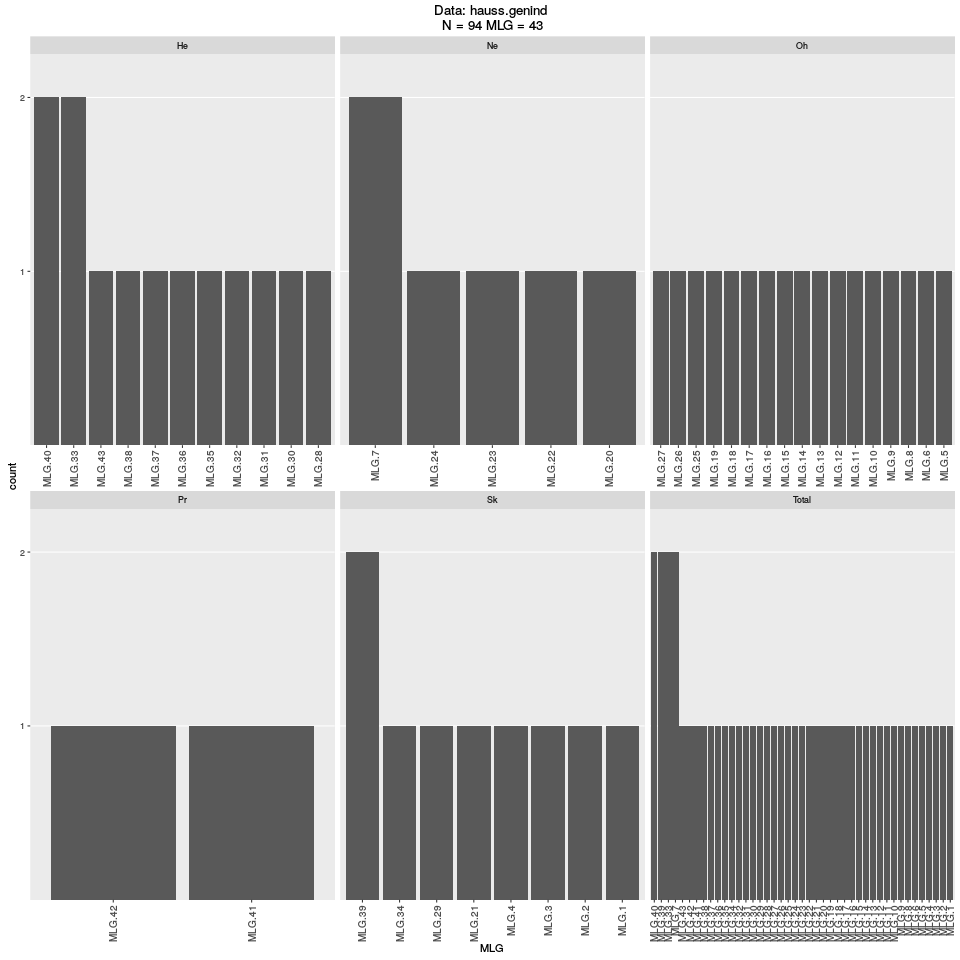
\includegraphics[height=6cm]{mlg.png}
  \end{multicols}
Functions from poppr package --- the best for microsatellites, although available also from another data types
\end{frame}

\subsection{Genetic distances}

\begin{frame}[fragile]{Basic distances}
  \begin{spluscode}
    # Euclidean distance for individuals
    hauss.dist <- dist(x=hauss.genind, method="euclidean", diag=T, upper=T)
    hauss.dist
    # Nei's distance (not Euclidean) for populations
    # (other methods are available, see ?dist.genpop)
    hauss.dist.pop <- dist.genpop(x=hauss.genpop, method=1, diag=T, upper=T)
    # Test if it is Euclidean
    is.euclid(hauss.dist.pop, plot=TRUE, print=TRUE, tol=1e-10) # FALSE = No
    # Turn to be Euclidean
    hauss.dist.pop <- cailliez(distmat=hauss.dist.pop, print=FALSE,
      tol=1e-07, cor.zero=TRUE)
    # Test if it is Euclidean
    is.euclid(hauss.dist.pop, plot=TRUE, print=TRUE, tol=1e-10) # TRUE = OK
    # Show it
    hauss.dist.pop
  \end{spluscode}
Most of analysis based on distances more or less require Euclidean (non-negative) distances. If the distance matrix contains non-Euclidean distances, the result can be weird\ldots
\end{frame}

\begin{frame}[fragile]{Distances reflecting microsatellite repeats}
  \begin{spluscode}
    # Bruvo's distances weighting SSRs repeats - take care about replen
    # parameter - requires repetition length for every SSRs locus
    hauss.dist.bruvo <- bruvo.dist(pop=hauss.genind, replen=rep(2, 12),
      loss=TRUE)
    # Test if it is Euclidean
    is.euclid(hauss.dist.bruvo, plot=TRUE, print=TRUE, tol=1e-10)
    # Turn to be Euclidean
    hauss.dist.bruvo <- cailliez(distmat=hauss.dist.bruvo, print=FALSE,
      tol=1e-07, cor.zero=TRUE)
    # Test if it is Euclidean
    is.euclid(hauss.dist.bruvo, plot=TRUE, print=TRUE, tol=1e-10)
    # Show it
    hauss.dist.bruvo
  \end{spluscode}
See poppr's manual and manual pages of the functions for details and different possibilities of settings.
\end{frame}

\begin{frame}{Turning distance matrix into Euclidean is controversial\ldots}
\begin{footnotesize}
  How to deal with zero distances in original matrix? There is no really good solution\ldots\\ Histograms of Bruvo distance before and after transformation:
\end{footnotesize}
\begin{center}
  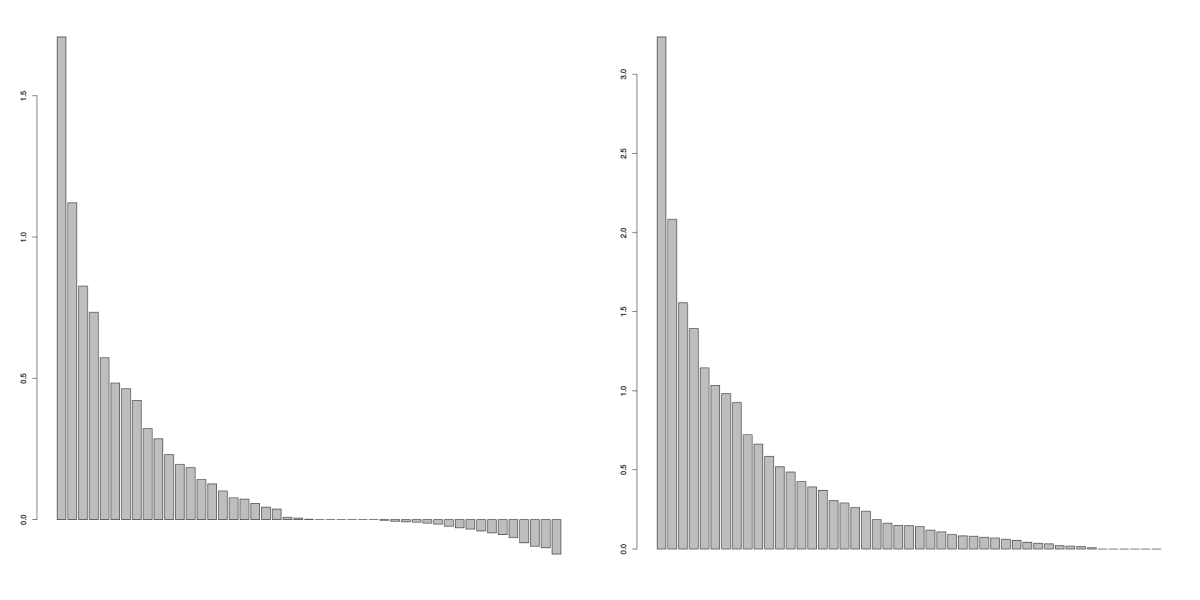
\includegraphics[width=\textwidth]{bruvodist.png}
\end{center}
\end{frame}

\begin{frame}[fragile]{More distances\ldots}
  \begin{spluscode}
    # Nei's distance (not Euclidean) for individuals
    # (other methods are available, see ?nei.dist from poppr package)
    hauss.dist.nei <- nei.dist(x=hauss.genind, warning=TRUE)
    hauss.dist.nei
    # Dissimilarity matrix returns a distance reflecting the number of
    # allelic differences between two individuals
    hauss.dist.diss <- diss.dist(x=hauss.genind, percent=FALSE, mat=TRUE)
    hauss.dist.diss
  \end{spluscode}
\vfil
Import own distance matrix from another software:
\begin{multicols}{2}
  \begin{footnotesize}
    \begin{verbatim}
   Fe       He      Oh      ...
Fe 0.00000  132.019 109.159 ...
He 132.0191 0.00000 9.89111 ...
Oh 109.1590 9.89111 0.00000 ...
Pr 139.5669 8.55312 4.40562 ...
Ne 156.7619 9.96143 16.6927 ...
... ...     ...     ...     ...
    \end{verbatim}
  \end{footnotesize}
  \columnbreak
  \begin{spluscode}
    MyDistance <- read.csv("distances.
      txt", header=TRUE, sep="\t",
      dec=".", row.names=1)
    MyDistance <- as.dist(MyDistance)
    class(MyDistance)
    dim(MyDistance)
    MyDistance
  \end{spluscode}
\end{multicols}
\end{frame}

\begin{frame}[fragile]{Distances among DNA sequences}
\alert{The sequences must be aligned before calculating distances among them!}
\vfill
  \begin{spluscode}
    ?dist.dna # There are various models available
    usflu.dist <- dist.dna(x=usflu.dna, model="TN93")
    usflu.dist
    class(usflu.dist)
    dim(as.matrix(usflu.dist))
    meles.dist <- dist.dna(x=meles.dna, model="F81")
    meles.dist
    class(meles.dist)
    dim(as.matrix(meles.dist))
  \end{spluscode}
\end{frame}

\begin{frame}[fragile]{Distances and genlight object}
Pairwise genetic distances for each data block (genlight objects with whole genome data) --- sensitive to missing data (not useful in every case):
\vfill
  \begin{spluscode}
    usflu.dists <- lapply(X=usflu.genlight, FUN=function(DDD)
      dist(as.matrix(DDD)))
    class(usflu.dists)
    names(usflu.dists)
    class(usflu.dists[[1]])
    usflu.distr <- Reduce(f="+", x=usflu.dists)
    class(usflu.distr)
    usflu.distr
    # It is possible to use just basic dist function on whole
    # genlight object
    usflu.distg <- dist(as.matrix(usflu.genlight))
  \end{spluscode}
\vfill
Rationale of this approach is to save resources when dividing whole data set into smaller blocks --- useful for huge data, nor for most of the cases
\end{frame}

\begin{frame}[fragile]{Visualize pairwise genetic similarities}
\begin{multicols}{2}
\vfil
  \begin{spluscode}
    # table.paint() requires data
    # frame, dist can't be directly
    # converted to DF
    table.paint(df=as.data.frame(
      as.matrix(usflu.dist)), cleg=0,
      clabel.row=0.5, clabel.col=0.5)
    # Same visualization, coloured
    # heatmap() reorders values
    # because by default it plots
    # also dendrograms on the edges
    heatmap(x=as.matrix(usflu.dist),
      Rowv=NA, Colv=NA, symm=TRUE)
  \end{spluscode}
\vfil
  Another possibility is to use function \textbf{corrplot()} from package \textbf{corrplot} --- it plots correlation plots.
\vfil
  \columnbreak
  \begin{center}
    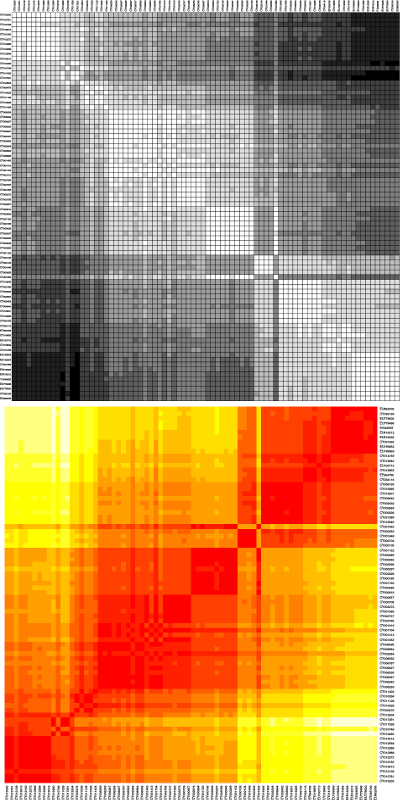
\includegraphics[height=6.5cm]{dna-dists.png}
  \end{center}
\end{multicols}
\end{frame}

\subsection{Hierarchical clustering}

\begin{frame}[fragile]{Heatmaps}
\begin{multicols}{2}
  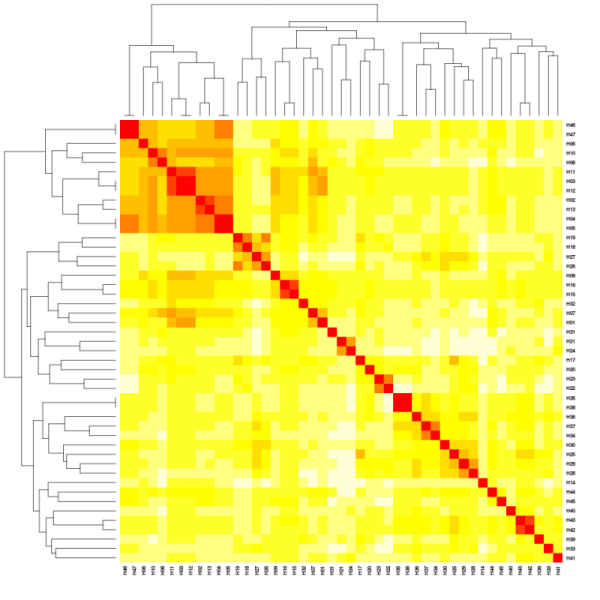
\includegraphics[height=6cm]{heatmap.png}
  \columnbreak
  \begin{spluscode}
    # Based on various distances
    heatmap(as.matrix(hauss.dist),
      symm=TRUE, labRow=rownames(
      as.matrix(hauss.dist.bruvo)),
      labCol=colnames(as.matrix(
      hauss.dist.bruvo)))
      # hauss.dist doesn't contain
      # names of individuals - add here
    heatmap(as.matrix(hauss.dist.pop),
      symm=TRUE)
    heatmap(as.matrix(hauss.dist.
      bruvo), symm=TRUE)
    heatmap(as.matrix(hauss.dist.
      diss), symm=TRUE)
  \end{spluscode}
\end{multicols}
\begin{footnotesize}
  There are various settings --- colours, dendrogram, \ldots See \textbf{?heatmap}.
\end{footnotesize}
\vfil
\end{frame}

\begin{frame}[fragile]{Hierarchical clustering --- UPGMA and others}
\begin{multicols}{2}
  \begin{spluscode}
    # According to distance used
    # see ?hclust for methods
    plot(hclust(d=hauss.dist,
      method="complete"))
    plot(hclust(d=hauss.dist.pop,
      method="complete"))
    plot(hclust(d=hauss.dist.
      bruvo, method="complete"))
  \end{spluscode}
This is very basic function to make dendrogram. There are better possibilities (NJ etc).
  \columnbreak
  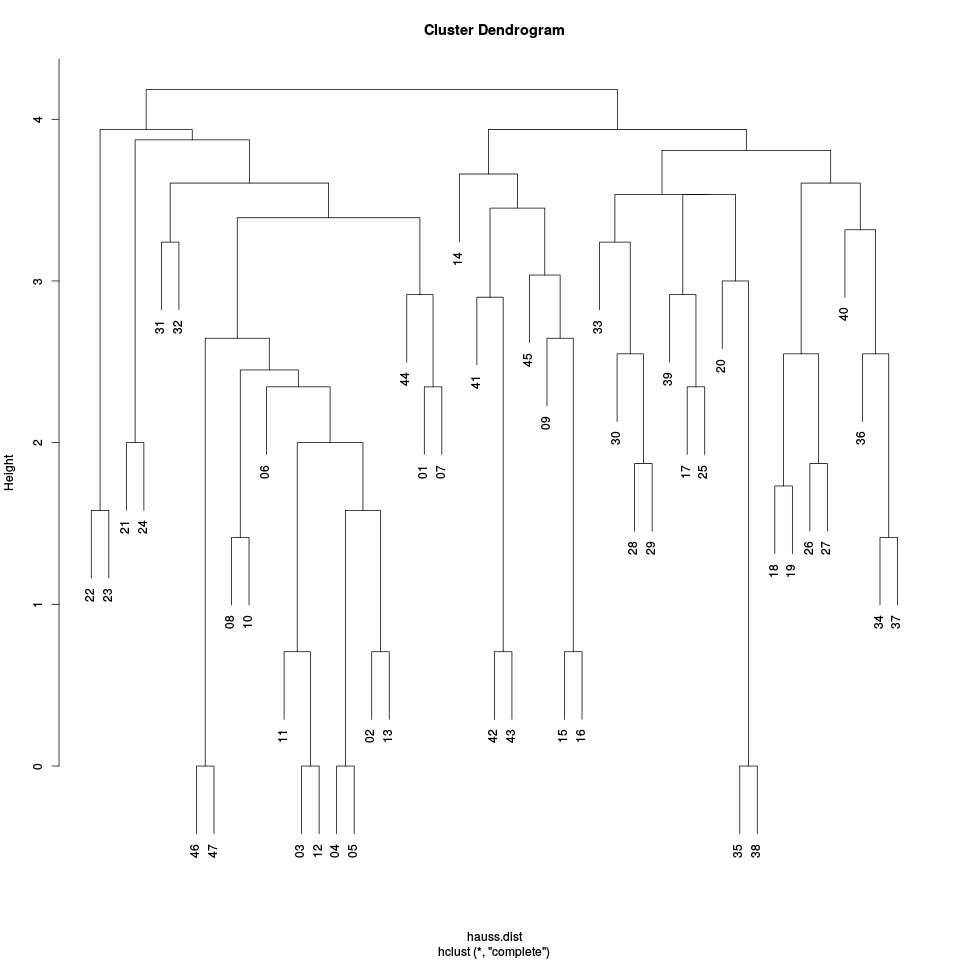
\includegraphics[height=6cm]{hierclust.png}
\end{multicols}
\end{frame}

\begin{frame}[fragile]{UPGMA and its test}
  \begin{spluscode}
    # Calculate it
    # Saving as phylo object (and not hclust) gives more
    # possibilities for further plotting and manipulations
    usflu.upgma <- as.phylo(hclust(d=usflu.dist, method="average"))
    plot.phylo(x=usflu.upgma, cex=0.75)
    title("UPGMA tree")
    # Test quality - tests correlation of original distance in the matrix
    # and reconstructed distance from hclust object
    plot(x=as.vector(usflu.dist), y=as.vector(as.dist(
      cophenetic(usflu.upgma))), xlab="Original pairwise distances",
      ylab="Pairwise distances on the tree", main="Is UPGMA
      appropriate?", pch=20, col=transp(col="black",
      alpha=0.1), cex=2)
    abline(lm(as.vector(as.dist(cophenetic(usflu.upgma)))~
      as.vector(usflu.dist)), col="red")
  \end{spluscode}
\end{frame}

\begin{frame}{UPGMA is not the best choice here\ldots}
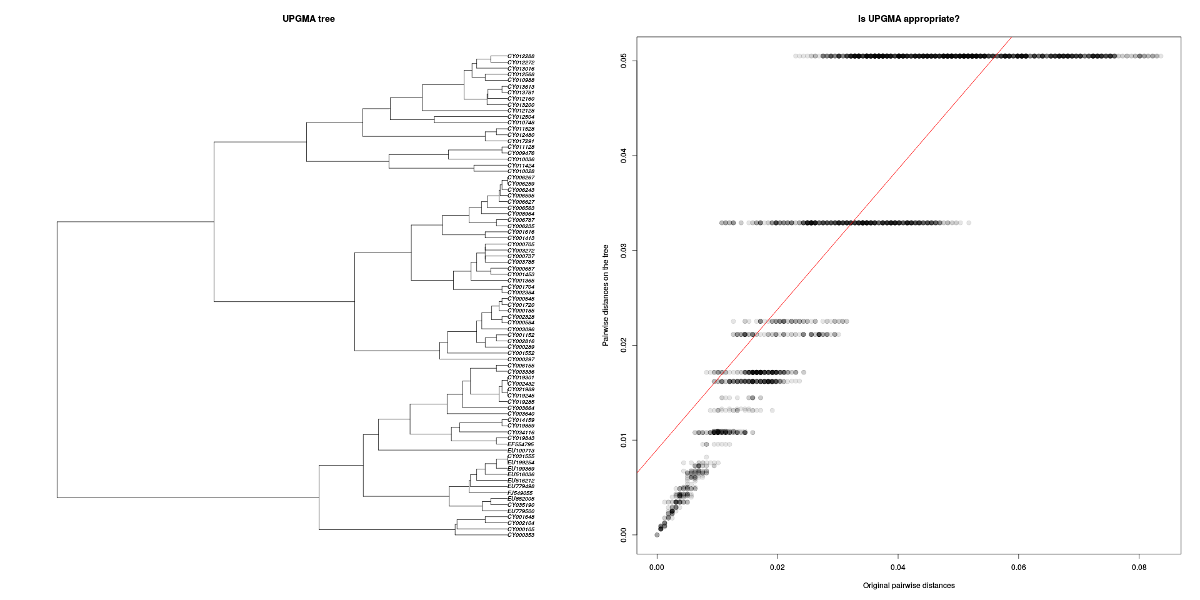
\includegraphics[width=\textwidth]{upgma.png}
\end{frame}

\subsection{AMOVA}

\begin{frame}[fragile]{AMOVA}
  \begin{spluscode}
    # From package pegas (doesn't directly show percentage of variance)
    hauss.pop <- hauss.genind$pop
    hauss.amova <- amova(hauss.dist~hauss.pop, data=NULL,
      nperm=1000, is.squared=TRUE)
    hauss.amova
    # Output:
    $tab
                   SSD      MSD df
    hauss.pop 15.11916 3.779790  4
    Error     59.62501 1.419643 42
    Total     74.74417 1.624873 46
    # Another possibility is poppr.amova - for more complicated hierarchy
    # see ?poppr.amova
  \end{spluscode}
\end{frame}

\subsection{MSN}

\begin{frame}[fragile]{Minimum Spanning Network}
\begin{multicols}{2}
  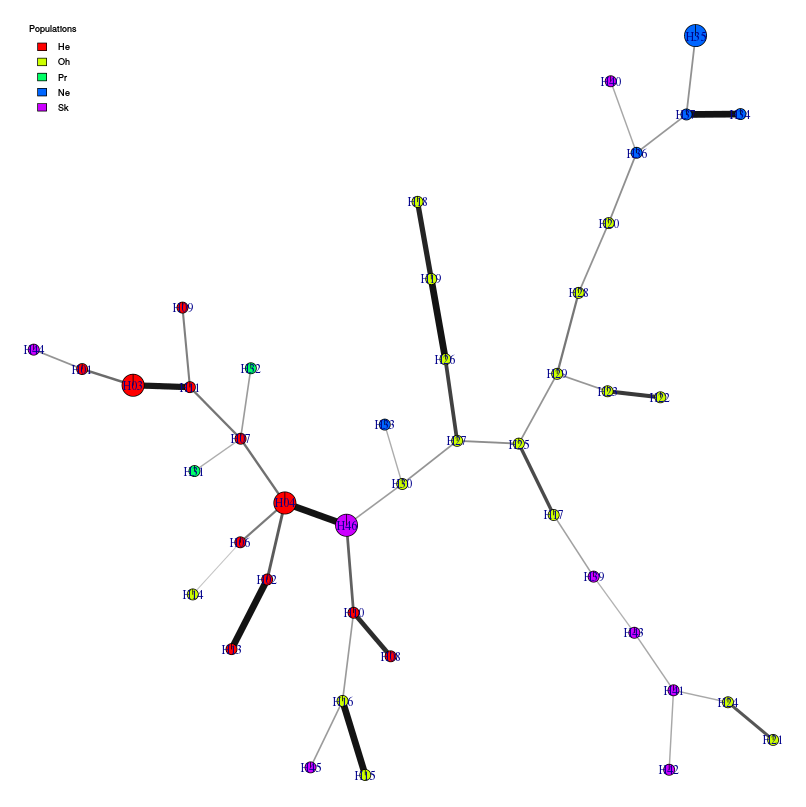
\includegraphics[height=6cm]{msn.png}
  \columnbreak
  \begin{spluscode}
    bruvo.msn(pop=hauss.genind,
      replen=rep(2, 12), loss=TRUE,
      palette=rainbow, vertex.label=
      "inds", gscale=TRUE,
      wscale=TRUE, showplot=TRUE)
  \end{spluscode}
  Package poppr, based on Bruvo's distance (for SSRs).
  \begin{center}
    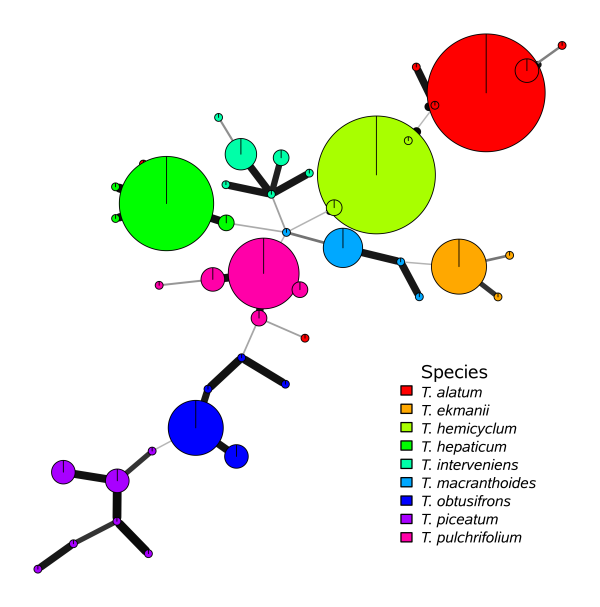
\includegraphics[width=3.5cm]{msn-bruvo_no_labels.png}
  \end{center}
\end{multicols}
\end{frame}

\subsection{NJ (and UPGMA) tree}

\begin{frame}[fragile]{Calculate and test NJ tree}
  \begin{spluscode}
    # Calculates the tree (try with various distances)
    hauss.nj <- nj(hauss.dist)
    # Test tree quality - plot original vs. reconstructed distance
    plot(as.vector(hauss.dist), as.vector(as.dist(cophenetic(hauss.nj))),
      xlab="Original distance", ylab="Reconstructed distance")
    abline(lm(as.vector(hauss.dist) ~
      as.vector(as.dist(cophenetic(hauss.nj)))), col="red")
    summary(lm(as.vector(hauss.dist) ~
      as.vector(as.dist(cophenetic(hauss.nj))))) # Prints summary text
    # Bootstrap
    hauss.boot <- boot.phylo(phy=hauss.nj, x=hauss.loci.cor,
      FUN=function(XXX) nj(dist(loci2genind(XXX))), B=1000)
    # Plot a basic tree - see ?plot.phylo for details
    plot.phylo(x=hauss.nj, type="phylogram")
    plot.phylo(x=hauss.nj, type="cladogram", edge.width=2)
    plot.phylo(x=hauss.nj, type="fan", edge.width=2, edge.lty=2)
    plot.phylo(x=hauss.nj, type="radial", edge.color="red",
      edge.width=2, edge.lty=3, cex=2)
  \end{spluscode}
\end{frame}

\begin{frame}{Choose your tree\ldots}
  \begin{center}
    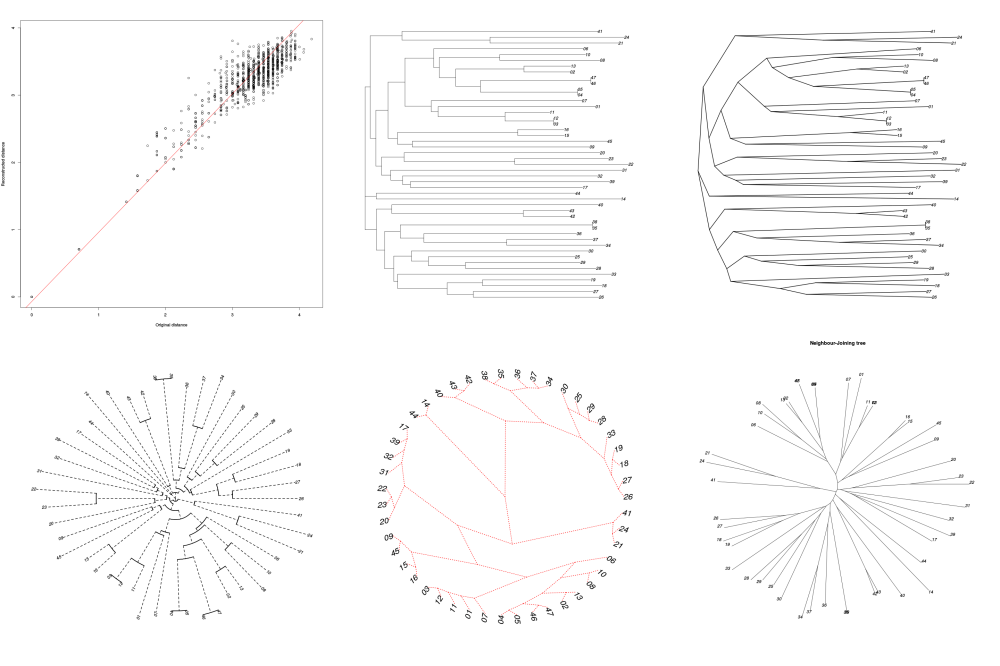
\includegraphics[width=\textwidth-1.5cm]{nj1.png}
  \end{center}
\end{frame}

\begin{frame}[fragile]{Nicer trees}
  \begin{footnotesize}
  \begin{spluscode}
    ## Plot a nice tree with colored tips
    plot.phylo(x=hauss.nj, type="unrooted", show.tip=F, lwd=3, main="NJ")
    # Labels for nodes - bootstrap - see ?nodelabels for graphical settings
    nodelabels(text=round(hauss.boot/10))
    # Colored labels - creates vector of colors according to populations
    nj.rainbow<-colorRampPalette(rainbow(length(levels(pop(hauss.genind)))))
    tiplabels(text=hauss.genind$ind.names, bg=fac2col(x=hauss.genind$pop,
      col.pal=nj.rainbow)) # Coloured tips
    ## Plot BW tree with tip symbols and legend
    plot.phylo(x=hauss.nj, type="cladogram", show.tip=F, lwd=3, main="NJ")
    axisPhylo() # Add axis with distances
    # From node labels let's remove unneeded frame
    nodelabels(text=round(hauss.boot/10), frame="none", bg="white")
    # As tip label we use only symbols - see ?points for graphical details
    tiplabels(frame="none", pch=rep(0:4,times=c(13,17,2,6,9)), lwd=2, cex=2)
    # Plot a legend explainindg symbols
    legend(x="topleft", legend=c("He", "Oh", "Pr", "Ne", "Sk"), 
      border="black", pch=0:4, pt.lwd=2, pt.cex=2, bty="o", bg="lightgrey",
      box.lwd=2, cex=1.2, title="Populations")
  \end{spluscode}
  \end{footnotesize}
\end{frame}

\begin{frame}{Choose your tree\ldots}
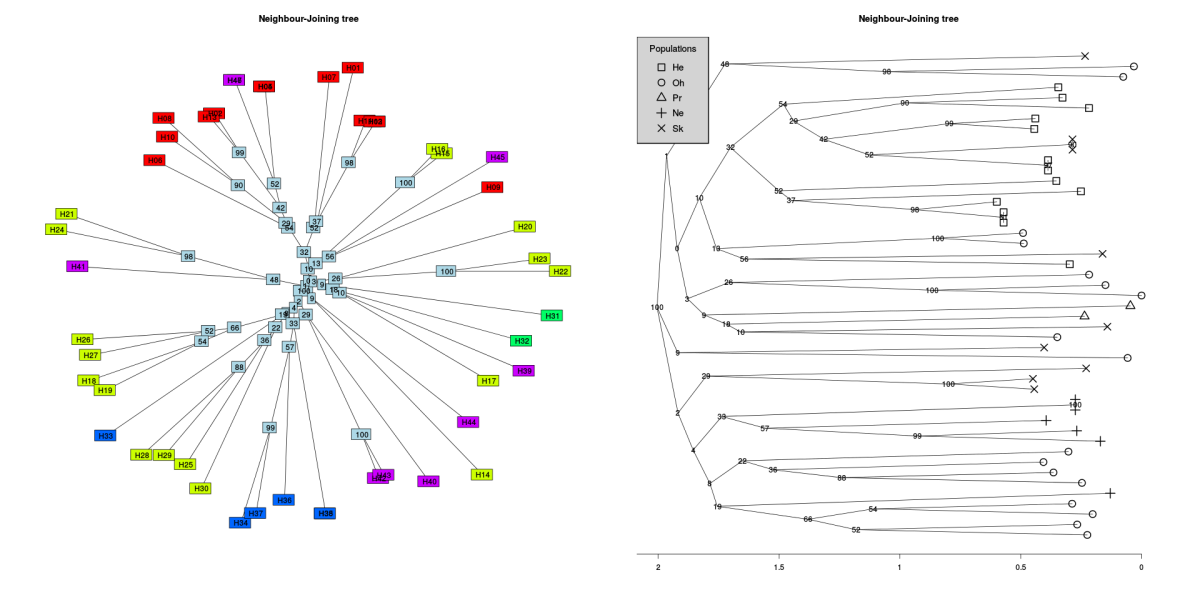
\includegraphics[width=\textwidth]{nj2.png}
\end{frame}

\begin{frame}[fragile]{Trees based on Bruvo's distance}
Package poppr (bootstrap is incorporated within the function)
  \begin{spluscode}
    # NJ
    hauss.nj.bruvo <- bruvo.boot(pop=hauss.genind, replen=rep(2, 12),
      sample=1000, tree="nj", showtree=TRUE, cutoff=1, quiet=FALSE)
    plot.phylo(x=hauss.nj.bruvo, type="unrooted", show.tip=FALSE,
      lwd=3, main="Neighbor-Joining tree.")
    # you can call node labels as phylo$node.labels or phylo[["node.labels"]]
    nodelabels(hauss.nj.bruvo[["node.labels"]]) 
    tiplabels(hauss.nj.bruvo[["tip.label"]], bg=fac2col(x=hauss.genind$pop,
      col.pal=nj.rainbow))
    # UPGMA
    hauss.upgma <- bruvo.boot(pop=hauss.genind, replen=rep(2, 12),
      sample=1000, tree="upgma", showtree=TRUE, cutoff=1, quiet=FALSE)
    plot.phylo(hauss.upgma, type="unrooted", show.tip=FALSE, lwd=3,
      main="UPGMA tree")
    nodelabels(hauss.upgma[["node.labels"]])
    tiplabels(hauss.upgma[["tip.label"]], bg=fac2col(x=hauss.genind@pop,
      col.pal=nj.rainbow))
  \end{spluscode}
\end{frame}

\begin{frame}{Choose your tree\ldots}
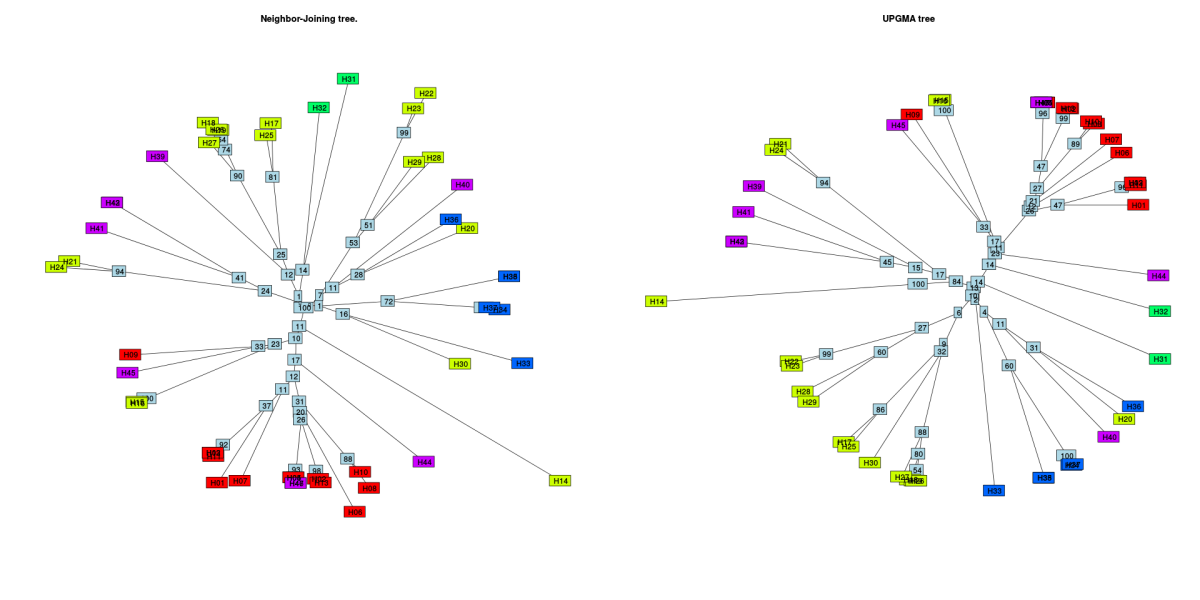
\includegraphics[width=\textwidth]{nj-upgma-bruvo.png}
\end{frame}

\begin{frame}[fragile]{NJ tree of populations}
  \begin{spluscode}
    # Populations
    hauss.nj.pop <- nj(hauss.dist.pop)
    # Bootstrap - source() loads external scripts
    # boot.phylo doesn't work for population trees
    source("http://trapa.cz/sites/default/rcourse/boot_phylo_nj_pop.r")
    hauss.boot.pop <- boot.phylo.nj.pop(hauss.nj.pop, hauss.genind, 1000)
    # Plot a tree
    plot(hauss.nj.pop, type="radial", cex=1.2, lwd=3,
      main="Neighbor-Joining tree of populations")
    # Labels - bootstrap
    nodelabels(round(hauss.boot.pop/10), frame="none")
    # Print information about phylo object
    print.phylo(hauss.nj.pop)
  \end{spluscode}
\end{frame}

\begin{frame}[fragile]{NJ tree based on DNA sequences}
  \begin{spluscode}
    usflu.tree <- nj(X=usflu.dist)
    # Plot it
    plot.phylo(x=usflu.tree, type="unrooted", show.tip=FALSE)
    title("Unrooted NJ tree")
    # Coloured tips
    usflu.pal <- colorRampPalette(topo.colors(length(levels(as.factor(
      usflu.annot[["year"])))))
    # Tip labels
    tiplabels(text=usflu.annot$year, bg=num2col(usflu.annot$year,
      col.pal=usflu.pal), cex=0.75)
    # Legend - describing years - pretty() automatically shows best
    # values from given range, num2col() selects colours from colour scale
    legend(x="bottomright", fill=num2col(x=pretty(x=1993:2008, n=8),
      col.pal=usflu.pal), leg=pretty(x=1993:2008, n=8), ncol=1)
  \end{spluscode}
\end{frame}

\begin{frame}[fragile]{Root the tree}
  \begin{spluscode}
    # Root the tree - "outgroup" is name of accession (in quotation
    # marks) or number (position within phy object)
    usflu.tree.rooted <- root(phy=usflu.tree, outgroup=1)
    # Plot it
    plot.phylo(x=usflu.tree.rooted, show.tip=FALSE, edge.width=2)
    title("Rooted NJ tree")
    # Labeling of tips
    tiplabels(text=annot$year, bg=transp(num2col(x=annot$year,
      col.pal=usflu.pal), alpha=0.7), cex=0.75, fg="transparent")
    # Add axis with phylogenetic distance
    axisPhylo()
    # Legend - describing years - pretty() automatically shows best
    # values from given range, num2col() selects colours from colour scale
    legend(x="topright", fill=num2col(x=pretty(x=1993:2008, n=8),
      col.pal=usflu.pal), leg=pretty(x=1993:2008, n=8), ncol=1)
  \end{spluscode}
\end{frame}

\begin{frame}[fragile]{Bootstrap rooted tree}
  \begin{spluscode}
    # Calculate it
    usflu.boot <- boot.phylo(phy=usflu.tree.rooted, x=usflu.dna,
      FUN=function(EEE) root(nj(dist.dna(EEE, model="TN93")),
      outgroup=1), B=1000)
    # Plot the tree
    plot.phylo(x=usflu.tree.rooted, show.tip=FALSE, edge.width=2)
    title("NJ tree + bootstrap values")
    tiplabels(frame="none", pch=20, col=transp(num2col(x=annot[["year"]],
      col.pal=usflu.pal), alpha=0.7), cex=3.5, fg="transparent")
    axisPhylo()
    # Legend - describing years - pretty() automatically shows best
    # values from given range, num2col() selects colours from colour scale
    legend(x="topright", fill=num2col(x=pretty(x=1993:2008, n=8),
      col.pal=usflu.pal), leg=pretty(x=1993:2008, n=8), ncol=1)
    # Plots bootstrap support - note usflu.boot contains raw numbers
    # transform it into percent
    nodelabels(text=round(usflu.boot/10), cex=0.75)
  \end{spluscode}
\end{frame}

\begin{frame}[fragile]{Collapse branches with low bootstrap support}
  \begin{spluscode}
    usflu.tree.temp <- usflu.tree.rooted
    # Determine branches with low support - note BS values are in raw
    # numbers - use desired percentage with respect to number of bootstraps
    usflu.tocollapse <- match(x=which(usflu.boot < 700)+
      length(usflu.tree.rooted$tip.label), table=usflu.tree.temp$edge[,2])
    # Set length of bad branches to zero
    usflu.tree.temp$edge.length[usflu.tocollapse] <- 0
    # Create new tree
    usflu.tree.collapsed <- di2multi(phy=usflu.tree.temp, tol=0.00001)
    # Plot the consensus tree
    plot.phylo(x=usflu.tree.collapsed, show.tip=FALSE, edge.width=2)
    title("NJ tree after collapsing weak nodes")
    tiplabels(text=annot$year, bg=transp(num2col(x=annot[["year"]],
      col.pal=usflu.pal), alpha=0.7), cex=0.5, fg="transparent")
    axisPhylo()
    legend(x="topright", fill=num2col(x=pretty(x=1993:2008, n=8),
      col.pal=usflu.pal), leg=pretty(x=1993:2008, n=8), ncol=1)
  \end{spluscode}
\end{frame}

\begin{frame}{The trees}
  \begin{center}
    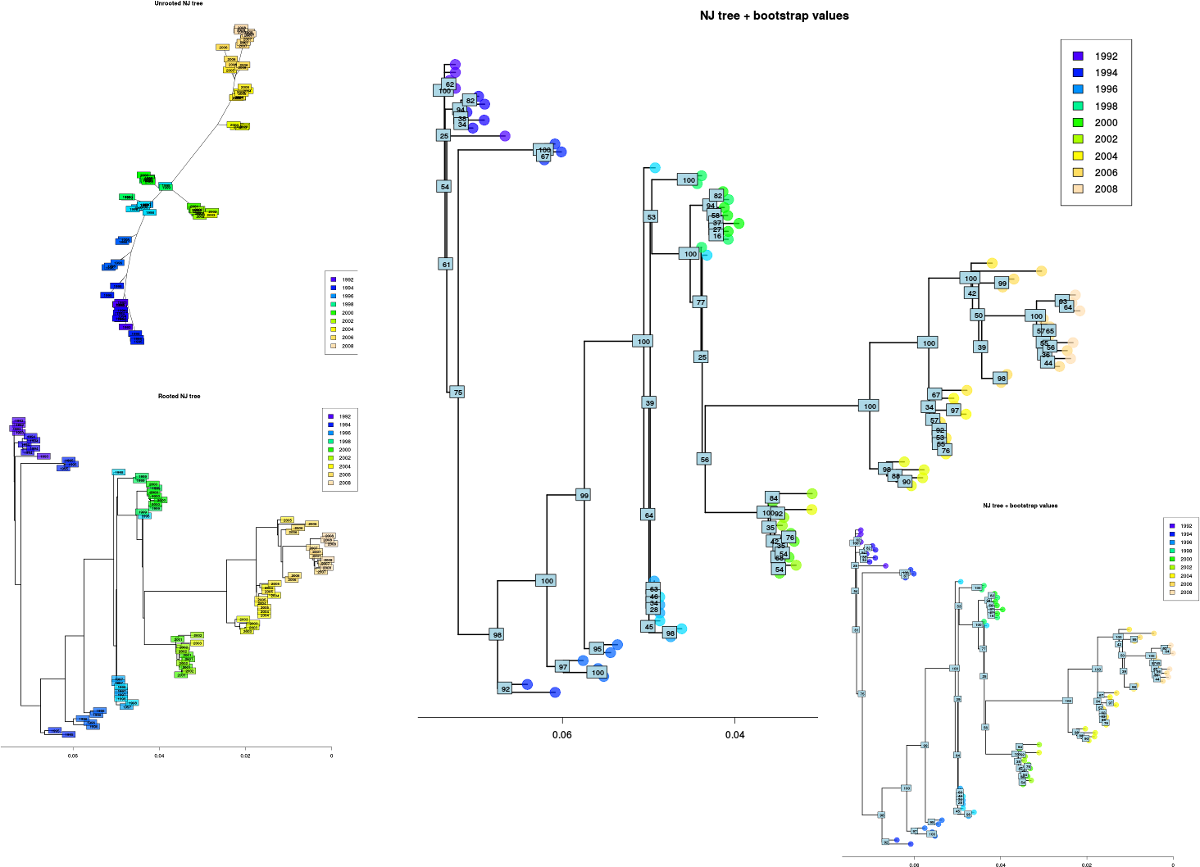
\includegraphics[width=\textwidth-2.5cm]{nj_dna.png}
  \end{center}
\end{frame}

\begin{frame}{NJ is death. Long live NJ!}
  \begin{itemize}
  \item ``Basic'' NJ has many limitations -- there are several tries to overcome them
  \item Package \textbf{phangorn} has functions \textbf{NJ()} and unweighted version \textbf{UNJ()}
  \item Package \textbf{ape} has functions \textbf{njs()} and \textbf{bionjs()} which are designed to perform well on distances with (more) missing values
  \item Function \textbf{bionj()} from \textbf{ape} implements BIONJ algorithm
  \item FastME functions (package \textbf{ape}) perform the minimum evolution algorithm and aim to be replacement of NJ --- read \textbf{?fastme} before use
  \item All those functions read distance matrix and their use is same as with ``classical'' \textbf{nj()} (read manual pages before using them) --- it is also from package \textbf{ape}
  \end{itemize}
\end{frame}

\subsection{PCoA}

\begin{frame}[fragile]{PCoA I}
  \begin{spluscode}
    hauss.pcoa <- dudi.pco(d=dist(x=scaleGen(x=hauss.genind, center=TRUE,
      scale=FALSE, truenames=TRUE, missing="NA"), method="euclidean"),
      scannf=FALSE, nf=3)
    # Basic display
    s.label(dfxy=hauss.pcoa$li, clabel=0.75)
    # To plot different axes use for example dfxy=hauss.pcoa$li[c(2, 3)]
    # Add kernel density
    s.kde2d(dfxy=hauss.pcoa$li, cpoint=0, add.plot=TRUE)
    # Adds histogram of Eigenvalues
    add.scatter.eig(w=hauss.pcoa$eig, nf=3, xax=1, yax=2,
      posi="bottomleft", sub="Eigenvalues")
    # Colored display according to populations
    # Creates vector of colors according to populations
    hauss.pcoa.col <- rainbow(length(levels(pop(hauss.genind))))
    s.class(dfxy=hauss.pcoa$li, fac=pop(hauss.genind), col=hauss.pcoa.col)
    add.scatter.eig(w=hauss.pcoa$eig, nf=3, xax=1, yax=2,
      posi="bottomleft", sub="Eigenvalues")
    title("Principal Coordinates Analysis") # Adds title to the graph
  \end{spluscode}
\end{frame}

\begin{frame}[fragile]{PCoA II}
\begin{multicols}{2}
  \begin{center}
    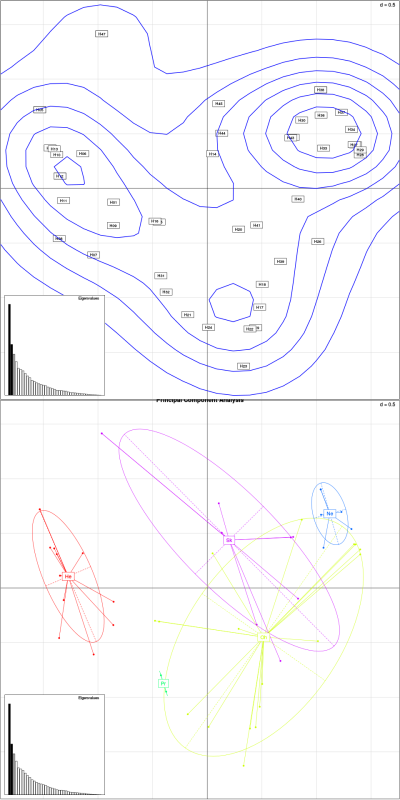
\includegraphics[height=6.5cm]{pcoa.png}
  \end{center}
  \columnbreak
  \begin{spluscode}
    hauss.pcoa.bruvo <- dudi.pco(d=	
      bruvo.dist(pop=hauss.genind,
      replen=rep(2, 12)), scannf=F,
      nf=3)
    s.class(dfxy=hauss.pcoa.bruvo$li,
      fac=pop(hauss.genind),
      col=hauss.pcoa.col)
    add.scatter.eig(hauss.pcoa.bruvo$
      eig, posi="bottomright", 3,1,2)
    # Another possibility for coloured
    # plot (see ?colorplot for details)
    colorplot(xy=hauss.pcoa$li[c(1, 2)],
      X=hauss.pcoa$li, transp=TRUE,
      cex=3, xlab="PC 1", ylab="PC 2")
    title(main="PCoA, axes 1 and 3")
    abline(v=0, h=0, col="grey", lty=2)
  \end{spluscode}
\end{multicols}
\end{frame}

\begin{frame}{PCoA --- Bruvo and colorplot}
  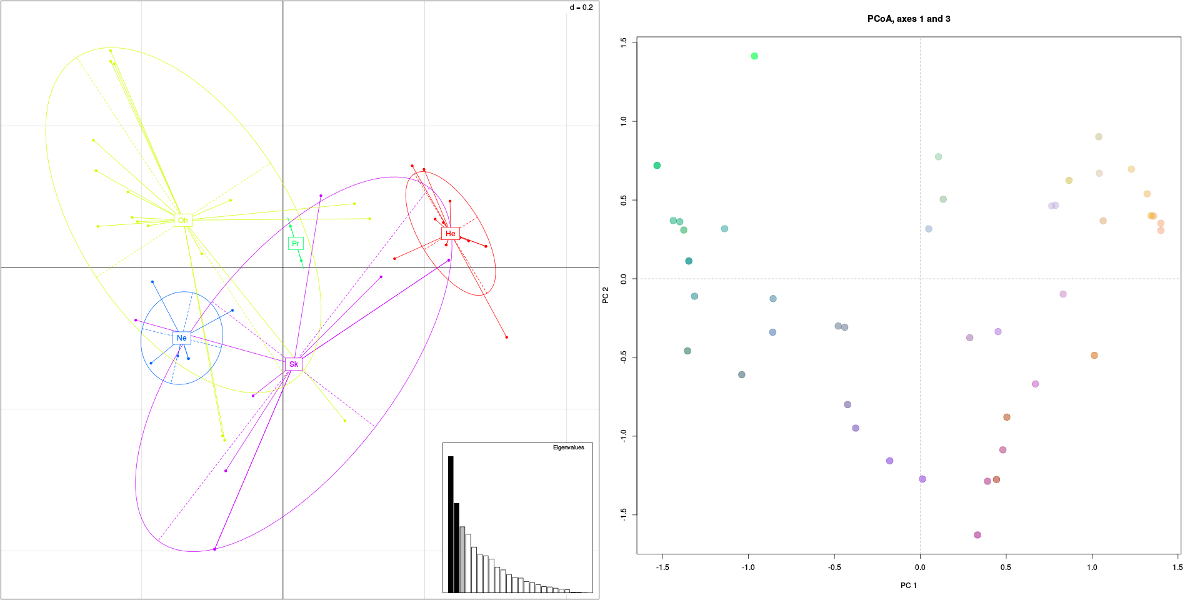
\includegraphics[width=\textwidth]{pcoa-dalsi.png}
\end{frame}

\section{DAPC}

\begin{frame}{DAPC}
\begin{itemize}
 \item Discriminant Analysis of Principal components
 \item Runs K-means Bayesian clustering on data transformed with PCA (reduces number of variables, speeds up process)
 \item Finally it runs discriminant analysis
 \item Various modes of displaying of results --- ``Structure-like'', ``PCA-like'' and more
 \item More information at \href{http://adegenet.r-forge.r-project.org/}{http://adegenet.r-forge.r-project.org/} and \textbf{adegenetTutorial("dapc")}
 \item If following commands would seem to complicated to you, try web interface by this command:
\end{itemize}
\splus/adegenetServer("DAPC")/
\end{frame}

\begin{frame}[fragile]{K-find --- Bayesian K-means clustering}
  \begin{spluscode}
    # Retain all informative PC (here about 35).
    # According to second graph select best K (here 2 or 3).
    hauss.kfind <- find.clusters(x=hauss.genind, stat="BIC",
      choose.n.clust=TRUE, max.n.clust=10, n.iter=100000, n.start=100,
      scale=FALSE, truenames=TRUE)
    # See results as text
    table(pop(hauss.genind), hauss.kfind$grp)
    hauss.kfind
    # Graph showing table of original and inferred populations and
    # assignment of individuals
    table.value(df=table(pop(hauss.genind), hauss.kfind$grp),
      col.lab=paste("Inferred\ncluster", 1:length(hauss.kfind$size)), grid=T)
    # For K=3 - note parameters n.pca and n.clust - we just rerun the
    # analysis and when results are stable, no problem here
    hauss.kfind3 <- find.clusters(x=hauss.genind, n.pca=35, n.clust=3,
      stat="BIC", choose.n.clust=FALSE, max.n.clust=10, n.iter=100000,
      n.start=100, scale=FALSE, truenames=TRUE)
  \end{spluscode}
\end{frame}

\begin{frame}[fragile]{K-find outputs}
\begin{multicols}{2}
  \begin{spluscode}
    # See results as text
    table(pop(hauss.genind),
      hauss.kfind3$grp)
    hauss.kfind3
    # Graph showing table of original
    # and inferred populations and
    # assignment of individuals
    table.value(
      df=table(pop(hauss.
      genind), hauss.kfind3$grp),
      col.lab=paste("Inferred\n
      cluster",
      1:length(hauss.kfind3$size)),
      grid=TRUE)
  \end{spluscode}
  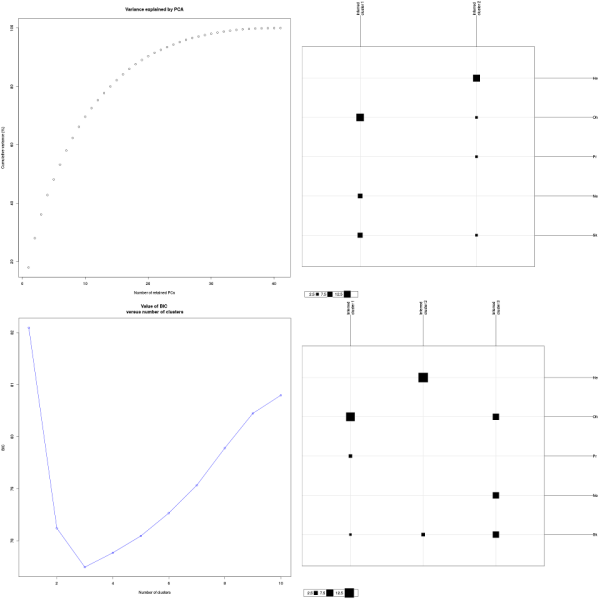
\includegraphics[height=6cm]{kmeans.png}
\end{multicols}
\end{frame}

\begin{frame}[fragile]{DAPC code I}
  \begin{spluscode}
    ## K=2
    # Creates DAPC
    # Number of informative PC (Here 15, adegenet recommends < N/3). Select
    # number of informative DA (here only one is available - no PCA graph)
    hauss.dapc <- dapc(x=hauss.genind, pop=hauss.kfind$grp, center=TRUE,
      scale=FALSE, var.contrib=TRUE, pca.info=TRUE, truenames=TRUE)
    # Information
    hauss.dapc
    # Density functions
    scatter(x=hauss.dapc, xax=1, yax=1, main="DAPC", bg="white", solid=0.5,
      leg=TRUE, txt.leg=c("Group 1", "Group 2"), posi.leg="topright")
    # Assignment of individuals to clusters
    assignplot(x=hauss.dapc)
    # Structure-like plot
    compoplot(x=hauss.dapc, xlab="Individuals", leg=FALSE)
    # Loadingplot - alleles the most adding to separation of individuals
    loadingplot(x=hauss.dapc$var.contr)
  \end{spluscode}
\end{frame}

\begin{frame}{DAPC for K=2}
\begin{center}
  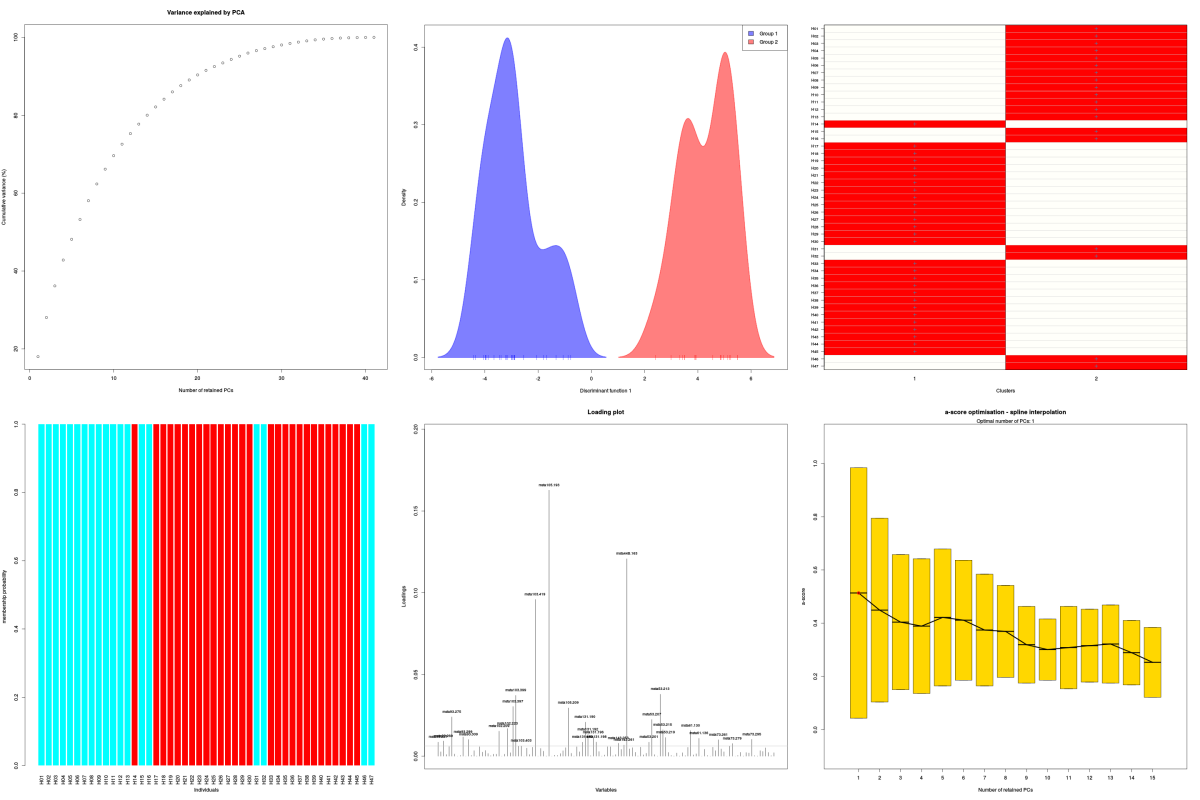
\includegraphics[width=\textwidth-1.5cm]{dapc2.png}
\end{center}
\end{frame}

\begin{frame}[fragile]{DAPC code II}
  \begin{spluscode}
    ## alfa-score - according to number of PC axis
    optim.a.score(x=hauss.dapc)
    # K=3
    # Creates DAPC
    # Number of informative PC (Here 15, adegenet recommends < N/3).
    # Select number of informative DA (here 2).
    hauss.dapc3 <- dapc(x=hauss.genind, pop=hauss.kfind3$grp, center=TRUE,
      scale=FALSE, var.contrib=TRUE, pca.info=TRUE, truenames=TRUE)
    # Information
    hauss.dapc
    # A la PCA graph
    scatter(x=hauss.dapc3, main="DAPC, Cardamine", bg="white", cex=3,
      clab=0, col=rainbow(3), posi.da="bottomleft", scree.pca=TRUE, 
      posi.pca="bottomright", leg=TRUE, txt.leg=c("Group 1", "Group 2",
      "Group 3"), posi.leg="topleft")
  \end{spluscode}
Especially graphical parameters have huge possiilities\ldots
\end{frame}

\begin{frame}{DAPC for K=3}
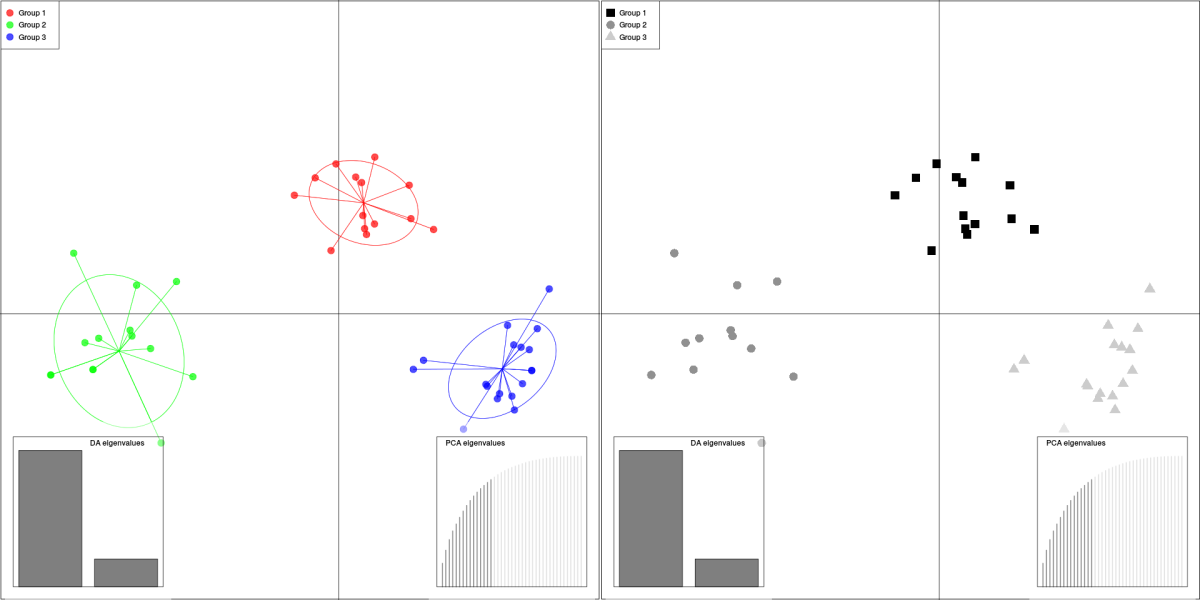
\includegraphics[width=\textwidth]{dapc3.png}
\end{frame}

\begin{frame}[fragile]{DAPC code III}
  \begin{spluscode}
    # Same in BW
    scatter(x=hauss.dapc3, main="DAPC, Cardamine", bg="white", pch=c(15:17),
      cell=0, cstar=0, solid=1, cex=2.5, clab=0, col=grey.colors(3, start=0,
      end=0.8, gamma=2, alpha=0), posi.da="bottomleft", scree.pca=TRUE,
      posi.pca="bottomright", leg=TRUE, txt.leg=c("Group 1", "Group 2",
      "Group 3"), posi.leg="topleft")
    # Density functions
    scatter(x=hauss.dapc3, xax=1, yax=1, main="DAPC", bg="white", solid=0.5,
      leg=T, txt.leg=c("Group 1", "Group 2", "Group 3"), posi.leg="topleft")
    # Assignment of individuals to clusters
    assignplot(hauss.dapc3)
    # Structure-like plot
    compoplot(hauss.dapc3, xlab="Individuals", leg=FALSE)
    # Loadingplot - alleles the most adding to separation of individuals
    loadingplot(hauss.dapc3$var.contr)
    # alfa-score - according to number of PC axis
    optim.a.score(hauss.dapc3)
  \end{spluscode}
\end{frame}

\begin{frame}{DAPC for K=3, extra information}
\begin{center}
  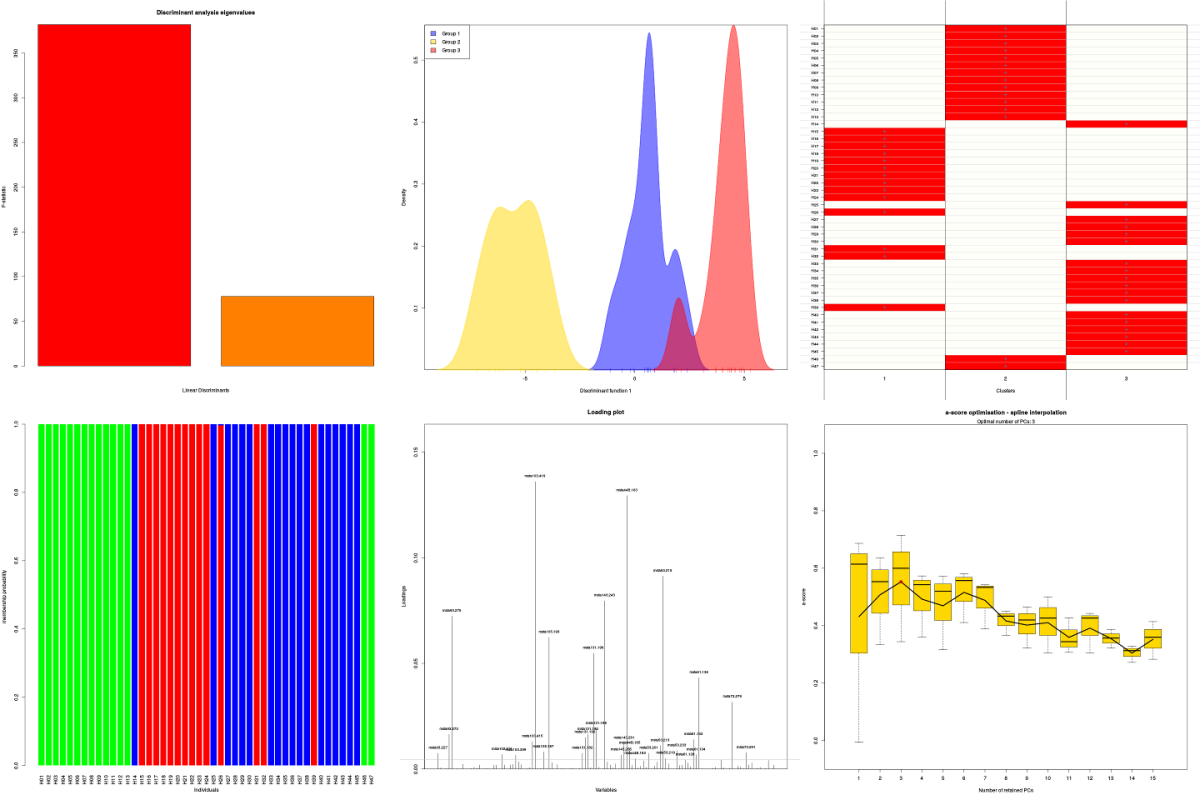
\includegraphics[width=\textwidth-1.5cm]{dapc3-extra.png}
\end{center}
\end{frame}

\begin{frame}{Another DAPC example}
\begin{center}
  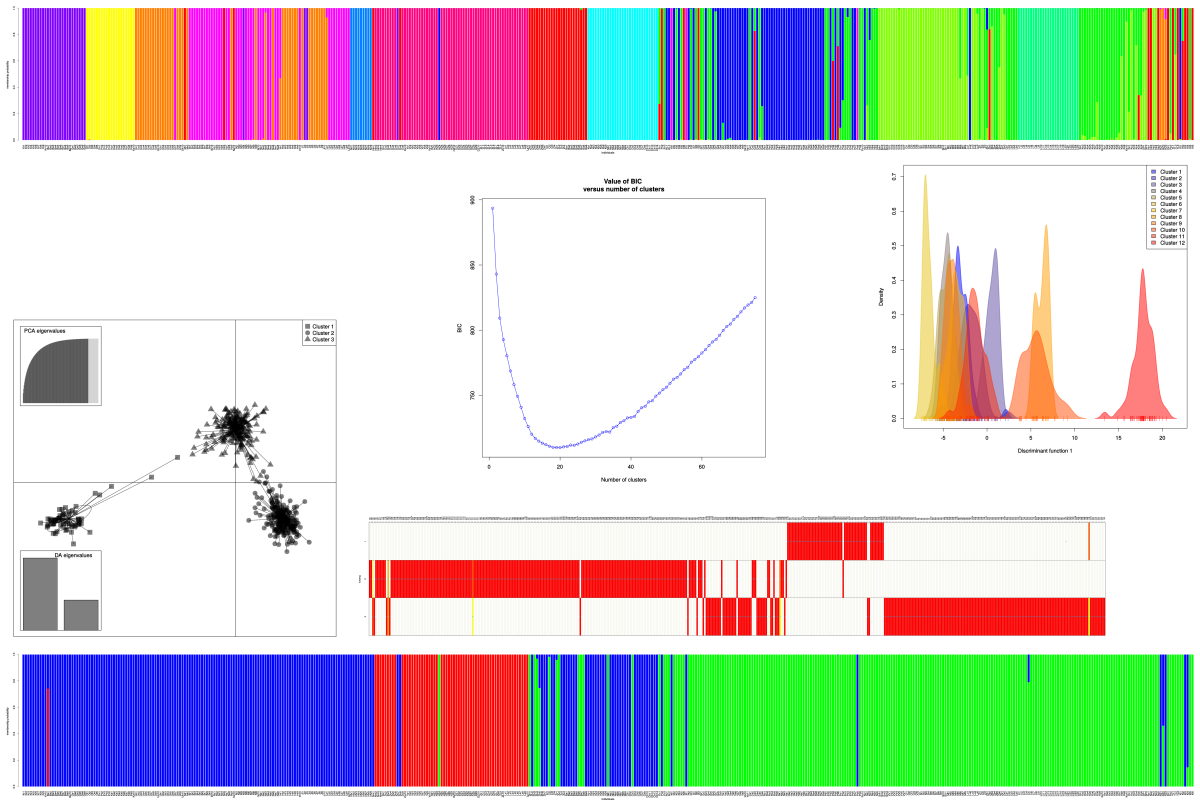
\includegraphics[width=\textwidth-1.5cm]{dapc.png}
\end{center}
\end{frame}

\section{SNP}

\begin{frame}[fragile]{Some functions to work with huge SNP data sets}
  \begin{spluscode}
    # Plot of missing data (white) and number of 2nd alleles
    glPlot(x=usflu.genlight, legend=TRUE, posi="topleft")
    # Sum of the number of second allele in each SNP
    usflu.freq <- glSum(usflu.genlight)
    # Plot distribution of (second) allele frequencies
    hist(x=usflu.freq, proba=TRUE, col="gold", xlab="Allele
      frequencies", main="Distribution of (second) allele frequencies")
    lines(x=density(usflu.freq)$x, y=density(usflu.freq)$y*1.5,
      col="red", lwd=3 )
    # Mean number of second allele in each SNP
    usflu.mean <- glMean(usflu.genlight)
    usflu.mean <- c(usflu.mean, 1-usflu.mean)
    # Plot distribution of allele frequencies
    hist(x=usflu.mean, proba=TRUE, col="darkseagreen3",
      xlab="Allele frequencies", main="Distribution of allele
      frequencies", nclass=20)
    lines(x=density(usflu.mean, bw=0.05)$x, y=density(usflu.mean,
      bw=0.05)$y*2, lwd=3)
  \end{spluscode}
\end{frame}

\begin{frame}[fragile]{Number of missing values in each locus}
  \begin{spluscode}
    # Play with bw parameter to get optimal image
    usflu.na.density <- density(glNA(usflu.genlight), bw=10)
    # Set range of xlim parameter from 0 to the length
    # of original alignment
    plot(x=usflu.na.density, type="n", xlab="Position in the alignment",
      main="Location of the missing values (NA)", xlim=c(0, 1701))
    polygon(c(usflu.na.density$x, rev(usflu.na.density$x)),
      c(usflu.na.density$y, rep(0, length(usflu.na.density$x))),
      col=transp("blue", alpha=0.3))
    points(glNA(usflu.genlight), rep(0, nLoc(usflu.genlight)), 
      pch="|", cex=2, col="blue")
  \end{spluscode}
\vfill
Those tools are designed mainly for situation when having multiple (nearly) complete genomes. It is not needed for smaller (normal) datasets. Lets keep hoping in fast development of computers\ldots
\end{frame}

\begin{frame}{Basic information about SNP: distribution of 2$^{nd}$ allele frequencies, missing data and number of 2$^{nd}$ allele, distribution of allele frequencies, and number of missing values in each locus}
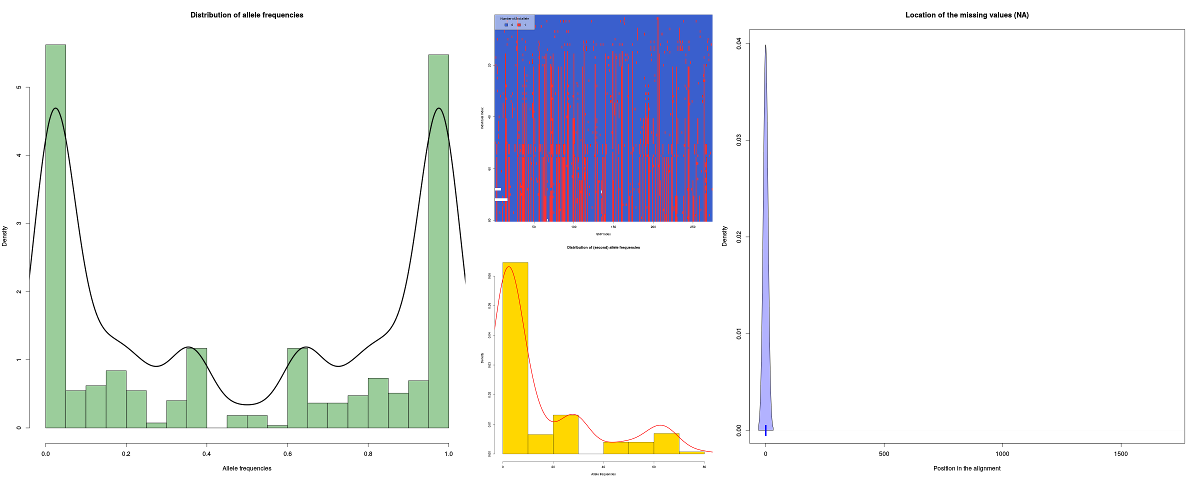
\includegraphics[width=\textwidth]{flu_alleles.png}
\end{frame}

\subsection{PCA and NJ}

\begin{frame}[fragile]{PCA, NJ and genlight objects}
  \begin{spluscode}
    usflu.pca <- glPca(x=usflu.genlight, center=TRUE, scale=FALSE,
      loadings=TRUE) # Select number of retained PC axes, about 10 here
    # Plot PCA
    scatter.glPca(x=usflu.pca, posi="bottomright")
    title("PCA of the US influenza data")
    # Coloured plot
    colorplot(usflu.pca$scores, usflu.pca$scores, transp=TRUE, cex=4)
    title("PCA of the US influenza data")
    abline(h=0, v=0, col="grey")
    add.scatter.eig(usflu.pca[["eig"]][1:40], 2, 1, 2, posi="topright",
      inset=0.05, ratio=0.3)
    # Calculate phylogenetic tree
    usflu.tree.genlight <- nj(dist(as.matrix(usflu.genlight)))
    # Plot coloured phylogenetic tree
    plot.phylo(x=usflu.tree.genlight, typ="fan", show.tip=FALSE)
    tiplabels(pch=20, col=usflu.col, cex=4)
    title("NJ tree of the US influenza data")
  \end{spluscode}
\end{frame}

\begin{frame}{PCA, NJ and genlight objects}
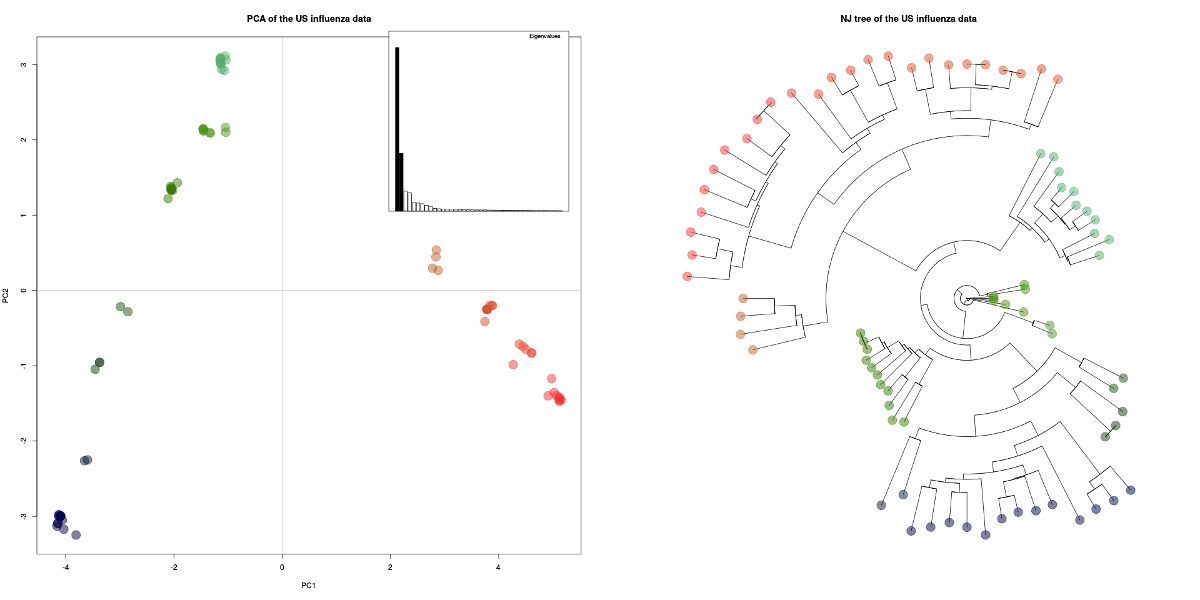
\includegraphics[width=\textwidth]{flu_pcoa_nj.png}
\end{frame}

\section{Spatial analysis}

\begin{frame}{Short overview of spatial genetics (in R)}
\begin{itemize}
  \item Basic approaches
  \begin{itemize}
    \item Moran's~\textit{I} --- several implementations (here as basic autocorrelation index, in sPCA and in Monmonier's algorithm), generally it is autocorrelation coefficient with broader use
    \item Mantel test --- several implementations, popular, although recently criticised as biologically irrelevant, generally correlation of two matrices (here genetic and geographical)
    \item Bayesian clustering using geographical information as a proxy and showing results in geographical context (here as implemented in Geneland)
    \item There are unlimited possibilities with connections with GIS software --- check specialised courses and literature
  \end{itemize}
\end{itemize}
\end{frame}

\subsection{Moran's~I}

\begin{frame}[fragile]{Calculation of Moran's \textit{I} I}
  \begin{spluscode}
    # Creates connection network
    hauss.connectivity <- chooseCN(xy=hauss.genind$other$xy, type=5,
      d1=0, d2=1, plot.nb=TRUE, result.type="listw", edit.nb=FALSE)
    hauss.connectivity
    # Output:
    Characteristics of weights list object:
    Neighbour list object:
    Number of regions: 47
    Number of nonzero links: 1120
    Percentage nonzero weights: 50.70167
    Average number of links: 23.82979
    Weights style: W
    Weights constants summary:
       n   nn S0       S1      S2
    W 47 2209 47 4.033607 207.037
    ###
  \end{spluscode}
\end{frame}

\begin{frame}[fragile]{Calculation of Moran's \textit{I} II}
  \begin{spluscode}
    # Test of Moran's I for 1st PCoA axis
    # Results can be checked against permuted values of moran.mc()
    moran.test(x=hauss.pcoa$li[,1], listw=hauss.connectivity,
      alternative="greater", randomisation=TRUE)
    # Output:
    Moran's I test under randomisation
    data:  hauss.pcoa$li[, 1]  
    weights: hauss.connectivity  
    Moran I statistic standard deviate = -18.514, p-value = 1
    alternative hypothesis: greater
    sample estimates:
    Moran I statistic       Expectation          Variance
        -0.5232003724     -0.0217391304      0.0007336276
    hauss.pcoa1.mctest <- moran.mc(x=hauss.pcoa$li[,1],
      listw=hauss.connectivity, alternative="greater", nsim=1000)
    hauss.pcoa1.mctest
    plot(hauss.pcoa1.mctest) # Plot of densitiy of permutations
    moran.plot(x=hauss.pcoa$li[,1], listw=hauss.connectivity) # PC plot
  \end{spluscode}
\end{frame}

\begin{frame}{Moran's~\textit{I} for our 1$^{st}$ axis isn't significant}
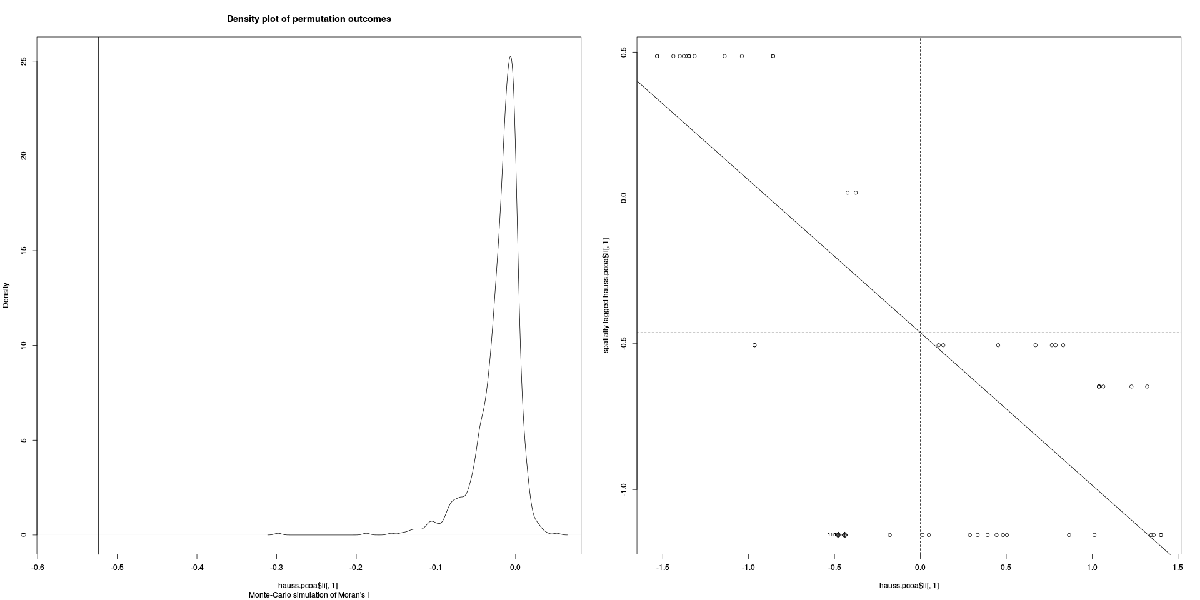
\includegraphics[width=\textwidth]{moran1.png}
\begin{footnotesize}
We tested hypothesis ``greater'' --- there is \textbf{no} significant positive autocorrelation
\end{footnotesize}
\end{frame}


\begin{frame}[fragile]{Calculation of Moran's \textit{I} (2$^{nd}$ axis)}
  \begin{spluscode}
    # Test of Moran's I for 2nd PCoA axis
    moran.test(x=hauss.pcoa$li[,2], listw=hauss.connectivity,
      alternative="greater", randomisation=TRUE)
    hauss.pcoa2.mctest <- moran.mc(x=hauss.pcoa$li[,2],
      listw=hauss.connectivity, alternative="greater", nsim=1000)
    hauss.pcoa2.mctest
    # Output
    Monte-Carlo simulation of Moran's I
    data:  hauss.pcoa$li[, 2] 
    weights: hauss.connectivity  
    number of simulations + 1: 1001 
    statistic = 0.0545, observed rank = 1001, p-value = 0.000999
    alternative hypothesis: greater
    # Plots
    plot(hauss.pcoa2.mctest)
    moran.plot(x=hauss.pcoa$[,2], listw=hauss.connectivity)
  \end{spluscode}
\end{frame}

\begin{frame}{Second axis is surprisingly significant}
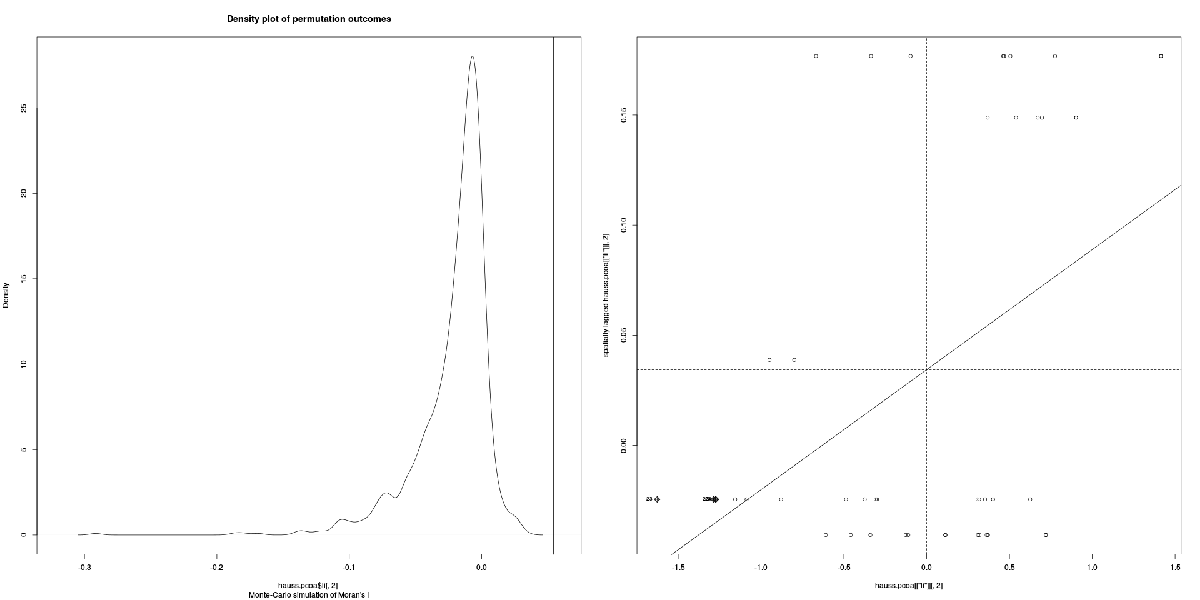
\includegraphics[width=\textwidth]{moran2.png}
\begin{footnotesize}
We tested hypothesis ``greater'' --- there \textbf{is} significant positive autocorrelation
\end{footnotesize}
\end{frame}

\subsection{sPCA}

\begin{frame}[fragile]{Spatial Analysis of Principal Components (sPCA)}
\begin{itemize}
 \item Implemented in adegenet, see \textbf{adegenetTutorial("spca")}
 \item Analyses matrix of relative allele frequencies of genotypes/populations and spatial weighting matrix
 \item The geographical matrix is usually (as for Moran's~\textit{I}) created by \textbf{chooseCN()} --- creates connectivity network among entities (genotypes/populations) --- spatial coordinates are not directly used
 \item When using \textbf{chooseCN()}, look at the documentation and try various methods with changing settings to see differences
\end{itemize}
  \begin{spluscode}
    data(rupica) # Loads adegenet's training dataset
    # Try various settings vor chooseCN (type=X) - type 1-4 as there
    # are identical coordinates (multiple sampling from same locality)
    chooseCN(xy=rupica$other$xy, ask=T, type=5/6/7, plot.nb=T, edit.nb=F)
    # See ?chooseCN for more details
  \end{spluscode}
\end{frame}

\begin{frame}[fragile]{Calculations of sPCA}
  \begin{spluscode}
    hauss.spca <- spca(obj=hauss.genind, cn=hauss.connectivity,
      scale=TRUE, scannf=TRUE)
    # Plot eigenvalues of sPCA - gobal vs. local structure
    barplot(height=hauss.spca$eig, main="Eigenvalues of sPCA",
      col=spectral(length(hauss.spca$eig)))
    legend("topright", fill=spectral(2), leg=c("Global structures",
      "Local structures")) # Add legend
    abline(h=0,col="grey") # Add line showing zero
    print.spca(hauss.spca) # Information about sPCA
    summary.spca(hauss.spca) # Summary of sPCA results
    # Shows connectivity network, 3 different scores
    # barplot of eigenvalues and eigenvalues decomposition
    plot.spca(hauss.spca)
    colorplot.spca(hauss.spca, cex=3) # Display of scores in color canals
    title("sPCA - colorplot of PC 1 and 2 (lagged scores)", line=1, cex=1.5)
    # Spatial and variance components of the eigenvalues
    screeplot.spca(x=hauss.spca, main=NULL)
  \end{spluscode}
\end{frame}

\begin{frame}{sPCA outputs}
\begin{center}
  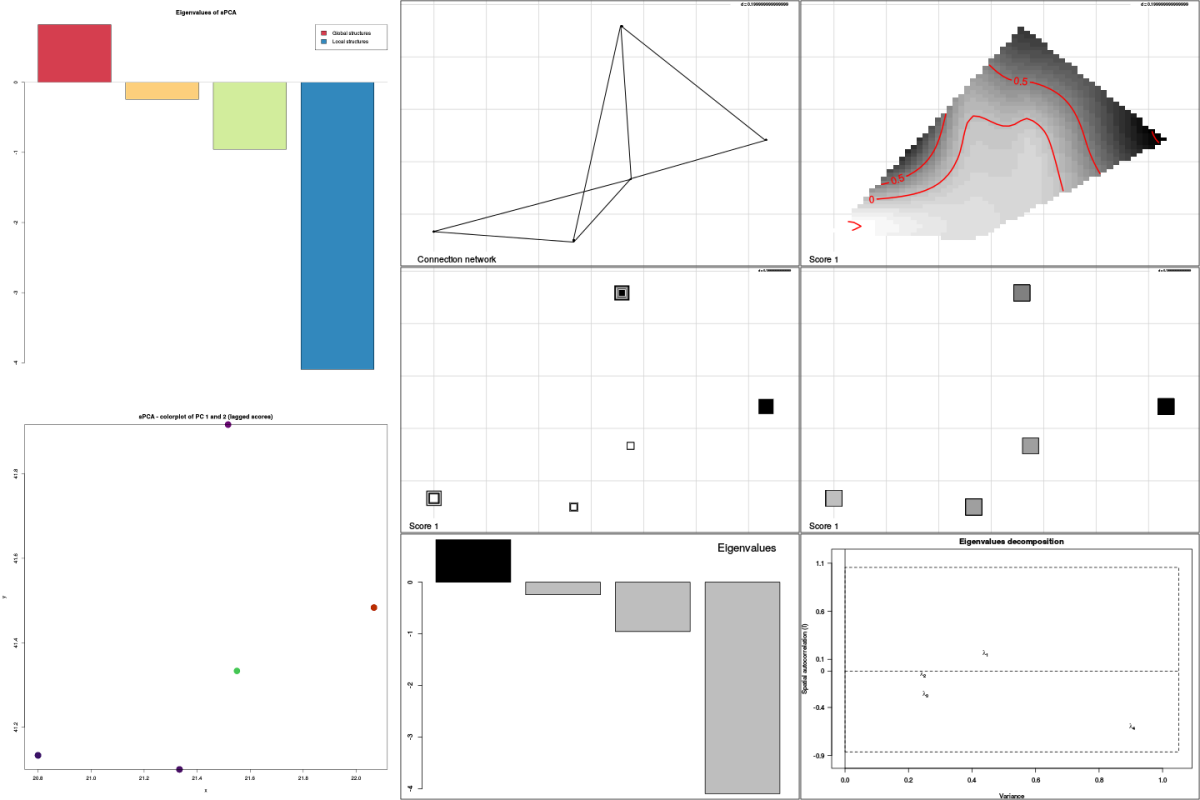
\includegraphics[width=\textwidth-1.5cm]{spca.png}
\end{center}
\end{frame}

\begin{frame}[fragile]{Map of genetic clines}
  \begin{spluscode}
    library(akima) # This library is needed for manipulation with coordinates
    hauss.spca.temp <- interp(other(hauss.genind)$xy[,1], other(
      hauss.genind)$xy[,2], hauss.spca$ls[,1], xo=seq(min(other(
      hauss.genind)$xy[,1]), max(other(hauss.genind)$xy[,1]), le=200), 
      yo=seq(min(other(hauss.genind)$xy[,2]), max(other(hauss.genind)$xy[,2]),
      le=200), duplicate="median")
    # For 1st axis
    image(x=hauss.spca.temp, col=spectral(100))
    s.value(dfxy=hauss.genind$other$xy, z=hauss.pcoa$li[,1], add.p=TRUE,
      csize=0.5, sub="PCoA - first PC", csub=2, possub="topleft")
    # For 2nd axis
    image(x=hauss.spca.temp, col=spectral(100))
    s.value(dfxy=hauss.genind$other$xy, z=hauss.pcoa[["li"]][,2], add.p=TRUE,
      csize=0.5, sub="PCoA - second PC", csub=2, possub="topleft")
  \end{spluscode}
\end{frame}

\begin{frame}[fragile]{sPCA outputs}
  \begin{spluscode}
    # Interpolated lagged score on a map
    hauss.spca.annot <- function() {
      title("sPCA - interpolated map of individual scores")
      points(other(hauss.genind)$xy[,1], other(hauss.genind)$xy[,2])
      }
    filled.contour(hauss.spca.temp, color.pal=colorRampPalette(
      lightseasun(100)), pch=20, nlevels=100, key.title=title("Lagged\n
      score 1"), plot.title=hauss.spca.annot())
  \end{spluscode}
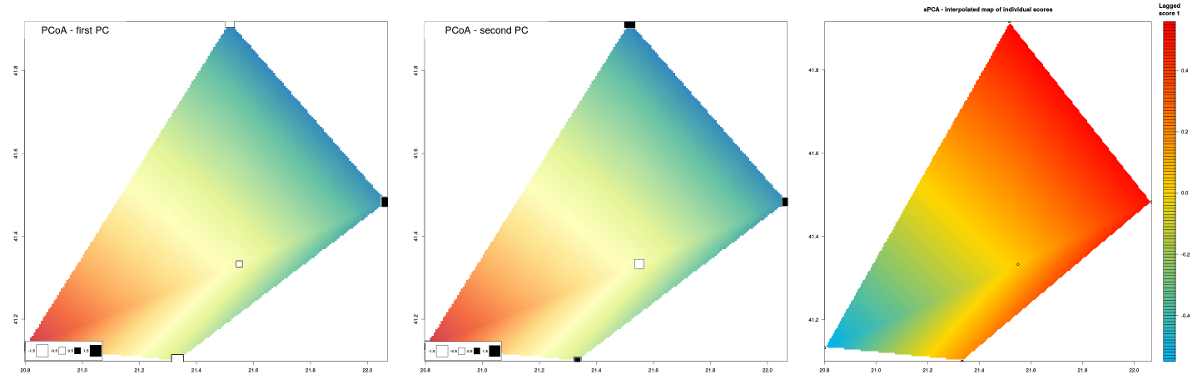
\includegraphics[width=\textwidth]{spca-pc.png}
\end{frame}

\begin{frame}[fragile]{Loading plots - which alleles contribute the most?}
  \begin{spluscode}
    hauss.spca.loadings <- hauss.spca[["c1"]][,1]^2
    names(hauss.spca.loadings) <- rownames(hauss.spca$c1)
    loadingplot(x=hauss.spca.loadings, xlab="Alleles", ylab="Weight of the
      alleles", main="Contribution of alleles to the first sPCA axis")
    boxplot(formula=hauss.spca.loadings~hauss.genind$loc.fac, las=3,
      ylab="Contribution", xlab="Marker", main="Contribution by markers
      into the first global score", col="grey")
  \end{spluscode}
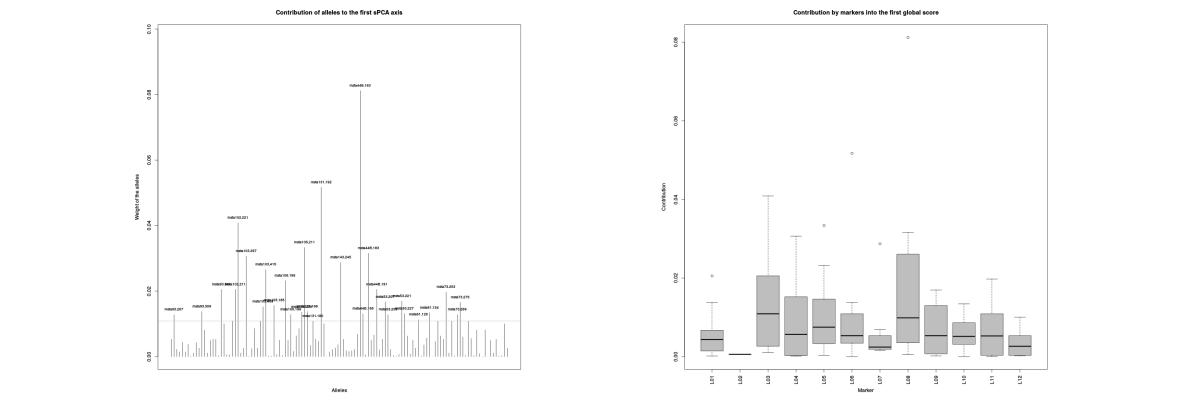
\includegraphics[width=\textwidth]{spca-loading.png}
\end{frame}

\subsection{Monmonier}

\begin{frame}[fragile]{Monmonier's algorithm --- genetic boundaries}
\begin{itemize}
 \item Finds boundaries of maximum differences between contiguous polygons of a tesselation
 \item Detects genetic boundaries among georeferecend genotypes (or populations)
 \item For more information see \textbf{adegenetTutorial("basics")}
 \item Requires every point to have unique coordinates (use \textbf{jitter()} when having same coordinates from one locality)
 \item Example here is on population level, which is not ideal for all cases
\end{itemize}
  \begin{spluscode}
    # Calculates Monmonier's function (for threshold use 'd')
    hauss.monmonier <- monmonier(xy=hauss.genpop$other$xy, dist=
      dist(hauss.genpop@tab), cn=chooseCN(hauss.genpop$other$xy,
      ask=FALSE, type=2, plot.nb=FALSE, edit.nb=FALSE), nrun=1)
    coords.monmonier(hauss.monmonier) # See result as text
  \end{spluscode}
\end{frame}

\begin{frame}[fragile]{Plot genetic boundaries}
\begin{multicols}{2}
  \begin{spluscode}
    plot.monmonier(hauss.monmonier,
      add.arrows=FALSE, bwd=10,
      sub="Monmonier plot", csub=2)
    points(hauss.genpop$other$xy,
      cex=2.5, pch=20, col="red")
    text(x=hauss.genpop$other$xy$lon,
      y=hauss.genpop$other$xy$lat,
      labels=hauss.genpop@pop.names,
      cex=3)
    legend("bottomright",
      leg="Genetic boundaries\n
      among populations")
    # See ?points, ?text and ?legend
  \end{spluscode}
  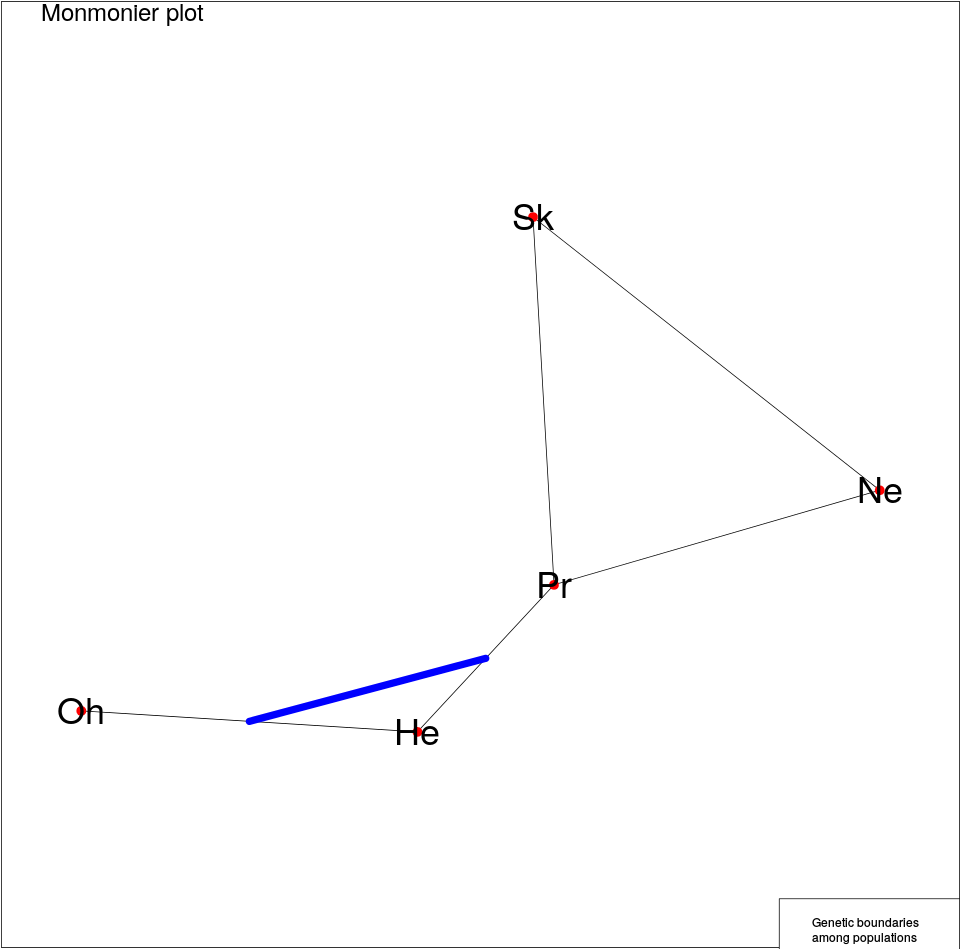
\includegraphics[height=6cm]{monmonier.png}
\end{multicols}
\end{frame}

\begin{frame}[fragile]{Monmonier notes}
\begin{itemize}
 \item Sometimes it is needed to get rid of random noise in data. To do so use as parameter \textbf{dist} of \textbf{monmonier()} table from PCA (\textbf{pcaObject\$li}):
\end{itemize}
  \begin{spluscode}
    monmonier(..., dist=dudi.pco(d=dist(x=GenindObject$tab),
      scannf=FALSE, nf=1)$li, ...)
  \end{spluscode}
\begin{itemize}
 \item Generally (when dataset is bigged and more diverse) it is recommended to run it several times (parameter \textbf{nrun}) --- there will be several iterations
 \item See \textbf{?plot.monmonier} for various graphical parameters to customize the plot
 \item Use \textbf{points()} to add for example coloured symbols of samples and/or \textbf{text()} to add text labels
\end{itemize}
\end{frame}

\subsection{Mantel test}

\begin{frame}[fragile]{Mantel test --- isolation by distance}
  \begin{spluscode}
    # Geographical distance
    hauss.gdist <- dist(x=hauss.genind$other$xy, method="euclidean",
      diag=TRUE, upper=TRUE)
    # Mantel test
    hauss.mantel <- mantel.randtest(m1=hauss.dist, m2=hauss.gdist,
      nrepet=1000)
    hauss.mantel # See text output
    plot(hauss.mantel, nclass=30)
    # Libraries required by mantel.correlog:
    library(permute)
    library(lattice)
    library(vegan)
    # Different implementation of Mantel test testing distance classes
    hauss.mantel.cor <- mantel.correlog(D.eco=hauss.dist,D.geo=hauss.gdist,
      XY=NULL, n.class=0, break.pts=NULL, cutoff=FALSE, r.type="pearson",
      nperm=1000, mult="holm", progressive=TRUE)
    # See results for respective classes
    hauss.mantel.cor
    summary(hauss.mantel.cor)
  \end{spluscode}
\end{frame}

\begin{frame}[fragile]{Mantel test outputs --- strongly significant}
\begin{multicols}{2}
  \begin{verbatim}
> hauss.mantel
Monte-Carlo test
Call: mantel.randtest(m1 =
  hauss.dist, m2 = 
  hauss.gdist, nrepet = 1000)
Observation: 0.35409
Based on 1000 replicates
Simulated p-value: 0.000999001
Alternative hypothesis: greater
   Std.Obs Expectation  Variance
7.61967545 0.001687140 0.0021389
  \end{verbatim}
  \begin{spluscode}
    # Plot correlogram (next slide)
    plot(hauss.mantel.cor)
  \end{spluscode}
  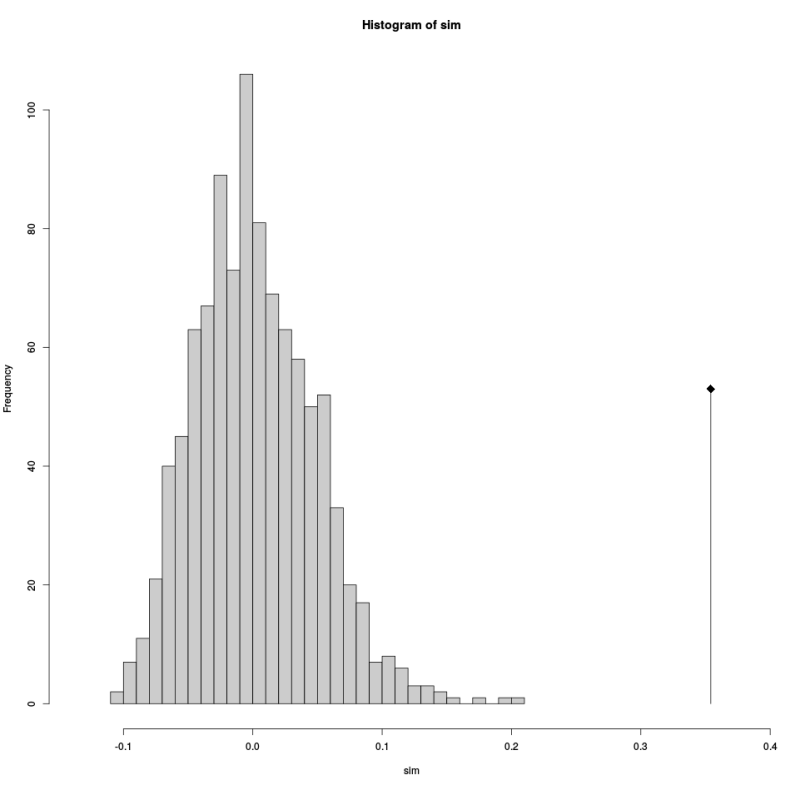
\includegraphics[height=6cm]{mantel.png}
\end{multicols}
\end{frame}

\begin{frame}{Plot of Mantel Correlogram Analysis}
  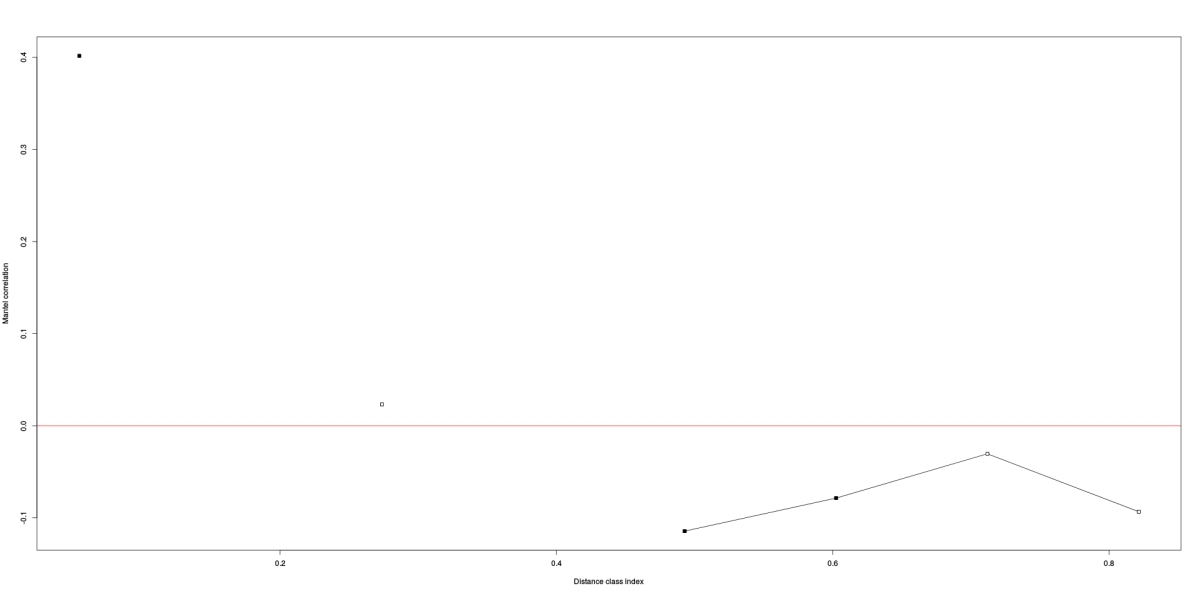
\includegraphics[width=\textwidth]{mantel-cor.png}
\end{frame}

\subsection{Geneland}

\begin{frame}[fragile]{About Geneland}
\begin{multicols}{2}
\begin{itemize}
 \item Works with haploid and diploid codominant markers (microsattelites or SNPs)
 \item Spatially explicit Bayesian clustering
 \item Produces maps of distribution of inferred genetic clusters
 \item Relative complicated tool with various modelling options
\end{itemize}
  \columnbreak
  \begin{spluscode}
    # Load needed libraries
    library(PBSmapping)
    library(RandomFields)
    library(fields)
    library(spam)
    library(grid)
    library(maps)
    library(tcltk)
    library(Geneland)
    # Graphical interface is available
    # we will use only command line
    Geneland.GUI()
  \end{spluscode}
\end{multicols}
For more information see \href{http://www2.imm.dtu.dk/~gigu/Geneland/}{http://www2.imm.dtu.dk/$\sim$gigu/Geneland/}
\end{frame}

\begin{frame}[fragile]{Loading and conversions of coordinates}
  \begin{spluscode}
    # Geneland requires specific coordinate space
    # hauss.cord is DF, we need just plain matrix
    hauss.geneland.coord <- as.matrix(hauss.coord)
    colnames(hauss.geneland.coord) <- c("X", "Y")
    attr(hauss.geneland.coord, "projection") <- "LL"
    attr(hauss.geneland.coord, "zone") <- NA
    hauss.geneland.coord.utm <- convUL(hauss.geneland.coord)
    dim(hauss.geneland.coord)
    hauss.geneland.coord
    dim(hauss.geneland.coord.utm)
    hauss.geneland.coord.utm # Final coordinates
    # Load data (only haploid or diploid data are supported)
    # only plain table with alleles
    hauss.geneland.data <- read.table(file=
      "http://trapa.cz/sites/default/rcourse/haussknechtii_geneland.txt",
      na.string="-999", header=FALSE, sep="\t")
    dim(hauss.geneland.data)
    hauss.geneland.data
  \end{spluscode}
\end{frame}

\begin{frame}[fragile]{Settings and running MCMC}
  \begin{spluscode}
    hauss.geneland.nrun <- 5 # Set number of independent runs
    hauss.geneland.burnin <- 100 # Set length of burnin chain
    hauss.geneland.maxpop <- 10 # Set maximal K (number of populations)
    # FOR loop will run several independent runs and produce output maps
    # of genetic clusters - outputs are written into subdirectory within
    # geneland directory (this has to exist prior launching analysis)
    for (hauss.geneland.irun in 1:hauss.geneland.nrun) {
      hauss.geneland.path.mcmc <- paste("geneland/", hauss.geneland.irun,
        "/", sep="") # paste is good especially for joining several texts
      # On Windows, remove following line and create subdirectories from
      # 1 to max K manually (creating subdirs in Windows is complicated)
      system(paste("mkdir ", hauss.geneland.path.mcmc)) # Creates subdirs
      # Inferrence - MCMC chain - see ?MCMC for details
      MCMC(coordinates=hauss.geneland.coord.utm, geno.dip.codom=
        hauss.geneland.data, path.mcmc=hauss.geneland.path.mcmc,
        delta.coord=0.001, varnpop=TRUE, npopmin=1, npopmax=
        hauss.geneland.maxpop, nit=10000, thinning=10,
        freq.model="Uncorrelated", spatial=TRUE)
      # For loop continues on next slide
  \end{spluscode}
\end{frame}

\begin{frame}[fragile]{Running MCMC}
  \begin{spluscode}
      # Start of FOR loop is on previous page
      # Post-process chains
      PostProcessChain(coordinates=hauss.geneland.coord.utm,
        path.mcmc=hauss.geneland.path.mcmc, nxdom=500, nydom=500,
        burnin=hauss.geneland.burnin)
      # Output
      # Simulated number of populations
      Plotnpop(path.mcmc=hauss.geneland.path.mcmc, printit=TRUE,
        file=paste(hauss.geneland.path.mcmc, "/geneland-number_of_clusters
        .pdf", sep=""), format="pdf", burnin=hauss.geneland.burnin)
      dev.off() # We must close graphical device manually
      # Map of estimated population membership
      PosteriorMode(coordinates=hauss.geneland.coord.utm, 
        path.mcmc=hauss.geneland.path.mcmc, printit=TRUE, format="pdf",
        file=paste(hauss.geneland.path.mcmc,"/geneland-map.pdf", sep=""))
      dev.off() # We must close graphical device manually
      } # End of FOR loop from previous slide
  \end{spluscode}
\end{frame}

\begin{frame}[fragile]{Estimate F$_{ST}$}
  \begin{spluscode}
    # Prepare list to record values of Fst for all runs
    hauss.geneland.fstat <- list()
    # Estimate Fst
    for (hauss.geneland.irun in 1:hauss.geneland.nrun) {
      hauss.geneland.path.mcmc <- paste("geneland/", hauss.geneland.irun,
        "/", sep="")
      # F-statistics - Fis and Fst
      hauss.geneland.fstat[[hauss.geneland.irun]] <- Fstat.output(
        coordinates=hauss.geneland.coord.utm, genotypes=hauss.geneland.data,
        burnin=hauss.geneland.burnin, ploidy=2,
        path.mcmc=hauss.geneland.path.mcmc)
      }
      # Print Fst output
      hauss.geneland.fstat
  \end{spluscode}
\end{frame}

\begin{frame}[fragile]{MCMC inference under the admixture model}
  \begin{spluscode}
    for (hauss.geneland.irun in 1:hauss.geneland.nrun) {
      hauss.geneland.path.mcmc <- paste("geneland/",
        hauss.geneland.irun, "/", sep="")
      hauss.geneland.path.mcmc.adm <- paste(hauss.geneland.path.mcmc,
        "admixture", "/", sep="")
      # On Windows, remove following line of code and create in each
      # result directory (from 1 to max K) new subdirectory "admixture"
      # (creating subdirs in Windows is complicated)
      system(paste("mkdir ", hauss.geneland.path.mcmc.adm))
      HZ(coordinates=hauss.geneland.coord.utm, geno.dip.codom=
        hauss.geneland.data, path.mcmc.noadm=hauss.geneland.path.mcmc,
        nit=10000, thinning=10, path.mcmc.adm=hauss.geneland.path.mcmc.adm)
      }
  \end{spluscode}
\vfil
Currently, there is no much use for admixture results, at lest not without extra work\ldots
\end{frame}

\begin{frame}[fragile]{Produce maps of respective inferred clusters}
  \begin{spluscode}
    for (hauss.geneland.irun in 1:hauss.geneland.nrun) {
      hauss.geneland.path.mcmc <- paste("geneland/",
        hauss.geneland.irun, "/", sep="")
      # Maps - tesselations
      PlotTessellation(coordinates=hauss.geneland.coord.utm,
        path.mcmc=hauss.geneland.path.mcmc, printit=TRUE,
        path=hauss.geneland.path.mcmc)
      for (hauss.geneland.irun.img in 1:hauss.geneland.maxpop) {
        dev.off() } # We must close graphical device manually
      }
  \end{spluscode}
\vfil
Maps are produced as PS (PostScript) files. Not every graphical software can handle them (try for example \href{http://www.gimp.org/}{GIMP}). There are as many plots as was maximal K, but only those up to inferred number of clusters have some content.
\end{frame}

\begin{frame}[fragile]{Determine which cluster is the best}
  \begin{spluscode}
    # Calculate average posterior probability
    hauss.geneland.lpd <- rep(NA, hauss.geneland.nrun)
    for (hauss.geneland.irun in 1:hauss.geneland.nrun) {
      hauss.geneland.path.mcmc <- paste("geneland/",
        hauss.geneland.irun, "/", sep="")
      hauss.geneland.path.lpd <- paste(hauss.geneland.path.mcmc,
        "log.posterior.density.txt", sep="")
      hauss.geneland.lpd[hauss.geneland.irun] <- 
        mean(scan(hauss.geneland.path.lpd)[-(1:hauss.geneland.burnin)])
      }
    # Sorts runs according to decreasing posterior probability
    # the first one is the best
    order(hauss.geneland.lpd, decreasing=TRUE)
    hauss.geneland.lpd
  \end{spluscode}
\vfil
We will use figures and F$_{ST}$ outputs only from the best run.
\end{frame}

\begin{frame}{MCMC chain, number of clusters and their map}
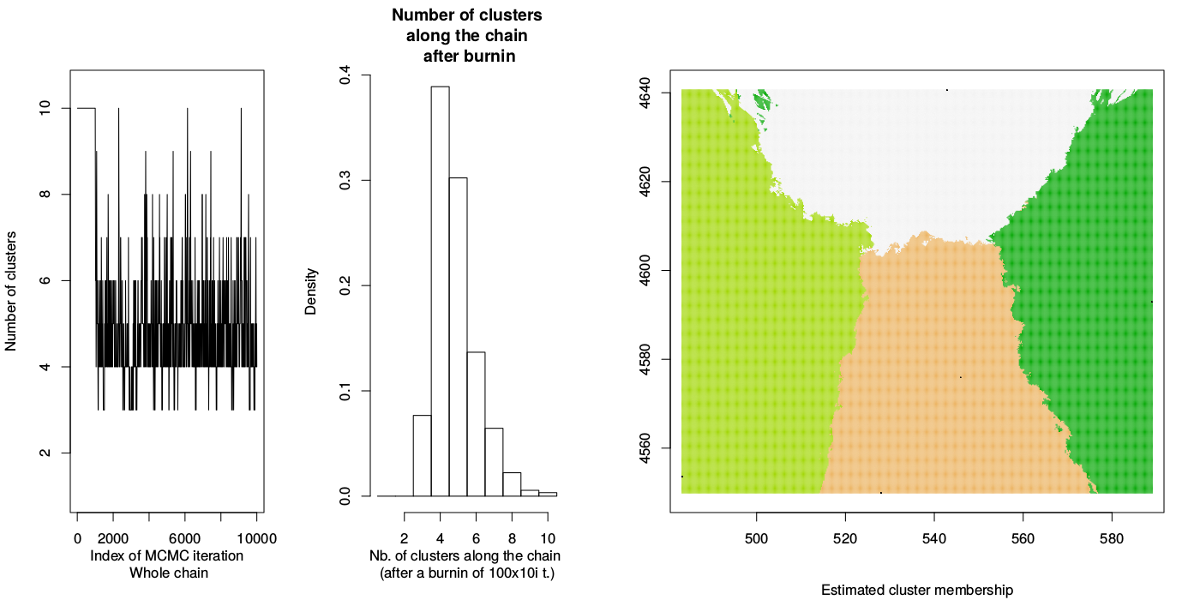
\includegraphics[width=\textwidth]{geneland1.png}
\end{frame}

\begin{frame}{Map of posterior probability of belonging into cluster 1}
\begin{center}
  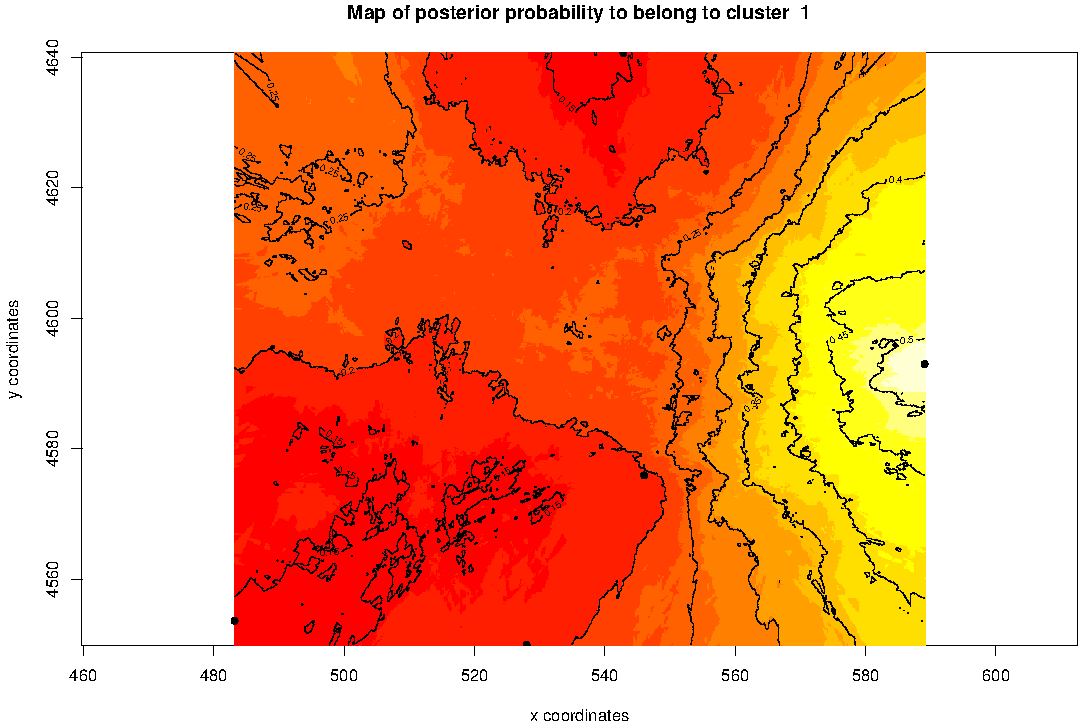
\includegraphics[width=\textwidth-1.5cm]{geneland2.png}
\end{center}
\end{frame}

\subsection{Plotting maps}

\begin{frame}[fragile]{Very basic mapping in R}
  \begin{spluscode}
    # Load libraries
    library(sp)
    library(rworldmap) # Basic world maps
    library(TeachingDemos) # To be able to move text little bit
    library(RgoogleMaps) # Google and OpenStreetMaps
    # Plot basic map with state boundaries within selected range
    plot(x=getMap(resolution="high"), xlim=c(19, 24), ylim=c(39, 44),
      asp=1, lwd=1.5)
    box() # Add frame around the map
    # Plot location points
    points(x=hauss.genpop@other$xy[["lon"]], y=hauss.genpop@other$xy
      [["lat"]], pch=15:19, col="red", cex=4)
    # Add text descriptions for points. Text is aside and with background
    shadowtext(x=hauss.genpop@other$xy[["lon"]], y=hauss.genpop@other$xy
      [["lat"]], labels=as.vector(hauss.genind@pop.names), col="black",
      bg="white", theta=seq(pi/4, 2*pi, length.out=8), r=0.15,
      pos=c(1, 3, 2, 4, 4), offset=0.75, cex=1.5)
  \end{spluscode}
\end{frame}

\begin{frame}[fragile]{Basic map and Google map}
\begin{multicols}{2}
  \begin{spluscode}
    # Insert legend
    legend(x="topright", inset=1/50,
      legend=c("He", "Oh", "Pr", "Ne",
      "Sk"), col="red", border="black",
      pch=15:19, pt.cex=2, bty="o",
      bg="lightgrey", box.lwd=1.5,
      cex=1.5, title="Populations")
    # Google map is produced into a
    # file. Parametr markers contain
    # data frame with coordinates and
    # possibly with another information
    hauss.gmap <- GetMap(center=c(lat=
      41, lon=21), size=c(640, 640),
      destfile="gmap.png", zoom=8,
      markers=hauss.coord,
      maptype="terrain")
  \end{spluscode}
  \begin{center}
    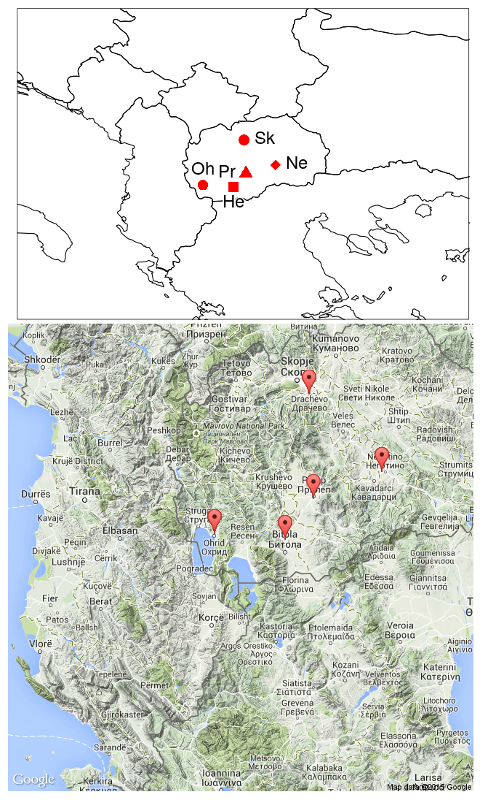
\includegraphics[height=6.5cm]{maps.png}
  \end{center}
\end{multicols}
\end{frame}

\begin{frame}[fragile]{OpenStreetMaps and datasets from mapproj}
  \begin{spluscode}
    # Plot on OpenStreeMap - server is commonly overloaded and doesn't
    # respond correctly - in fact, it rarely works...
    GetMap.OSM(lonR=c(18, 24), latR=c(39, 44), scale=200000, destfile=
      "osmmap.png", format="png", RETURNIMAGE=TRUE, GRAYSCALE=FALSE,
      NEWMAP=TRUE, verbose=1)
    # Plot on datasets from mapproj package
    library(maps) # Various maping tools (plotting, ...)
    library(mapdata) # More detailed maps, but political boundaries often
          # outdatet, see http://cran.r-project.org/web/packages/mapdata/
    library(mapproj) # Converts latitude/longitude into projected coordinates
    # Plot a map, check parameters
    # Check among others "projection" and ?mapproject for its details
    map(database="worldHires", boundary=TRUE, interior=TRUE, fill=TRUE,
      col="lightgrey", plot=TRUE, xlim=c(16, 27), ylim=c(37, 46))
    # If you'd use projection, use - mapproject to convert also coordinates!
    # See ?mapproject for details
    points(x=hauss.genpop@other$xy[["lon"]], y=hauss.genpop@other$xy
      [["lat"]], pch=15:19, col="red", cex=4)
  \end{spluscode}
\end{frame}

\begin{frame}[fragile]{Plotting on SHP files I}
\begin{scriptsize}
  Get SHP files from \href{http://trapa.cz/sites/default/rcourse/macedonia.zip}{http://trapa.cz/sites/default/rcourse/macedonia.zip}
\end{scriptsize}
  \begin{spluscode}
    library(maptools)
    # Load SHP file
    # Data from http://download.geofabrik.de/europe/macedonia.html
    # Directory has to contain also respective DBF and SHX files
    # (same name, only different extension)
    # There are several functions readShape* - select appropriate
    # according to data stored in respective SHP file
    macedonia_building <- readShapeLines(fn="macedonia_buildings.shp")
    plot(macedonia_building)
    macedonia_landuse <- readShapeLines(fn="macedonia_landuse.shp")
    plot(macedonia_landuse)
    macedonia_natural <- readShapeLines(fn="macedonia_natural.shp")
    plot(macedonia_natural)
    macedonia_railways <- readShapeLines(fn="macedonia_railways.shp")
    plot(macedonia_railways)
    macedonia_roads <- readShapeLines(fn="macedonia_roads.shp")
  \end{spluscode}
\end{frame}

\begin{frame}[fragile]{Plotting on SHP files II}
  \begin{spluscode}
    plot(macedonia_roads)
    macedonia_waterways <- readShapeLines(fn="macedonia_waterways.shp")
    plot(macedonia_waterways)
    # Plot all layers into single image
    plot(macedonia_building)
    plot(macedonia_landuse, add=TRUE, col="darkgreen", fill=TRUE)
    plot(macedonia_natural, add=TRUE, col="green", fill=TRUE)
    plot(macedonia_railways, add=TRUE, col="brown", lty="dotted")
    plot(macedonia_roads, add=TRUE, col="orange")
    plot(macedonia_waterways, add=TRUE, col="blue", lwd=2)
    # Add sampling points
    points(x=hauss.genpop@other$xy[["lon"]], y=hauss.genpop@other$
      xy[["lat"]], pch=15:19, col="red", cex=4)
    # Add description of psampling points
    shadowtext(x=hauss.genpop@other$xy[["lon"]], y=hauss.genpop@other$
      xy[["lat"]], labels=as.vector(hauss.genind@pop.names), col="black",
      bg="white", theta=seq(pi/4, 2*pi, length.out=8), r=0.15,
      pos=c(1, 3, 2, 4, 4), offset=0.75, cex=1.5)
  \end{spluscode}
\end{frame}

\begin{frame}[fragile]{Plotting on SHP files III}
  \begin{spluscode}
    # Add legend
    legend(x="topright", inset=1/50, legend=c("He", "Oh", "Pr", "Ne",
      "Sk"), col="red", border="black", pch=15:19, pt.cex=2, bty="o",
      bg="lightgrey", box.lwd=1.5, cex=1.5, title="Populations")
  \end{spluscode}
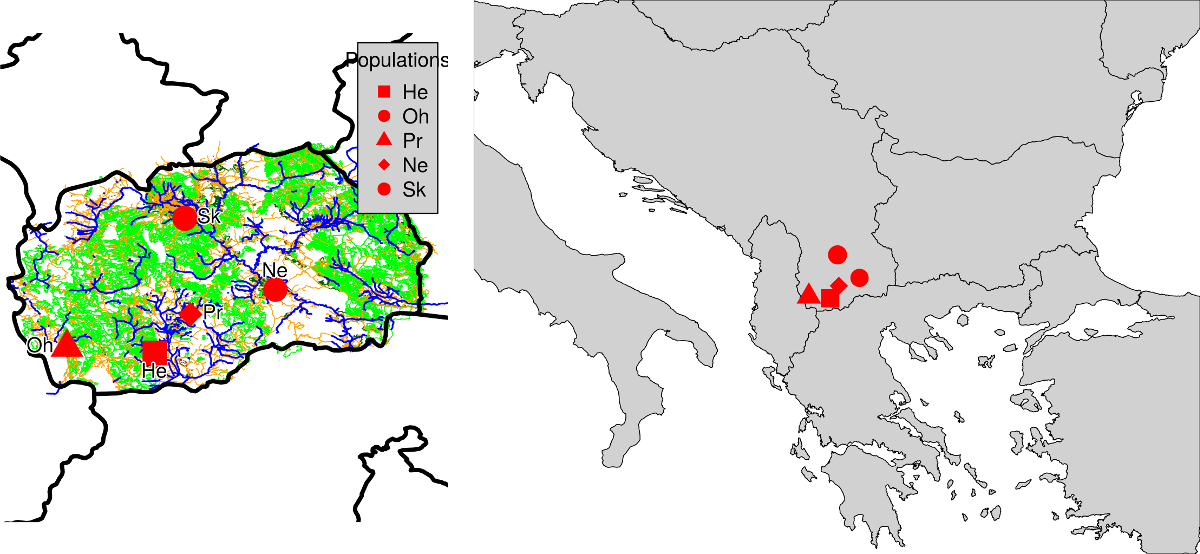
\includegraphics[width=\textwidth]{mapy.png}
\end{frame}

\section{Structure}

\begin{frame}[fragile]{Running Structure in parallel with R}
\begin{itemize}
 \item Population genetic software for Bayesian clustering \href{http://pritchardlab.stanford.edu/software.html}{Structure} requires several runs for each K and various Ks. It can result in hundreds runs
 \item With should use power of modern multi-core CPUs
 \item \href{https://r-forge.r-project.org/R/?group_id=1636}{ParallelStructure} library can optimally distribute computations of independent Structure runs among CPU cores
 \item When using it, cite \href{http://www.plosone.org/article/info\%3Adoi\%2F10.1371\%2Fjournal.pone.0070651}{Besnier \& Glover 2013}
 \item I show slightly modified way from \href{http://www.molecularecologist.com/2013/09/using-r-to-run-parallel-analyses-of-population-genetic-data-in-structure-parallelstructure/}{The Molecular Ecologist}
\end{itemize}
  \begin{spluscode}
    # Prepare special directory and set working directory
    setwd("~/dokumenty/fakulta/vyuka/r_mol_data/priklady/structure/")
    library(ParallelStructure) # Load the library
    # See Structure manual and function's documentation
    # It takes more or less same parameter as for normal Structure
    ?parallel_structure
    # Author's recommend to run it without GUI and not on Windows
  \end{spluscode}
\end{frame}

\begin{frame}{Preparing for ParallelStructure}
Within working ``structure'' directory you need
\begin{itemize}
 \item Subdirectory for results
 \item Text file describing jobs (``joblist'')
  \begin{itemize}
    \item One row for one Structure run
    \item Every line contains name of run, list of populations separated by comas (e.g. 1,2,3,4,5) --- you don't have to use all populations in all runs
    \item K for actual run
    \item Length of burnin chain
    \item Number of steps
    \item Columns are separated by spaces (or TABs)
  \end{itemize}
 \item Data input file
  \begin{itemize}
    \item Make it as simple as possible --- remove any unneeded columns
    \item For population names use subsequent number from 1 to number of populations
  \end{itemize}
\end{itemize}
\end{frame}

\begin{frame}[fragile]{Input files}
Joblist file:\\
\vfill
\begin{tabular}{lllll}
S02 & 1,2,3,4,5 & 1 & 500 & 10000\\
S06 & 1,2,3,4,5 & 2 & 500 & 10000\\
S08 & 1,2,3,4,5 & 2 & 500 & 10000\\
... & ... & ... & ... & ...\\
\end{tabular}
\vfill
Input file:\\
\vfill
\begin{tabular}{lllllllllll}
 & & & msta93 & msta101 & msta102 & msta103 & ...\\
H01 & 1 & 0 & 269 & 198 & 221 & 419 & ...\\
H01 & 1 & 0 & 269 & 198 & 223 & 419 & ...\\
H02 & 1 & 0 & 275 & 198 & 221 & 419 & ...\\
H02 & 1 & 0 & 283 & 198 & 223 & 419 & ...\\
... & ... & ... & ... & ... & ... & ... & ...
\end{tabular}
\end{frame}

\begin{frame}[fragile]{Running ParallelStructure}
  \begin{spluscode}
    parallel_structure(joblist="joblist.txt", n_cpu=7, structure_path=
      "~/bin/", infile="hauss_stru.in", outpath="results/", numinds=47,
      numloci=12, plot_output=1, label=1, popdata=1, popflag=1,
      phenotypes=0, markernames=1, mapdist=0, onerowperind=0, phaseinfo=0,
      extracol=0, missing=-9, ploidy=2, usepopinfo=0, revert_convert=1,
      printqhat=1, locdata=0, recessivealleles=0, phased=0, noadmix=0,
      linkage=0, locprior=0, inferalpha=1)
  \end{spluscode}
\begin{itemize}
 \item Choose \textbf{n\_cpu} according to your computer
 \item \textbf{structure\_path} points to \alert{directory} containing Structure binary
 \item \textbf{outpath} should aim to empty directory
 \item \textbf{plot\_output=1} will produce plots for all runs
 \item Check all other settings according to Structure manual and your needs
 \item Get input file \href{https://trapa.cz/sites/default/rcourse/hauss_stru.in}{https://trapa.cz/sites/default/rcourse/hauss\_stru.in} and joblist \href{https://trapa.cz/sites/default/rcourse/joblist.txt}{https://trapa.cz/sites/default/rcourse/joblist.txt}
\end{itemize}
\end{frame}

\begin{frame}[fragile]{ParallelStructure and Windows}
\begin{itemize}
 \item Authors do not recommend to run ParallelStructure on Windows\ldots
 \item \textbf{parallel\_structure()} is missing paralleling library which is not available on Windows, instead try
\end{itemize}
  \begin{spluscode}
    # Install Rmpi library required by ParallelStructure for
    # parallelisation on Windows
    install.packages("Rmpi")
    library(Rmpi)
    # Instead of parallel_structure() use MPI_structure()
    # with same arguments
    MPI_structure(...) # Same arguments as on previous slide
  \end{spluscode}
\begin{itemize}
 \item If this fails, look for some UNIX machine (Linux, Mac OS X, BSD,~\ldots)\ldots
\end{itemize}
\end{frame}

\subsection{Postprocessing}

\begin{frame}[fragile]{Postprocess Structure results --- select the best K}
 \begin{itemize}
  \item Using Structure-sum-2009 R script by \href{http://en.uit.no/om/enhet/ansatte/person?p_document_id=41186&p_dimension_id=88165}{Dorothee Ehrich}
 \end{itemize}
 \begin{spluscode}
    # Load the script
    source("structure-sum-2009.r")
    # Create new directory with result files results_job_*_f and set
    # working directory accordingly
    setwd("/home/vojta/dokumenty/fakulta/vyuka/r_mol_data/priklady/
      structure/structure_sum/")
  \end{spluscode}
 \begin{itemize}
  \item When using it, cite \href{http://onlinelibrary.wiley.com/doi/10.1111/j.1471-8286.2006.01380.x/abstract}{Ehrich 2006}. If you don't have the script, ask (it is not my so I don't want to post it on the net)
  \item Prepare list\_k.txt containing on each line K and name of output file
  \item Get list K from \href{https://trapa.cz/sites/default/rcourse/list_k.txt}{https://trapa.cz/sites/default/rcourse/list\_k.txt}
  \item Joblist look like this:
 \end{itemize}
\begin{verbatim}
2    results_job_S010_f
3    results_job_S011_f
...  ...
\end{verbatim}
\end{frame}

\begin{frame}[fragile]{Run Structure-sum}
  \begin{spluscode}
    # See documentation for details. Functions take as an argument
    # list_k file and number of populations
    Structure.table("list_k.txt", 5)
    Structure.simil("list_k.txt", 5)
    Structure.deltaK("list_k.txt", 5)
    graphics.off() # Close graphics
    Structure.cluster("list_k.txt", 5)
    # Reordering ("alignment") of runs to get same clusters in same
    # columns (prepare respective list_k files - one for each K)
    Structure.order("list_k_02.txt", 5)
    Structure.order("list_k_03.txt", 5)
    Structure.order("list_k_04.txt", 5)
    Structure.order("list_k_05.txt", 5)
    Structure.order("list_k_06.txt", 5)
    Structure.order("list_k_07.txt", 5)
    # Continue with CLUMPP and distruct...
  \end{spluscode}
Details: \href{https://trapa.cz/en/structure-r-linux}{https://trapa.cz/en/structure-r-linux}
\end{frame}

\begin{frame}{Outputs of Structure-sum --- the best K is 2, may be 3 --- stability of runs, good posterior probability}{Results from different data set, not from our toy}
  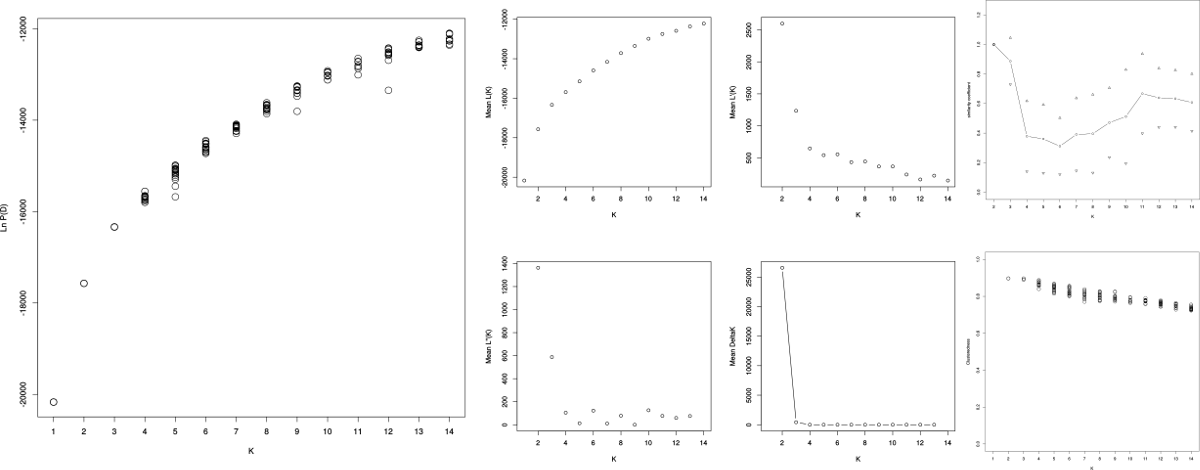
\includegraphics[width=\textwidth]{structure.png}
\end{frame}

\section{Alignment}

\subsection{MUSCLE}

\begin{frame}[fragile]{Multiple sequence alignment --- package muscle}
  \begin{spluscode}
    # Muscle has its own functions read.fasta and write.fasta
    library(muscle)
    # Reads local file and writes R object or external file
    # with alignment, you can use any command line argument
    # available for muscle, see ?muscle and its manual
    # Write result to external file
    muscle(seqs="usflu.fasta", out="usflu.aln", quiet=FALSE)
    # Write result to R object
    usflu.muscle <- muscle(seqs="usflu.fasta", out=NULL, quiet=FALSE)
    # Prints the alignment
    print(usflu.muscle, from=1, to=usflu.muscle[["length"]])
    class(usflu.muscle)
  \end{spluscode}
\begin{itemize}
 \item Package \href{http://cran.r-project.org/web/packages/muscle/index.html}{\textbf{muscle}} contains MUSCLE binary
 \item Read \href{http://www.drive5.com/muscle/manual/}{MUSCLE documentation} to get correct parameters (if you are not fine with defaults)
\end{itemize}
\end{frame}

\subsection{MAFFT}

\begin{frame}[fragile]{Multiple sequence alignment}
\begin{itemize}
 \item MUSCLE is available in package \textbf{muscle} (above) and in package \textbf{ape} --- first one reads FASTA files and writes external FASTA files or R objects of class ``muscle''. The latter reads and writes object of class ``DNAbin''
 \item ape also contains functions to use Clustal and T-Coffee --- both read and write DNAbin
 \item MAFFT is available from (same author) in packages \href{http://cran.r-project.org/web/packages/ips/index.html}{\textbf{ips}} and \href{http://www.christophheibl.de/Rpackages.html}{\textbf{phyloch}} --- both read and write DNAbin
\end{itemize}
  \begin{spluscode}
    library(colorspace) # Libraries needed by phyloch/ips
    library(XML)
    library(phyloch) # Alignment with mafft, you can also try package ips
    # Requires mafft binary on specific location
    # you might be needed to copy it or make symlink or so
    # read ?mafft and mafft's documentation
    meles.mafft <- mafft(x=meles.dna, method="localpair", maxiterate=100)
    meles.mafft
  \end{spluscode}
\end{frame}

\subsection{Clustal, MUSCLE and T-Coffee from ape}

\begin{frame}[fragile]{Clustal, MUSCLE and T-Coffee from ape}
  \begin{spluscode}
    class(meles.mafft)
    # read ?clustal and documentation of Clustal, Muscle and T-Coffee
    # when using them to set correct parameters
    clustal(x=meles.dna, pw.gapopen=10, pw.gapext=0.1, gapopen=10,
      gapext=0.2, quiet=FALSE, original.ordering=TRUE)
    meles.muscle <- muscle(x=meles.dna, exec="muscle",
      quiet=FALSE, original.ordering=TRUE)
    meles.muscle
    class(meles.muscle)
    # Plot the alignment - you can select which bases to plot
    # and/or modify colours
    image(x=meles.muscle, c("a", "t", "c" ,"g", "n"), col=rainbow(5))
    # Add grey dotted grid
    grid(nx=ncol(meles.muscle), ny=nrow(meles.muscle), col="lightgrey")
    # Remove gaps from alignment - destroy it
    meles.nogaps <- del.gaps(meles.muscle)
  \end{spluscode}
\end{frame}

\begin{frame}{Multiple sequence alignment with MUSCLE}
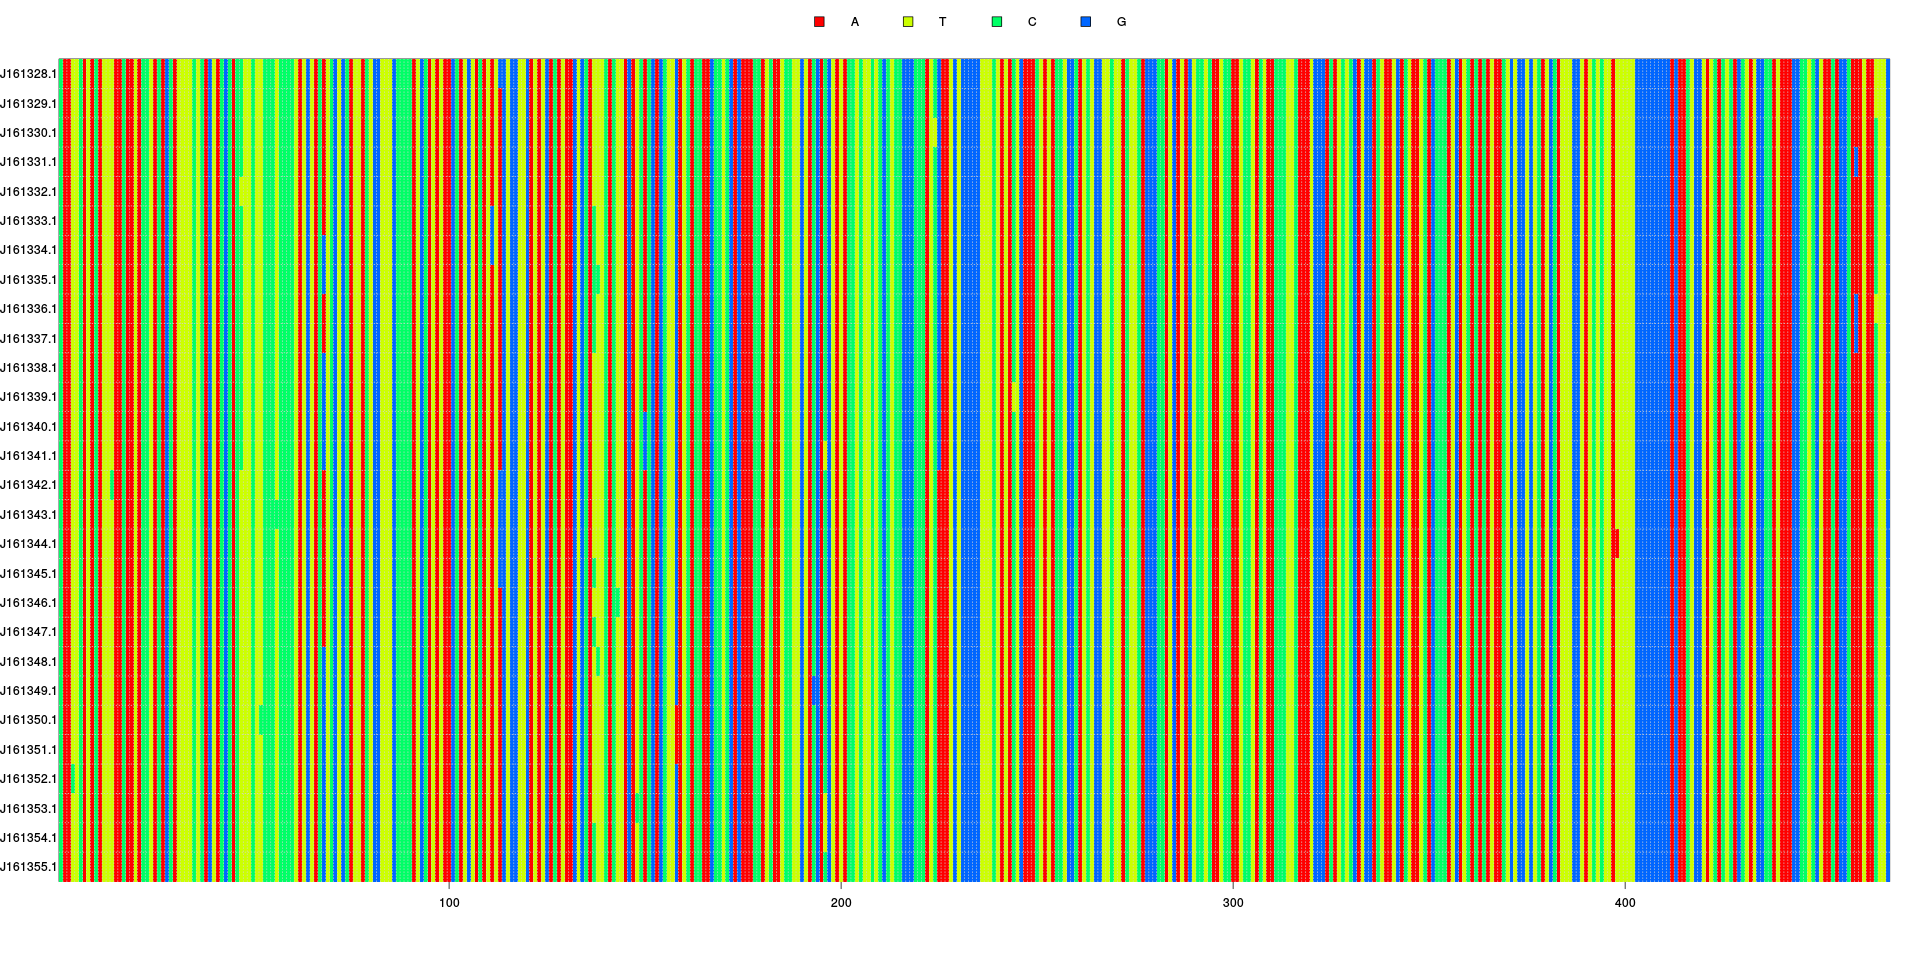
\includegraphics[width=\textwidth]{muscle.png}
\end{frame}

\section{Trees}

\subsection{Tree manipulations}

\begin{frame}[fragile]{Read and write tree and drop tips}
  \begin{spluscode}
    # Read trees in NEWICK format - single or multiple tree(s)
    oxalis.trees <- read.tree
      ("http://trapa.cz/sites/default/rcourse/oxalis.nwk")
    summary(oxalis.trees)
    length(oxalis.trees)
    names(oxalis.trees)
    # Export trees in NEWICK format
    write.tree(phy=oxalis.trees, file="trees.nwk")
    # Drop a tip from multiPhylo
    plot.multiPhylo(x=oxalis.trees)
    oxalis.trees.drop <- lapply(X=oxalis.trees, FUN=drop.tip, "TaxaOut")
    class(oxalis.trees.drop) <- "multiPhylo"
    plot.multiPhylo(x=oxalis.trees.drop)
    # Drop a tip from single tree
    plot.phylo(hauss.nj)
    hauss.nj.drop <- drop.tip(phy=hauss.nj, tip=47)
    plot.phylo(hauss.nj.drop)
  \end{spluscode}
\end{frame}

\begin{frame}[fragile]{Extract clades from trees and drop extinct tips}
  \begin{spluscode}
    # Interactively extract tree
    # Plot source tree
    plot.phylo(hauss.nj)
    # Select clade to extract by clicking on it
    hauss.nj.extracted <- extract.clade(phy=hauss.nj, interactive=TRUE)
    # See new extracted tree
    plot.phylo(hauss.nj.extracted)
    # Non-interactively extract tree
    hauss.nj.extracted <- extract.clade(phy=hauss.nj, node=60,
      interactive=FALSE)
    # See new extracted tree
    plot.phylo(hauss.nj.extracted)
    # Drop "extinct" tips - those who don't reach end the tree
    # tolerance is respective to the used metrics
    plot.phylo(hauss.nj)
    axisPhylo()
    hauss.nj.fossil <- drop.fossil(phy=hauss.nj, tol=0.25)
    plot.phylo(hauss.nj.fossil)
  \end{spluscode}
\end{frame}

\begin{frame}[fragile]{Join two trees, rotate tree}
  \begin{spluscode}
    # Bind two trees into one
    hauss.nj.bind <- bind.tree(x=hauss.nj.fossil, y=hauss.nj.extracted,
      where="root", position=0, interactive=FALSE)
    plot.phylo(hauss.nj.bind)
    # Bind two trees interactively
    # Plot tree receiving the new one
    plot.phylo(hauss.nj.fossil)
    # Select where to bind new tree to
    hauss.nj.bind <- bind.tree(x=hauss.nj.fossil, y=hauss.nj.extracted,
      interactive=TRUE)
    plot.phylo(hauss.nj.bind)
    # Rotate tree
    plot.phylo(hauss.nj)
    hauss.nj.rotated <- rotate(phy=hauss.nj, node="70")
    plot.phylo(hauss.nj.rotated)
  \end{spluscode}
\end{frame}

\begin{frame}[fragile]{Ladderize and (un)root the tree}
  \begin{spluscode}
    # Ladderize the tree
    plot.phylo(hauss.nj)
    hauss.nj.ladderized <- ladderize(hauss.nj)
    plot.phylo(hauss.nj.ladderized)
    # Root the tree
    plot.phylo(hauss.nj)
    print.phylo(hauss.nj)
    hauss.nj.rooted <- root(phy=hauss.nj, outgroup="10")
    print.phylo(hauss.nj.rooted)
    plot.phylo(hauss.nj.rooted)
    # Root the tree interactive
    plot.phylo(hauss.nj)
    hauss.nj.rooted <- root(phy=hauss.nj, interactive=TRUE)
    plot.phylo(hauss.nj.rooted)
    # unroot the tree
    unroot()
    # Check if it is rooted
    is.rooted()
  \end{spluscode}
\end{frame}

\begin{frame}[fragile]{Check tree and compute branch lengths and times}
  \begin{spluscode}
    # Check if the tree is ultrametric - is variance of distances
    # of all tips to node 0? It is required for some analysis
    is.ultrametric()
    # Make tree ultrametric
    chronos()
    ?chronos # Check it for mode how to calculate the lengths
    # chronos has more uses - it is mainly used for dating
    # Compute branch lengths for trees withou branch lengths
    ?compute.brlen # Check it for mode how to calculate the lengths
    compute.brlen()
    # Computes the branch lengths of a tree giving its branching
    # times (aka node ages or heights)
    compute.brtime()
    ?compute.brtima # Check it for mode how to calculate the lengths
  \end{spluscode}
Class ``multiPhylo'' is just a list of ``phylo'' objects to store multiple trees --- you can perform most of analysis on it as on phylo, commonly using \textbf{lapply} function (afterwards use class(x) <- "multiPhylo" to ensure other functions will see it as multiPhylo object).
\end{frame}

\subsection{Seeing trees in the forest}

\begin{frame}[fragile]{Topographical distances among trees I}
We have plenty of trees. How much are their topologies different?
  \begin{spluscode}
    library(gplots)
    library(corrplot)
    library(phytools)
    # Prepare matrix for distances
    oxalis.trees.d <- matrix(nrow=length(oxalis.trees),
      ncol=length(oxalis.trees))
    # Calculate pairwise topographic distances
    for (i in 1:length(oxalis.trees)) {
      for (j in i:length(oxalis.trees)) {
        print(c(i,j))
        oxalis.trees.d[i,j] <- dist.topo(oxalis.trees[[i]],
          oxalis.trees[[j]])
      }
    }
    # Basic information about the distance matrix
    dim(oxalis.trees.d)
    head.matrix(oxalis.trees.d)
  \end{spluscode}
\end{frame}

\begin{frame}[fragile]{Topographical distances among trees II}
Postprocess the matrix and plot it. There are several methods for calculating distance matrices among the trees --- some take branch lengths into account, some only topology.
  \begin{spluscode}
    # Add names of columns and rows
    colnames(oxalis.trees.d) <- names(oxalis.trees)
    rownames(oxalis.trees.d) <- names(oxalis.trees)
    # Make matrix symetric
    oxalis.trees.d[lower.tri(oxalis.trees.d)]=
      t(oxalis.trees.d)[lower.tri(oxalis.trees.d)]
    # Create heatmaps using heatmap.2 function from gplots package
    heatmap.2(x=oxalis.trees.d, Rowv=FALSE, Colv="Rowv", dendrogram="none",
      symm=TRUE, scale="none", na.rm=TRUE, revC=FALSE, col=rainbow(15),
      cellnote=oxalis.trees.d, notecex=1, notecol="white", trace="row",
      linecol="black", labRow=names(oxalis.trees),
      labCol=names(oxalis.trees), key=TRUE, keysize=2,
      density.info="density", symkey=FALSE, main="Correlation matrix of
      topographical distances", xlab=names(oxalis.trees),
      ylab=names(oxalis.trees))
  \end{spluscode}
\end{frame}

\begin{frame}[fragile]{Topographical distances among trees III}
Calculate Robinsons-Foulds distance (allow compare trees created by different algorithms) matrix among trees and plot it.
  \begin{spluscode}
    # Robinsons-Foulds distance
    oxalis.trees.d.rf <- multiRF(oxalis.trees)
    # Add names of columns and rows
    colnames(oxalis.trees.d.rf) <- names(oxalis.trees)
    rownames(oxalis.trees.d.rf) <- names(oxalis.trees)
    # Create heatmap using corrplot function from corrplot package
    corrplot(corr=oxalis.trees.d.rf, method="circle", type="upper",
      col=rainbow(15), title="Correlation matrix of topographical
      distances", is.corr=FALSE, diag=FALSE, outline=TRUE,
      order="alphabet", tl.pos="lt", tl.col="black")
    corrplot(corr=oxalis.trees.d.rf, method="number", type="lower",
      add=TRUE, col=rainbow(15), title="Correlation matrix of
      topographical distances", is.corr=FALSE, diag=FALSE,
      outline=FALSE, order="alphabet", tl.pos="ld", cl.pos="n")
  \end{spluscode}
\end{frame}

\begin{frame}{Topographical distances among trees IV --- the matrices}
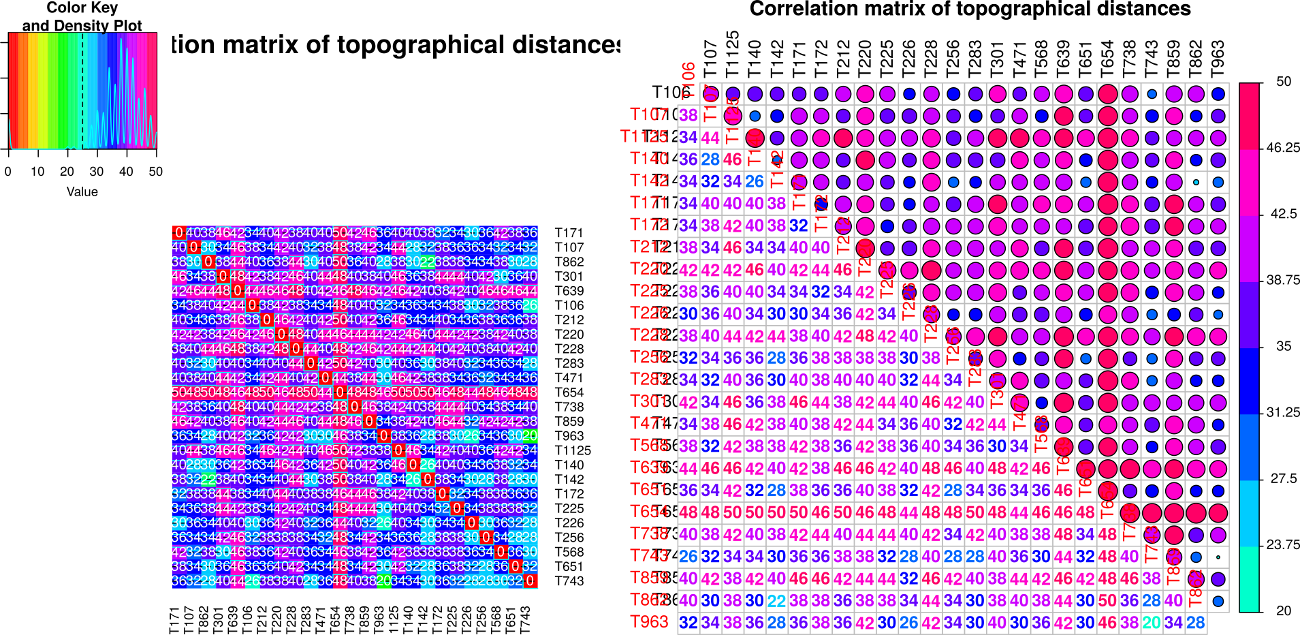
\includegraphics[width=\textwidth]{oxalis-dist.png}
\end{frame}

\begin{frame}[fragile]{Consensus tree}
\begin{multicols}{2}
  \begin{spluscode}
    # Root all trees
    oxalis.trees.rooted <- lapply
      (X=oxalis.trees, FUN=root,
      "TaxaOut")
    class(oxalis.trees.rooted) <-
      "multiPhylo"
    # Consenus tree (50 \% rule)
    oxalis.tree.con <- consensus
      (oxalis.trees.rooted, p=0.5,
      check.labels=TRUE)
    print.phylo(oxalis.tree.con)
    # Plot the tree
    plot.phylo(oxalis.tree.con,
      edge.width=2, label.offset=0.3)
    axisPhylo(side=1)
    # What a nice tree... :-P
  \end{spluscode}
  \columnbreak
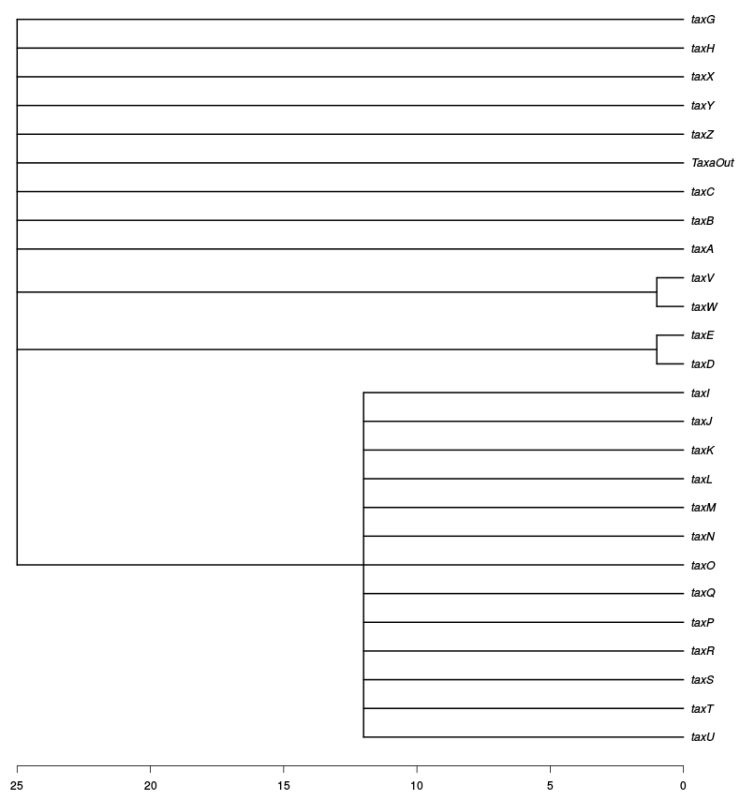
\includegraphics[height=6.5cm]{oxalis-cons.png}
\end{multicols}
\end{frame}

\begin{frame}[fragile]{Species tree --- all trees must be ultrametric}
\begin{multicols}{2}
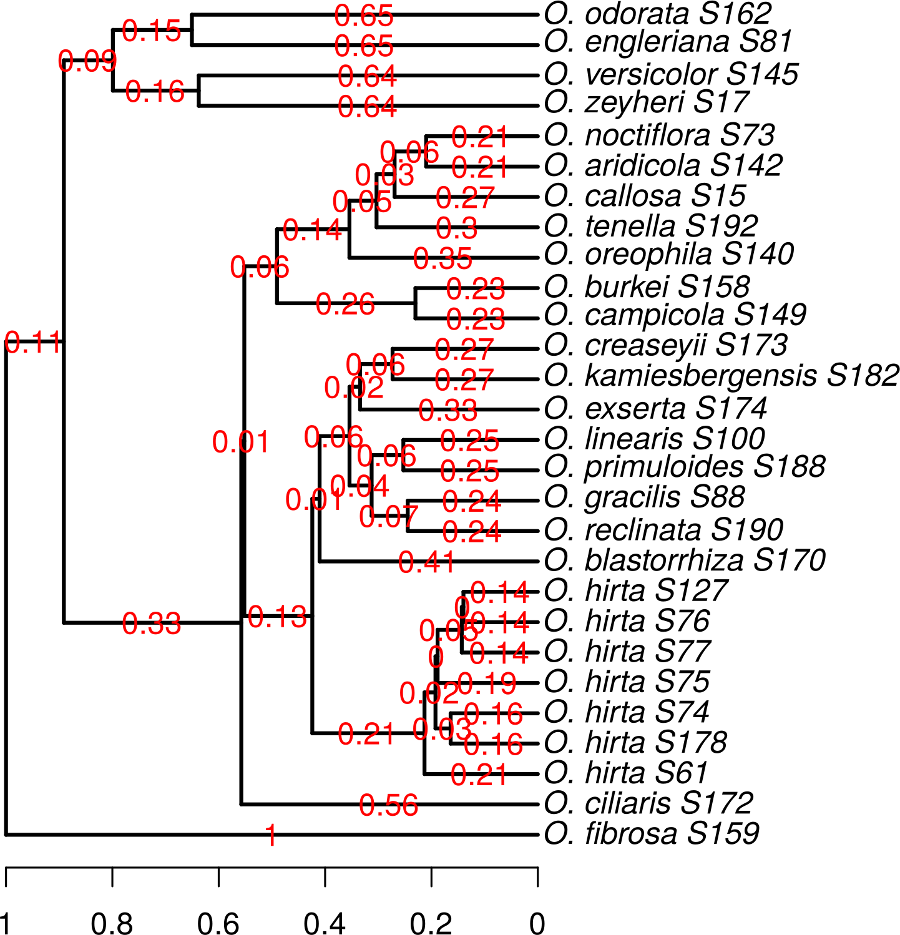
\includegraphics[height=6.5cm]{oxalis-sp.png}
  \columnbreak
  \begin{spluscode}
    # Chronos scale trees
    oxalis.trees.ultra <- lapply
      (X=oxalis.trees.rooted,
      FUN=chronos, model="correlated")
    class(oxalis.trees.ultra) <-
      "multiPhylo"
    # Mean distances
    oxalis.tree.sp.mean <- speciesTree
      (oxalis.trees.ultra, mean)
    # Plot the tree
    plot.phylo(oxalis.tree.sp.mean,
      edge.width=2, label.offset=0.01)
    edgelabels(text=round(oxalis.
      tree.sp.mean[["edge.length"]],
      digits=2), frame="none",
      col="red", bg="none")
    axisPhylo(side=1)
  \end{spluscode}
\end{multicols}
\end{frame}

\begin{frame}[fragile]{Parsimony super tree}
\begin{multicols}{2}
  \begin{spluscode}
    library(phangorn)
    oxalis.tree.sp <- superTree(tree=
      oxalis.trees.rooted, method=
      "optim.parsimony", rooted=TRUE)
    print.phylo(oxalis.tree.sp)
    plot.phylo(oxalis.tree.sp,
      edge.width=2, label.offset=0.01)
    axisPhylo(side=1)
  \end{spluscode}
  Currently, there is no package for coalescence based approach for creation of species tree from multiple gene trees. This function was in package \href{https://code.google.com/p/phybase/}{phybase}, but it is abandoned and doesn't install in R~3 without hacks
  \columnbreak
  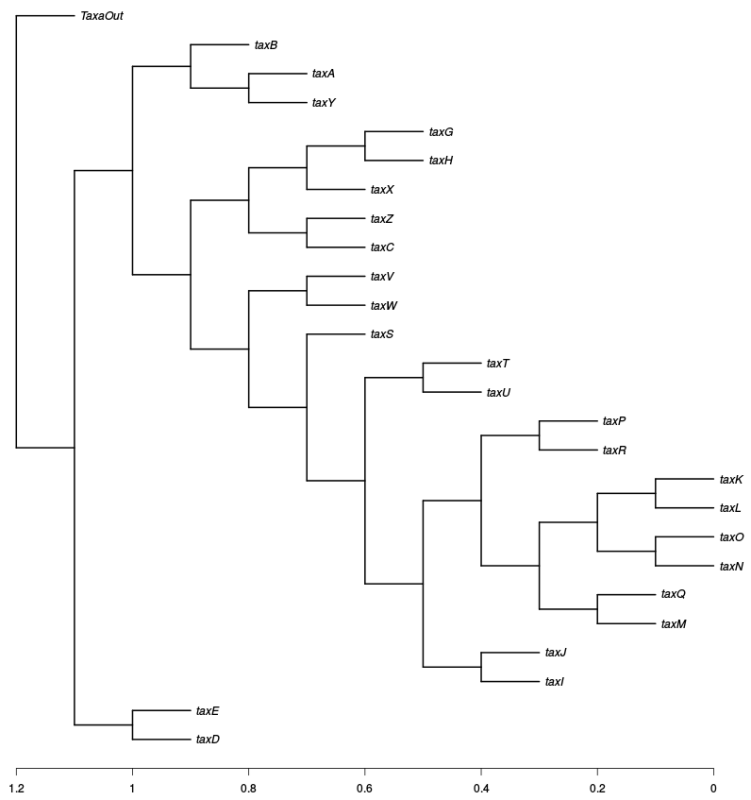
\includegraphics[height=6.5cm]{oxalis-pars.png}
\end{multicols}
\end{frame}

\begin{frame}[fragile]{Density tree}
  \begin{spluscode}
    densiTree(x=oxalis.trees.ultra, type="cladogram", alpha=0.5,
      consensus=oxalis.tree.sp.mean, scaleX=TRUE, col=c("black",
      "green", "blue", "red"), cex=1.5)
  \end{spluscode}
\begin{center}
  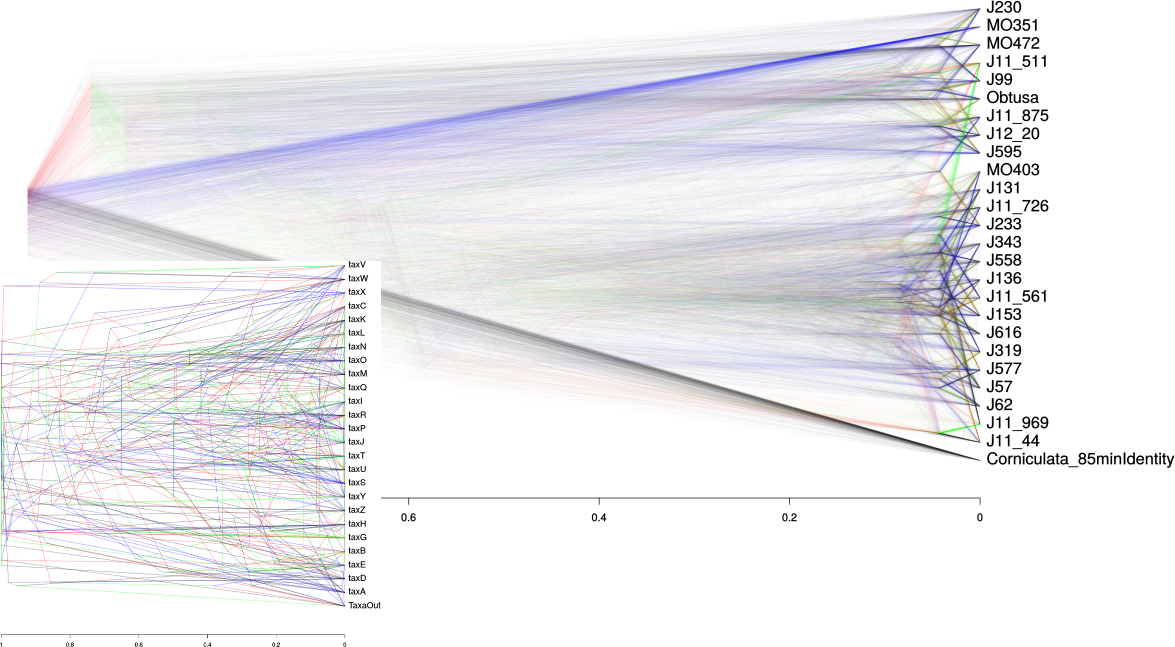
\includegraphics[width=\textwidth-1.5cm]{oxalis_density_good.png}
\end{center}
\end{frame}

\begin{frame}[fragile]{Networks}
\begin{multicols}{2}
  \begin{spluscode}
    oxalis.tree.net <- consensusNet
      (oxalis.trees.rooted, prob=0.25)
  \end{spluscode}
  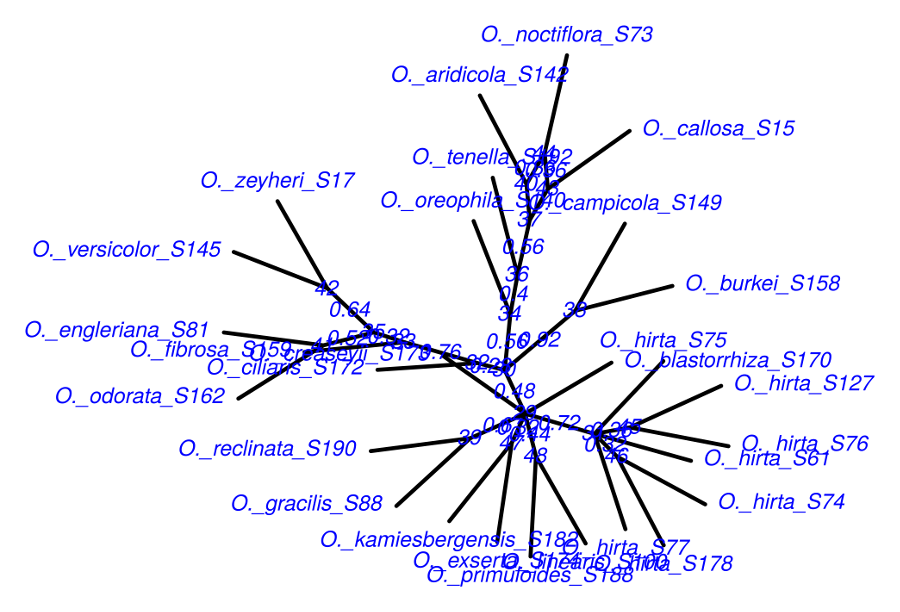
\includegraphics[height=5.5cm]{oxalis-net.png}
  \columnbreak
  \begin{spluscode}
    plot.networx(x=oxalis.tree.net,
      planar=FALSE, type="2D",
      use.edge.length=TRUE,
      show.tip.label=TRUE,
      show.edge.label=TRUE,
      show.node.label=TRUE,
      show.nodes=TRUE,
      edge.color="black",
      tip.color="blue")
    plot.networx(x=oxalis.tree.net,
      planar=FALSE, type="3D",
      use.edge.length=TRUE,
      show.tip.label=TRUE,
      show.edge.label=TRUE,
      show.node.label=TRUE,
      show.nodes=TRUE, edge.color=
      "black", tip.color="blue")
  \end{spluscode}
\end{multicols}
\end{frame}

\begin{frame}[fragile]{Kronoviz --- see all trees on same scale}
\begin{multicols}{2}
  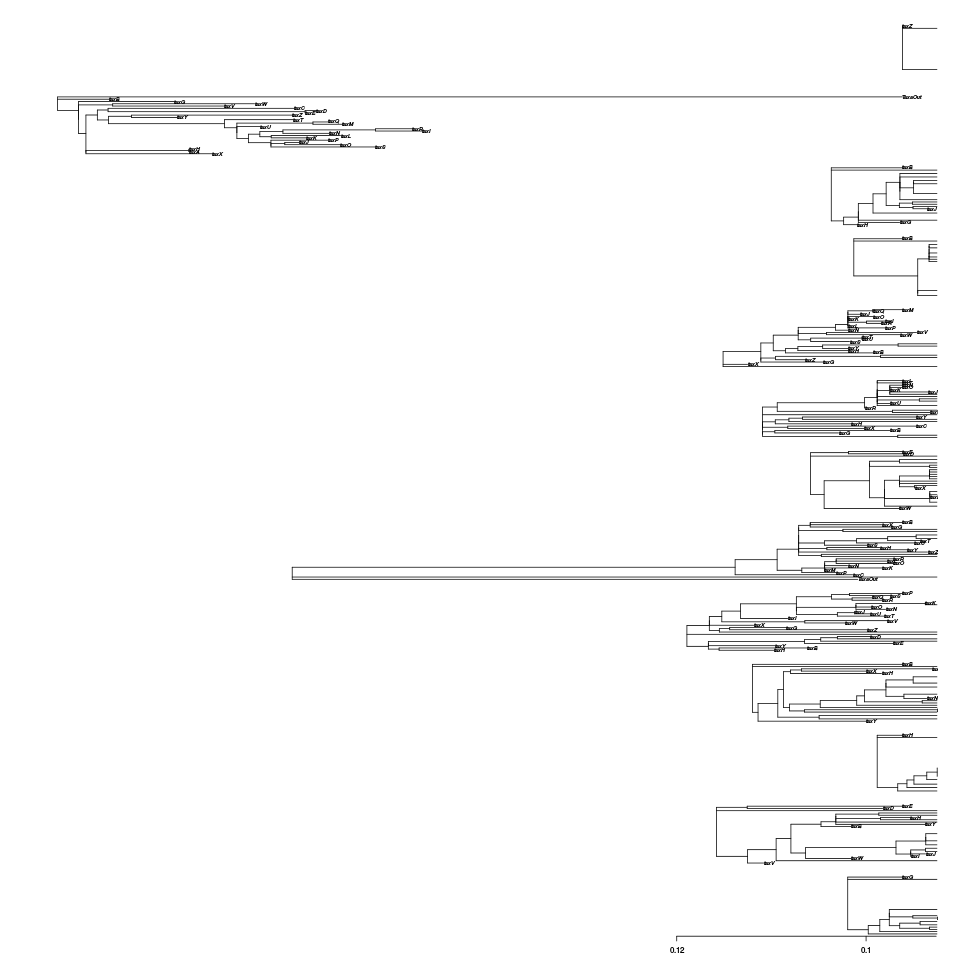
\includegraphics[height=5.5cm]{kronoviz.png}
  \columnbreak
  \begin{spluscode}
    kronoviz(x=oxalis.trees.rooted,
      layout=length(oxalis.trees.
      rooted), horiz=TRUE)
    # Close graphical device to
    # cancel division of plotting
    # device
    dev.off()
  \end{spluscode}
  \vfill
  The plot can be very long and it can be hard to see details. But one can get impression if all trees are more or less in same scale (have comparable length) or not.
\end{multicols}
\end{frame}

\subsection{MP}

\begin{frame}[fragile]{Maximum parsimony}
\begin{multicols}{2}
  \begin{spluscode}
    # Conversion to phyDat
    meles.phydat <-
      as.phyDat(meles.dna)
    # Prepare starting tree
    meles.tre.ini <- nj(dist.
      dna(x=meles.dna,model="raw"))
    # Parsimony: ?parsimony
    # Maximum parsimony score
    parsimony(tree=meles.tre.ini,
      data=meles.phydat)
    # Optimisation
    # Maximum parsimony tree
    meles.tre.pars <- optim.
      parsimony(tree=meles.tre.
      ini, data=meles.phydat)
    # Draw a tree
    plot.phylo(x=meles.tre.pars,
      type="clad", edge.width=2)
  \end{spluscode}
  \columnbreak
  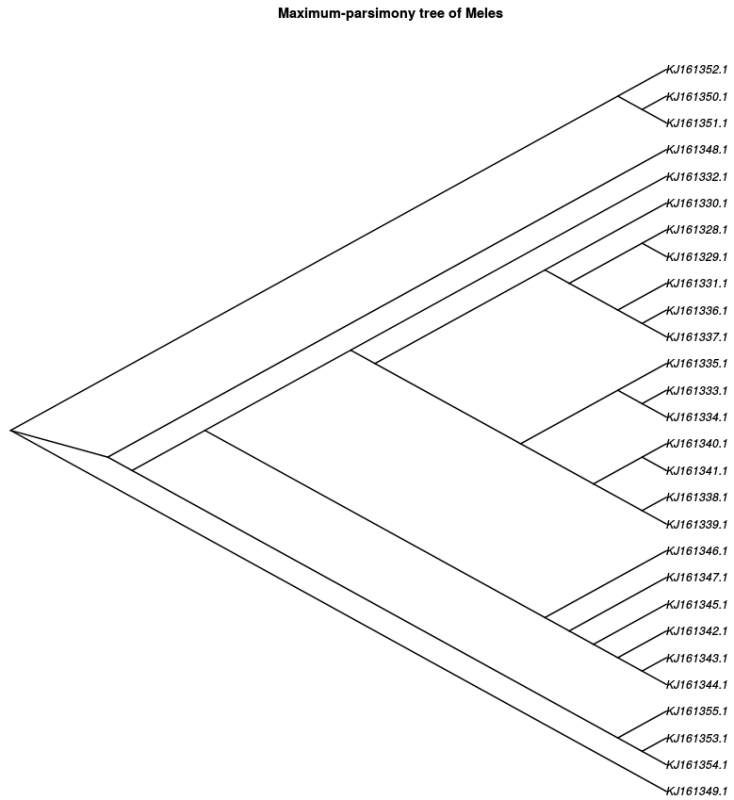
\includegraphics[height=6cm]{parsimony.png}
\end{multicols}
\end{frame}

\subsection{Notes about plotting the trees}

\begin{frame}[fragile]{Change orientation of plots}
\textbf{plot.phylo()} has plenty of possibilities to influence --- check \textbf{?plot.phylo} and \textbf{?par}
  \begin{spluscode}
    ?plot.phylo # check it for various possibilities what to influence
    par(mfrow=c(1, 2)) # Plot two plots in one row
    plot.phylo(x=hauss.nj, type="cladogram", use.edge.length=FALSE,
      direction="rightwards")
    plot.phylo(x=hauss.nj, type="cladogram", use.edge.length=FALSE,
      direction="leftwards")
    dev.off() # Close graphical device to cancel par() settings
  \end{spluscode}
\begin{center}
  \includegraphics[height=3cm]{lr.png}
\end{center}
\end{frame}

\begin{frame}[fragile]{Highlighted labels}
\begin{multicols}{2}
  \includegraphics[height=5cm]{highlight.png}
  \columnbreak
  \begin{spluscode}
    # Nice tiplabels and
    # higlighted tiplabel
    trape <- read.tree(text=
      "((Homo, Pan), Gorilla);")
    plot.phylo(x=trape,
      show.tip.label=FALSE)
    tiplabels(trape[["tip.label"]],
      bg=c("white", "black",
      "white"), col=c("black",
      "white", "black"))
    nodelabels(text=c("6.4 Ma",
      "5.4 Ma"), frame="circle",
      bg="white")
    add.scale.bar()
  \end{spluscode}
\end{multicols}
\end{frame}

\section{Evolution}

\subsection{PIC}

\begin{frame}[fragile]{Phylogenetic independent contrast}
\begin{itemize}
 \item When analysing comparative data takes phylogeny into account
 \item If we assume that a continuous trait evolves randomly in any direction (i.e., the Brownian motion model), then the ``contrast'' between two species is expected to have a normal distribution with mean zero, and variance proportional to the time since divergence
\end{itemize}
  \begin{spluscode}
    # Prepare the data # Body mass of primates
    primates.body <- c(4.09434, 3.61092, 2.37024, 2.02815, 1.46968)
    # Longevity of primates
    primates.longevity <- c(4.74493, 3.3322, 3.3673, 2.89037, 2.30259)
    # Add names to the values
    names(primates.body) <- names(primates.longevity) <- c("Homo", "Pongo",
      "Macaca", "Ateles", "Galago")
    # Create a tree in Newick format
    primates.tree <- read.tree(text="((((Homo:0.21, Pongo:0.21):0.28,
      Macaca:0.49):0.13, Ateles:0.62):0.38, Galago:1.00);")
    plot.phylo(primates.tree)
  \end{spluscode}
\end{frame}

\begin{frame}[fragile]{PIC and its plotting}
  \begin{spluscode}
    primates.pic.body <- pic(x=primates.body, phy=primates.tree,
      scaled=TRUE, var.contrasts=FALSE, rescaled.tree=FALSE)
    primates.pic.longevity <- pic(x=primates.longevity, phy=primates.tree,
      scaled=TRUE, var.contrasts=FALSE, rescaled.tree=FALSE)
    # Plot a tree with PIC values
    plot.phylo(x=primates.tree, lwd=2, cex=1.5, offset=0.2)
    nodelabels(round(primates.pic.body, digits=3), adj=c(0, -0.5),
      frame="none")
    nodelabels(round(primates.pic.longevity, digits=3), adj=c(0, 1),
      frame="none")
    add.scale.bar()
    # Plot PIC
    plot(x=primates.pic.body, y=primates.pic.longevity, pch=16, cex=1.5)
    abline(a=0, b=1, lty=2) # x=y line
    # correlation coefficient of both PICs
    cor(x=primates.pic.body, y=primates.pic.longevity, method="pearson")
    [1] -0.5179156
  \end{spluscode}
\end{frame}

\begin{frame}{Plot of PIC (on the tree)}
\includegraphics[width=\textwidth]{pic.png}
\end{frame}

\begin{frame}[fragile]{Test it}
  \begin{spluscode}
    lm(formula=primates.pic.longevity~primates.pic.body)
    Coefficients:
      (Intercept)  primates.pic.body
           1.6957            -0.3081
    # Because PICs have expected mean zero - such linear regressions
    # should be done through the origin (the intercept is set to zero)
    lm(formula=primates.pic.longevity~primates.pic.body-1)
    Coefficients:
    primates.pic.body
               0.4319
    # Permutation procedure to test PIC
    lmorigin(formula=primates.pic.longevity~primates.pic.body, nperm=1000)
    Regression through the origin
    Permutation method = raw data
    Coefficients and parametric test results
                       Coefficient Std_error t-value Pr(>|t|)
    primates.pic.body     0.43193   0.28649  1.5077   0.2288
    F-statistic: 2.273067 on 1 and 3 DF:
      permutational p-value: 0.2377622
  \end{spluscode}
\end{frame}

\subsection{Phylogenetic autocorrelation}

\begin{frame}[fragile]{Phylogenetic autocorrelation}
\begin{itemize}
 \item Autocorrelation coefficient to quantify whether the distribution of a trait among a set of species is affected or not by their phylogenetic relationships
 \item In the absence of phylogenetic autocorrelation, the mean expected value of I and its variance are known - it is thus possible to test the null hypothesis of the absence of dependence among observations
\end{itemize}
  \begin{spluscode}
    # Let's choose weights as wij = 1/dij, where the d’s is the distances
    # measured on the tree - cophenetic() calculates cophenetic distances
    # can be just cophenetic(primates.tree) or some other transformation
    primates.weights <- 1/cophenetic(primates.tree)
    primates.weights # See it
    class(primates.weights)
    diag(primates.weights) <- 0 # Set diagonal to 0
  \end{spluscode}
\end{frame}

\begin{frame}[fragile]{Testing of Moran's~\textit{I}}
  \begin{spluscode}
    # Calculate Moran's I
    # Slighly significant positive phylogenetic correlation among body mass
    Moran.I(x=primates.body, weight=primates.weights,
      alternative="greater")
    # Positive, but non-significant
    Moran.I(x=primates.longevity, weight=primates.weights,
      alternative="greater")
    # Test of Moran's with randomisation procedure
    # Body is significant - nonrandom, longevity not (random)
    gearymoran(bilis=primates.weights, X=data.frame(primates.body,
      primates.longevity), nrepet=1000)
    # Test of Abouheif designed to detect phylogenetic autocorrelation in a
    # quantitative trait - in fact Moran's I test using a particular
    # phylogenetic proximity between tips
    library(adephylo)
    abouheif.moran(x=cbind(primates.body, primates.longevity),
      W=primates.weights, method="oriAbouheif", a=1, nrepet=1000,
      alter="greater")
  \end{spluscode}
\end{frame}

\begin{frame}[fragile]{Correlogram to visualize results of phylogenetic autocorrelative analysis}
  \begin{spluscode}
    data(carnivora) # Loads training data set
    head(carnivora) # Look at the data
    # Calculate the correlogram
    carnivora.correlogram <- correlogram.formula
      (formula=SW~Order/SuperFamily/Family/Genus, data=carnivora)
    carnivora.correlogram # See results
    # Calculate the correlogram - test for both body masses
    carnivora.correlogram2 <- correlogram.formula
      (formula=SW+FW~Order/SuperFamily/Family/Genus, data=carnivora)
    carnivora.correlogram2 # See results
    plot.correlogram(x=carnivora.correlogram, legend=TRUE,
      test.level=0.05, col=c("white", "black")) # Plot it
    # Plot it - test for both body masses - two or one graph(s)
    plot.correlogramList(x=carnivora.correlogram2, lattice=TRUE,
      legend=TRUE, test.level=0.05)
    plot.correlogramList(x=carnivora.correlogram2, lattice=FALSE,
      legend=TRUE, test.level=0.05)
  \end{spluscode}
\end{frame}

\begin{frame}{Correlograms of SW and SW+FW (in one or two graphs) depending on taxonomical level with marked significance}
\includegraphics[width=\textwidth]{correlog.png}
\end{frame}

\subsection{pPCA}

\begin{frame}[fragile]{Phylogenetic principal component analysis}
  \begin{spluscode}
    # Library needed to create phylo4d object required by ppca
    library(phylobase)
    # Calculate pPCA
    primates.ppca <- ppca(x=phylo4d(x=primates.tree, cbind(
      primates.body, primates.longevity)), method="patristic",
      a=1, center=TRUE, scale=TRUE, scannf=TRUE, nfposi=1, nfnega=0)
    # Print results
    print.ppca(primates.ppca)
    # See summary information
    summary.ppca(primates.ppca)
    # See PCA scores for variables on phylogenetic tree
    scatter.ppca(primates.ppca)
    # See decomposition of pPCA eigenvalues
    screeplot.ppca(primates.ppca)
    # Plot pPCA results - global vs. local structure, decomposition
    # of pPCA eigenvalues, PCA plot of variables and PCA scores
    # for variables on phylogenetic tree
    plot.ppca(primates.ppca)
  \end{spluscode}
\end{frame}

\begin{frame}{Plot pPCA results - global vs. local structure, decomposition of pPCA eigenvalues, PCA plot of variables and PCA scores for variables on phylogenetic tree}
\includegraphics[width=\textwidth]{ppca.png}
\end{frame}

\subsection{Ancestral state reconstruction}

\begin{frame}[fragile]{Ancestral state reconstruction}
By default \textbf{ace} performs estimation for continuous characters assuming a Brownian motion model fit by maximum likelihood
  \begin{spluscode}
    # See ?ace for possible settings
    primates.body.ace <- ace(x=primates.body, phy=primates.tree,
      type="continuous", method="REML",
      corStruct=corBrownian(value=1, phy=primates.tree))
    # See result - reconstructions are in $ace
    # To be plotted on nodes - 1st column are node numbers
    primates.body.ace
    # Plot it
    plot(primates.tree, lwd=2, cex=2)
    tiplabels(round(primates.body, digits=3), adj=c(0, -1),
      frame="none", col="blue", cex=2)
    nodelabels(round(primates.body.ace$ace, digits=3),
    frame="circle", bg="red", cex=1.5)
  \end{spluscode}
Other implementations are available in packages geiger (functions fitContinuousMCMC and fitDiscrete), phangorn and more in ape (MPR)
\end{frame}

\begin{frame}{Ancestral state reconstructions of primates body weights}
\begin{center}
  \includegraphics[height=6.5cm]{ace.png}
\end{center}
\end{frame}

\section{The end}

\begin{frame}{Citations}
\begin{itemize}
  \item To correctly cite R launch \textbf{citation()} and see information there --- it is slightly different for every version of R
  \item Cite used packages --- launch \textbf{citation("PackageName")} --- if this information is missing, go to its manual page and/or homepage and find the information there
  \item Packages/functions commonly provide various methods to calculate desired task --- check function's help page (\textbf{\alert{?}FunctionName}) and find references there and cite them accordingly
\end{itemize}
\end{frame}

\subsection{Resources}

\begin{frame}[allowframebreaks]{Where to look for the help}
\begin{itemize}
 \item R phylogeny mailing list \href{https://stat.ethz.ch/mailman/listinfo/r-sig-phylo}{https://stat.ethz.ch/mailman/listinfo/r-sig-phylo}
 \item R genetics mailing list \href{https://stat.ethz.ch/mailman/listinfo/r-sig-genetics}{https://stat.ethz.ch/mailman/listinfo/r-sig-genetics}
 \item Bioconductor mailing list \href{https://stat.ethz.ch/mailman/listinfo/bioconductor}{https://stat.ethz.ch/mailman/listinfo/bioconductor} and Bioconductor help pages \href{http://master.bioconductor.org/help/}{http://master.bioconductor.org/help/}
 \item R phylo wiki \href{http://www.r-phylo.org/wiki/Main_Page}{http://www.r-phylo.org/wiki/Main\_Page}
 \item R phylogenetics at CRAN \href{http://cran.r-project.org/web/views/Phylogenetics.html}{http://cran.r-project.org/web/views/Phylogenetics.html}
 \item Little Book of R for Bioinformatics \href{http://a-little-book-of-r-for-bioinformatics.readthedocs.org/en/latest/}{http://a-little-book-of-r-for-bioinformatics.readthedocs.org/en/latest/}
 \item Adegenet web \href{http://adegenet.r-forge.r-project.org/}{http://adegenet.r-forge.r-project.org/} and help forum \href{https://lists.r-forge.r-project.org/cgi-bin/mailman/listinfo/adegenet-forum}{https://lists.r-forge.r-project.org/cgi-bin/mailman/listinfo/adegenet-forum}
 \item APE home page \href{http://ape-package.ird.fr/}{http://ape-package.ird.fr/}
 \item Phytools \href{http://phytools.org/}{http://phytools.org/} and its blog \href{http://blog.phytools.org/}{http://blog.phytools.org/}
 \item Poppr documentation and forum \href{http://grunwaldlab.cgrb.oregonstate.edu/poppr-r-package-population-genetics/manual-documentation-news-and-changes}{http://grunwaldlab.cgrb.oregonstate.edu/poppr-r-package-population-genetics/manual-documentation-news-and-changes}
 \item ade4 home page and documentation \href{http://pbil.univ-lyon1.fr/ade4/home.php?lang=eng}{http://pbil.univ-lyon1.fr/ade4/home.php?lang=eng}
 \item Phangorn resources \href{http://cran.r-project.org/web/packages/phangorn/index.html}{http://cran.r-project.org/web/packages/phangorn/index.html}
 \item Information and manual about pegas \href{http://ape-package.ird.fr/pegas.html}{http://ape-package.ird.fr/pegas.html}
 \item R help mailing list \href{https://stat.ethz.ch/mailman/listinfo/r-help}{https://stat.ethz.ch/mailman/listinfo/r-help} (web interface \href{http://r.789695.n4.nabble.com/}{http://r.789695.n4.nabble.com/})
 \item R announce mailing list \href{https://stat.ethz.ch/mailman/listinfo/r-announce}{https://stat.ethz.ch/mailman/listinfo/r-announce}
 \item R manuals \href{http://cran.r-project.org/manuals.html}{http://cran.r-project.org/manuals.html}
 \item Books about R \href{http://www.r-project.org/doc/bib/R-books.html}{http://www.r-project.org/doc/bib/R-books.html}
 \item R at StackOverflow StackExchange \href{https://stackoverflow.com/questions/tagged/r}{https://stackoverflow.com/questions/tagged/r}
 \item R at CrossValidated StackExchange \href{https://stats.stackexchange.com/questions/tagged/r}{https://stats.stackexchange.com/questions/tagged/r}
 \item The R journal \href{http://journal.r-project.org/}{http://journal.r-project.org/}
 \item R-bloggers --- aggregation of R blogs \href{http://www.r-bloggers.com/}{http://www.r-bloggers.com/}
 \item R on The Molecular Ecologist \href{http://www.molecularecologist.com/category/software/r/}{http://www.molecularecologist.com/category/software/r/}
 \item R tutorial \href{http://www.r-tutor.com/}{http://www.r-tutor.com/}
 \item Cookbook for R  \href{http://www.cookbook-r.com/}{http://www.cookbook-r.com/}
 \item spatial R \href{https://sites.google.com/site/spatialr/}{https://sites.google.com/site/spatialr/}
 \item Statistics with R \href{http://zoonek2.free.fr/UNIX/48_R/all.html}{http://zoonek2.free.fr/UNIX/48\_R/all.html}
 \item Springer R series \href{https://www.springer.com/series/6991?detailsPage=titles}{https://www.springer.com/series/6991?detailsPage=titles}
 \item Biostars --- general bioinformatics forum \href{https://www.biostars.org/}{https://www.biostars.org/}
 \item Biology --- general forum about biology at StackExchange \href{https://biology.stackexchange.com/}{https://biology.stackexchange.com/}
 \item Do not hesitate to ask on the forum or contact author of package with which you have problem, preferably through some public forum or mailing list, they usually respond quickly and helpfully\ldots
 \item \href{https://startpage.com/}{Uncle Google} is your friend (\textit{``how to XXX in R''})\ldots
 \item R packages commonly contain vignettes (tutorials) --- list them by \textbf{vignette()} and load selected by \textbf{vignette("VignetteName")}
 \item List available training datasets from various R packages by \textbf{data()} and load selected by \textbf{data(DatasetName)}
\end{itemize}
\end{frame}

\begin{frame}{Further reading}
\begin{thebibliography}{1}
  \bibitem[Crawley 2012]{Crawley2012}
    Michael J. Crawley
    \newblock The R Book, second edition
    \newblock Wiley, 2012
  \bibitem[Paradis 2012]{Paradis2012}
    Emmanuel Paradis
    \newblock Analysis of Phylogenetics and Evolution with R, second edition
    \newblock Springer, 2012
    \newblock \href{http://ape-package.ird.fr/APER.html}{http://ape-package.ird.fr/APER.html}
  \bibitem[Sinha 2014]{Sinha2014}
    Paurush Praveen Sinha
    \newblock Bioinformatics with R Cookbook
    \newblock Packt Publishing, 2014
\end{thebibliography}
\end{frame}

\subsection{The end}

\begin{frame}{The end}{Our course is over\ldots}
\begin{center}
  \ldots I hope it was helpful for You\ldots\\
  \vfill
  \ldots any feedback is welcomed\ldots
  \vfill
  \ldots happy \textbf{\textit{R}} hacking\ldots
  \vfill
\end{center}
\begin{flushright}
  \begin{tiny}
   \href{http://www.xelatex.org/}{Typesetting} using \XeLaTeX~on \href{http://www.opensuse.org/}{openSUSE} \href{https://en.wikipedia.org/wiki/GNU}{GNU}/\href{https://en.wikipedia.org/wiki/Linux}{Linux}
  \end{tiny}
\end{flushright}
\end{frame}

\end{document}
